\documentclass[runningheads,a4paper]{llncs}

\def\incolour{T}

\usepackage[paperwidth=15cm, paperheight=22cm, textwidth=12.2cm, textheight=19.3cm, inner=1.4cm, outer=1.4cm]{geometry}

\ifdefined\incolour
\def\myblue{blue}
\def\myred{red}
\def\mypurple{MediumPurple}
\def\mygreen{SeaGreen}
\def\mybrown{Chocolate}
\else
\def\myblue{black}
\def\myred{black}
\def\mypurple{black}
\def\mygreen{black}
\def\mybrown{black}
\fi

\renewcommand{\rmdefault}{ptm}

\newcommand{\ribboncolor}{black!15}
\newcommand{\varcolor}{black!21}
\newcommand{\ribbonouterborderthickness}{0.6}
\newcommand{\casesborderthickness}{0.6}
\newcommand{\casesbordercolor}{black}
\newcommand{\commandcolor}{black}
\newcommand{\juscolor}{black!55}
\newcommand{\commandtextcolor}{white}
\newcommand{\shadowcolor}{black!40}

\usepackage[caption=false,font=footnotesize]{subfig}
\usepackage{wrapfig}
\usepackage{multicol}
\usepackage{datetime}
\usepackage{framed}

\usepackage{JohnMath}
\renewcommand{\true}{\ensuremath{\mathit{true}}}
\renewcommand{\false}{\ensuremath{\mathit{false}}}
\renewcommand{\emp}{\ensuremath{\mathit{emp}}}
\renewcommand{\dom}{\mathop{\mathit{dom}}}
\usepackage{calc}

\usepackage[svgnames]{xcolor}
\usepackage{tikz}
\usetikzlibrary{positioning}
\usetikzlibrary{patterns}

\usepackage{rotating}
\newcommand{\mrot}[1]{\raisebox{1.7ex}{\turnbox{270}{\ensuremath{\begin{array}{@{}l@{}}#1\end{array}}}}}

\newcommand{\semi}[1][]{\mathbin{\text{\bf ;}}}
\newcommand{\stacker}[3][0mm]{{\begin{array}{@{}c@{}}#2 \\[#1] #3\end{array}}}
\newcommand{\tstacker}[2]{\genfrac{}{}{0pt}{1}{#1}{#2}}

% CODE LISTINGS
\usepackage{listings}
\lstset{
  language=,
  columns=[l]fullflexible,
  mathescape=true,
  basicstyle=\ttfamily,%\color{Purple},
  showstringspaces=false,
  commentstyle=\color{DarkGreen}, 
  numbers=none, 
  escapechar=£,
  escapebegin=\rmfamily\color{Black}
}
%\newcommand{\code}[1]{\texttt{#1}}

% SPECIFICATIONS
\newcommand{\ml}[2][t]{\mbox{\mdseries\begin{tabular}[#1]{@{}L@{}}#2\end{tabular}}}
\newcommand{\ass}[1]{\ensuremath{{\color{black}\left\{\ml[c]{#1}\right\}}}}
\newcommand{\seqspec}[3]{\ass{#1}\,{\mbox{\code{#2}}}\,\ass{#3}}
\newcommand{\Seqspec}[3]{\multicolumn{2}{l}{$\ass{#1}$ {#2} $\ass{#3}$}}
\newcommand{\comm}[1]{\vspace{-2pt}%
    \begin{list}{/$*$}{%
        \topsep=5pt%
        \leftmargin=3cm%
      }\item #1 \hfill$*$/\end{list}%
}

\newcommand{\floorpow}[1]{\llfloor{#1}\rrfloor}
\newcommand{\fracpow}[1]{\{\hspace{-3pt}\{{#1}\}\hspace{-3pt}\}}
\newcommand{\defined}{\mathop{\text{def}}}

\newcommand{\ribbon}[1]{
\tikz[x=1mm, y=1mm, baseline=0]{
\node[anchor=base, style={rectangle, fill=\ribboncolor}] (step) at (0,0) {\ensuremath{#1}};
}
}

\newcommand{\closedribbon}[1]{\ribbon{#1}}

\newcommand{\existsbox}[2]{\hspace{2mm}\rule[-0.5mm]{0.2mm}{1mm}\raisebox{1mm}{\hspace{-2mm} {\scriptsize $∃ #1$}}{#2}\,\rule[-0.5mm]{0.2mm}{3mm}}

\newcommand{\closedexistsbox}[2]{\,\ensuremath{\tikz[x=1mm,y=1mm,baseline=0mm]{
\node[anchor=base west, style={rectangle, draw=black}] at (0,0) {\,\ensuremath{#2}\!};
\node[style={rectangle, fill=white, inner sep=0.2mm}] at (0,1.6) {\scriptsize $∃ #1$};
}}\,}

\newcommand{\ditto}{\ensuremath{\prime\prime}}

\newcommand{\assn}{\mathop{\mathit{asn}}}
\newcommand{\WR}{\mathop{\mathit{wr}}}
\newcommand{\RD}{\mathop{\mathit{rd}}}
\newcommand{\ileave}[1][]{\mathop{\mathit{zip}_{#1}}}

\newcommand{\nakedbasicstep}[2][8]{
\def\greybarrad{1.7}
\def\greybarwidth{#1}
\tikz[x=1mm, y=1mm, baseline=0]{
\node[anchor=base, style={rectangle, minimum width=\greybarwidth mm, minimum height = 2*\greybarrad mm, fill=\commandcolor}] (step) at (0,0) {\color{\commandtextcolor}{\ensuremath{#2}}};
}
}

\newcommand{\basicstep}[4][8]{
\def\greybarrad{1.7}
\def\greybarwidth{#1}
\tikz[x=1mm, y=1mm, baseline=0]{
\node[anchor=base, style={rectangle, minimum width=\greybarwidth mm, minimum height = 2*\greybarrad mm, fill=\commandcolor}] (step) at (0,0) {\color{\commandtextcolor}{\ensuremath{#3}}};
\node[above=-0.5mm of step.north]{\ensuremath{#2}};
\node[below=-0.5mm of step.south]{\ensuremath{#4}};
}
}

\newcommand{\nakedloopdia}[2][9]{
\def\greybarrad{1.7}
\def\greybarwidth{#1}
\tikz[x=1mm, y=-1mm, baseline=-2.4mm]{
\filldraw [fill=\commandcolor, draw=\commandcolor, ultra thick, rounded corners=\greybarrad mm] (-\greybarwidth/2,-\greybarrad-0.8) rectangle (\greybarwidth/2,\greybarrad-0.8);
\filldraw [fill=\commandcolor, draw=\commandcolor, ultra thick] (-\greybarwidth/2, -0.8) rectangle (\greybarwidth/2,\greybarrad-0.8);
\draw (-\greybarwidth/2,0) node[anchor=base west] {\color{\commandtextcolor}{{\tt loop}}};
\draw (0,4.4) node[anchor=base] {\ensuremath{#2}};
\draw [\commandcolor, ultra thick, rounded corners=\greybarrad mm] (-\greybarwidth/2,-\greybarrad-0.8) rectangle (\greybarwidth/2,\greybarrad-0.8+4.6);
%\filldraw [fill=white, draw=lightgray, ultra thick] (-\greybarwidth/2, -0.8+8.4-\greybarrad) rectangle (\greybarwidth/2,-0.8+8.4);
}
}

\newcommand{\loopdia}[4][9]{
\def\greybarrad{1.7}
\def\greybarwidth{#1}
\tikz[x=1mm, y=-1mm, baseline=-2.4mm]{
\filldraw [fill=\commandcolor, draw=\commandcolor, ultra thick, rounded corners=\greybarrad mm] (-\greybarwidth/2,-\greybarrad-0.8) rectangle (\greybarwidth/2,\greybarrad-0.8);
\filldraw [fill=\commandcolor, draw=\commandcolor, ultra thick] (-\greybarwidth/2, -0.8) rectangle (\greybarwidth/2,\greybarrad-0.8);
\draw (0,-3.6) node[anchor=base] {\ensuremath{#2}};
\draw (-\greybarwidth/2,0) node[anchor=base west] {\color{\commandtextcolor}{{\tt loop}}};
\draw (0,4.4) node[anchor=base] {\ensuremath{#3}};
\draw [\commandcolor, ultra thick, rounded corners=\greybarrad mm] (-\greybarwidth/2,-\greybarrad-0.8) rectangle (\greybarwidth/2,\greybarrad-0.8+4.6);
\draw (0,8.4) node[anchor=base] {\ensuremath{#4}};
}
}

\newcommand{\nakedchoicedia}[3][9]{
\def\greybarrad{1.7}
\def\greybarwidth{#1}
\tikz[x=1mm, y=-1mm, baseline=-8.4mm]{
\draw [\commandcolor,ultra thick, rounded corners=\greybarrad mm] (-\greybarwidth/2,-\greybarrad+2.8) rectangle (\greybarwidth/2,-0.8+14.8);
\draw (0,4.4) node[anchor=base] {\ensuremath{#2}};
\filldraw [fill=\commandcolor, draw=\commandcolor, ultra thick] (-\greybarwidth/2,-\greybarrad-0.8+8.4) rectangle (\greybarwidth/2,\greybarrad-0.8+8.4);
\draw (0,8.4) node[anchor=base] {\color{\commandtextcolor}{{\tt or}}};
\draw (0,12.6) node[anchor=base] {\ensuremath{#3}};
}
}

\newcommand{\choicedia}[5][9]{
\def\greybarrad{1.7}
\def\greybarwidth{#1}
\tikz[x=1mm, y=-1mm, baseline=-8.4mm]{
\draw (0,0) node[anchor=base] {\ensuremath{#2}};
\draw [\commandcolor,ultra thick, rounded corners=\greybarrad mm] (-\greybarwidth/2,-\greybarrad+2.8) rectangle (\greybarwidth/2,-0.8+14.8);
\draw (0,4.4) node[anchor=base] {\ensuremath{#3}};
\filldraw [fill=\commandcolor, draw=\commandcolor, ultra thick] (-\greybarwidth/2,-\greybarrad-0.8+8.4) rectangle (\greybarwidth/2,\greybarrad-0.8+8.4);
\draw (0,8.4) node[anchor=base] {\color{\commandtextcolor}{{\tt or}}};
\draw (0,12.6) node[anchor=base] {\ensuremath{#4}};
\draw (0,17) node[anchor=base] {\ensuremath{#5}};
}
}

\newcommand{\coms}{\mathop{\mathit{coms}}}
\newcommand{\lin}{\mathop{\mathit{lin}}}
\newcommand{\links}{\mathop{\mathit{links}}}
\newcommand{\orders}{\mathop{\mathit{orders}}}
\newcommand{\Dsem}[1]{\sem{#1}_{\rm dia}}
\newcommand{\Isem}[1]{\sem{#1}_{\rm int}}
\newcommand{\arrowuplus}{\mathbin{\stackrel{→}{\uplus}}}
\newcommand{\arrowparallel}{\stackrel{→}{\parallel}}
\newcommand{\TOP}{\mathop{\mathit{top}}}
\newcommand{\BOT}{\mathop{\mathit{bot}}}
\newcommand{\terminals}{\mathop{\mathit{terminals}}}
\newcommand{\initials}{\mathop{\mathit{initials}}}
\newcommand{\COM}{\mathop{\mathit{com}}}
\newcommand{\process}{\mathop{\mathit{exec}}}
\newcommand{\chains}{\mathop{\mathit{chains}}}
\newcommand{\acyclic}{\mathop{\mathit{acyclic}}}
\newcommand{\linear}{\mathop{\mathit{linear}}}

%\newcommand{\isabelle}{\raisebox{0.3mm}{\renewcommand{\arraystretch}{0.53}\begin{tabular}{@{}|@{}c@{}|@{}}\hline\scalebox{0.52} {\:Isabelle\:}\\\hline\end{tabular}}}

%\newcommand{\isabelle}{\raisebox{0.2mm}{\renewcommand{\arraystretch}{0.4}\begin{tabular}{@{}|@{}c@{}|@{}}\hline \\[-1mm] {\:{\small Isabelle}\:}\\\hline\end{tabular}}}

\newcommand{\isabelle}{

\begin{tikzpicture}[x=0.8mm, y=0.8mm, baseline=-0.3mm, line join=round]
\begin{scope}[yslant=-0.5]
  \draw (0,0) rectangle (1,1);
  \draw (2,1) rectangle (3,2);
  \draw (1,2) rectangle (2,3);
\end{scope}
\begin{scope}[yslant=0.5]
  \filldraw[black] (1,-1) rectangle (2,0);
  \filldraw[black] (3,-2) rectangle (4,-1);
  \filldraw[black] (2,0) rectangle (3,1);
\end{scope}
\begin{scope}[yslant=0.5,xslant=-1]
  \draw (1,0) rectangle (2,1);
  \draw (2,-1) rectangle (3,0);
  \draw (3,1) rectangle (4,2);
\end{scope}
\end{tikzpicture}
}

\hyphenation{as-sump-tion in-ter-me-di-ate as-ser-tion white-space}

\title{Ribbon Proofs for Separation Logic }

\author{John Wickerson\inst{1} \and Mike Dodds\inst{2} \and Matthew Parkinson\inst{3}}
\institute{Technische Universität Berlin, Germany \and University of York, United Kingdom \and Microsoft Research Cambridge, United Kingdom}

\begin{document}

\maketitle

\setcounter{footnote}{0}

\begin{abstract}
We present \emph{ribbon proofs}, a diagrammatic system for proving program correctness based on separation logic. Ribbon proofs emphasise the structure of a proof, so are intelligible and pedagogical. Because they contain less redundancy than proof outlines, and allow each proof step to be checked locally, they may be more scalable. Where proof outlines are cumbersome to modify, ribbon proofs can be visually manoeuvred to yield proofs of variant programs. This paper introduces the ribbon proof system, proves its soundness and completeness, and outlines a prototype tool for validating the diagrams in \emph{Isabelle}.
\end{abstract}

\section{Introduction}

A program proof should not merely certify \emph{that} a program is correct; it should explain \emph{why} it is correct. A proof should be more than `true': it should be informative, and it should be intelligible. This paper does not contribute new methods for proving more properties of more programs, but rather, a new way to present such proofs. Building on work by Bean~\cite{bean06}, we present a system that produces program proofs in separation logic that are readable, scalable, and easily modified.

A program proof in Hoare logic~\cite{hoare69} is usually presented as a \emph{proof outline}, in which the program's instructions are interspersed with `enough' assertions to allow the reader to reconstruct the derivation tree. Since emerging circa 1971, the proof outline has become the de facto standard in the literature on both Hoare logic (e.g.~\cite{ashcroft76,hoare71,owicki+76,schneider97}) and its recent descendant, separation logic (e.g.~\cite{bornat+05,dinsdale-young+10-b,dodds+09,feng09,feng+07-a,gotsman+07,hur+11,ishtiaq+01,jacobs+11,reynolds02,vafeiadis+07%,berdine+05,bornat+04,gardner+09,botincan+11,kapoor+11,
}). Its great triumph is what might be called \emph{instruction locality}: that one can verify each instruction in isolation (by confirming that the assertions immediately above and below it form a valid Hoare triple) and immediately deduce that the entire proof is correct. 

\begin{figure}[t]%
\centering
\subfloat[A proof outline]{%
\label{fig:proofoutline}%
\renewcommand{\arraystretch}{1.15}
\begin{tabular}{@{}l@{~~}l@{}}
{\scriptsize 1}&{\renewcommand{\arraystretch}{1}\ass{\code{x}↦0 * \code{y}↦0 * \code{z}↦0}} \\
{\scriptsize 2}&~~\code{[x]:=1;} \\
{\scriptsize 3}&{\renewcommand{\arraystretch}{1}\ass{\code{x}↦1 * \code{y}↦0 * \code{z}↦0}} \\
{\scriptsize 4}&~~\code{[y]:=1;} \\
{\scriptsize 5}&{\renewcommand{\arraystretch}{1}\ass{\code{x}↦1 * \code{y}↦1 * \code{z}↦0}} \\
{\scriptsize 6}&~~\code{[z]:=1;} \\
{\scriptsize 7}&{\renewcommand{\arraystretch}{1}\ass{\code{x}↦1 * \code{y}↦1 * \code{z}↦1}}
\end{tabular}%
}%
\hspace{2cm} 
\subfloat[A ribbon proof]{%
\begin{minipage}{1.6in}
\label{fig:assignment_ribbonproof}%
\begin{center}
\noindent%Starting.
\pgfdeclarelayer{frontmost}
\pgfdeclarelayer{colnameslayer}
\pgfsetlayers{main,frontmost,colnameslayer}
\begin{tikzpicture}[x=1mm,y=1mm,scale=1.]
% State has been set.
\draw [line width = 0.5mm, white] (1.,0.) -- (1.,-5.);
\draw [line width = 0.5mm, white] (13.,0.) -- (13.,-5.);
\fill [black!15] (1.,0.) -- (1.,-5.) -- (13.,-5.) -- (13.,0.) -- cycle;
\begin{pgfonlayer}{frontmost}
\draw [black] (7.,-3.) node{\smash{$\ml[t]{\code{x}↦0}$}};
\end{pgfonlayer}
\draw [line width = 0.5mm, white] (15.,0.) -- (15.,-5.);
\draw [line width = 0.5mm, white] (27.,0.) -- (27.,-5.);
\fill [black!15] (15.,0.) -- (15.,-5.) -- (27.,-5.) -- (27.,0.) -- cycle;
\begin{pgfonlayer}{frontmost}
\draw [black] (21.,-3.) node{\smash{$\ml[t]{\code{y}↦0}$}};
\end{pgfonlayer}
\draw [line width = 0.5mm, white] (29.,0.) -- (29.,-5.);
\draw [line width = 0.5mm, white] (41.,0.) -- (41.,-5.);
\fill [black!15] (29.,0.) -- (29.,-5.) -- (41.,-5.) -- (41.,0.) -- cycle;
\begin{pgfonlayer}{frontmost}
\draw [black] (35.,-3.) node{\smash{$\ml[t]{\code{z}↦0}$}};
\end{pgfonlayer}
\begin{pgfonlayer}{frontmost}
\fill[fill=black] (1.,-10.) rectangle (13.,-5.);
\draw [white] (1.,-7.5) node[anchor=west]{\code{\begin{tabular}{@{\hspace{-0.8mm}}l@{\hspace{-0.8mm}}}[x]:=1\end{tabular}}};
\end{pgfonlayer}
\draw [line width = 0.5mm, white] (15.,-5.) -- (15.,-10.);
\draw [line width = 0.5mm, white] (27.,-5.) -- (27.,-10.);
\fill [black!15] (15.,-5.) -- (15.,-10.) -- (27.,-10.) -- (27.,-5.) -- cycle;
\draw [line width = 0.5mm, white] (29.,-5.) -- (29.,-10.);
\draw [line width = 0.5mm, white] (41.,-5.) -- (41.,-10.);
\fill [black!15] (29.,-5.) -- (29.,-10.) -- (41.,-10.) -- (41.,-5.) -- cycle;
\draw [line width = 0.5mm, white] (29.,-10.) -- (29.,-13.);
\draw [line width = 0.5mm, white] (41.,-10.) -- (41.,-13.);
\fill [black!15] (29.,-10.) -- (29.,-13.) -- (41.,-13.) -- (41.,-10.) -- cycle;
\draw [line width = 0.5mm, white] (1.,-10.) -- (1.,-13.);
\draw [line width = 0.5mm, white] (13.,-10.) -- (13.,-13.);
\fill [black!15] (1.,-10.) -- (1.,-13.) -- (13.,-13.) -- (13.,-10.) -- cycle;
\begin{pgfonlayer}{frontmost}
\draw [black] (7.,-13.) node{\smash{$\ml[t]{\code{x}↦1}$}};
\end{pgfonlayer}
\draw [line width = 0.5mm, white] (15.,-10.) -- (15.,-13.);
\draw [line width = 0.5mm, white] (27.,-10.) -- (27.,-13.);
\fill [black!15] (15.,-10.) -- (15.,-13.) -- (27.,-13.) -- (27.,-10.) -- cycle;
\begin{pgfonlayer}{frontmost}
\fill[fill=black] (15.,-18.) rectangle (27.,-13.);
\draw [white] (15.,-15.5) node[anchor=west]{\code{\begin{tabular}{@{\hspace{-0.8mm}}l@{\hspace{-0.8mm}}}[y]:=1\end{tabular}}};
\end{pgfonlayer}
\draw [line width = 0.5mm, white] (1.,-13.) -- (1.,-18.);
\draw [line width = 0.5mm, white] (13.,-13.) -- (13.,-18.);
\fill [black!15] (1.,-13.) -- (1.,-18.) -- (13.,-18.) -- (13.,-13.) -- cycle;
\draw [line width = 0.5mm, white] (29.,-13.) -- (29.,-18.);
\draw [line width = 0.5mm, white] (41.,-13.) -- (41.,-18.);
\fill [black!15] (29.,-13.) -- (29.,-18.) -- (41.,-18.) -- (41.,-13.) -- cycle;
\draw [line width = 0.5mm, white] (1.,-18.) -- (1.,-21.);
\draw [line width = 0.5mm, white] (13.,-18.) -- (13.,-21.);
\fill [black!15] (1.,-18.) -- (1.,-21.) -- (13.,-21.) -- (13.,-18.) -- cycle;
\draw [line width = 0.5mm, white] (15.,-18.) -- (15.,-21.);
\draw [line width = 0.5mm, white] (27.,-18.) -- (27.,-21.);
\fill [black!15] (15.,-18.) -- (15.,-21.) -- (27.,-21.) -- (27.,-18.) -- cycle;
\begin{pgfonlayer}{frontmost}
\draw [black] (21.,-21.) node{\smash{$\ml[t]{\code{y}↦1}$}};
\end{pgfonlayer}
\draw [line width = 0.5mm, white] (29.,-18.) -- (29.,-21.);
\draw [line width = 0.5mm, white] (41.,-18.) -- (41.,-21.);
\fill [black!15] (29.,-18.) -- (29.,-21.) -- (41.,-21.) -- (41.,-18.) -- cycle;
\begin{pgfonlayer}{frontmost}
\fill[fill=black] (29.,-26.) rectangle (41.,-21.);
\draw [white] (29.,-23.5) node[anchor=west]{\code{\begin{tabular}{@{\hspace{-0.8mm}}l@{\hspace{-0.8mm}}}[z]:=1\end{tabular}}};
\end{pgfonlayer}
\draw [line width = 0.5mm, white] (1.,-21.) -- (1.,-26.);
\draw [line width = 0.5mm, white] (13.,-21.) -- (13.,-26.);
\fill [black!15] (1.,-21.) -- (1.,-26.) -- (13.,-26.) -- (13.,-21.) -- cycle;
\draw [line width = 0.5mm, white] (15.,-21.) -- (15.,-26.);
\draw [line width = 0.5mm, white] (27.,-21.) -- (27.,-26.);
\fill [black!15] (15.,-21.) -- (15.,-26.) -- (27.,-26.) -- (27.,-21.) -- cycle;
\draw [line width = 0.5mm, white] (1.,-26.) -- (1.,-30.);
\draw [line width = 0.5mm, white] (13.,-26.) -- (13.,-30.);
\fill [black!15] (1.,-26.) -- (1.,-30.) -- (13.,-30.) -- (13.,-26.) -- cycle;
\draw [line width = 0.5mm, white] (15.,-26.) -- (15.,-30.);
\draw [line width = 0.5mm, white] (27.,-26.) -- (27.,-30.);
\fill [black!15] (15.,-26.) -- (15.,-30.) -- (27.,-30.) -- (27.,-26.) -- cycle;
\draw [line width = 0.5mm, white] (29.,-26.) -- (29.,-30.);
\draw [line width = 0.5mm, white] (41.,-26.) -- (41.,-30.);
\fill [black!15] (29.,-26.) -- (29.,-30.) -- (41.,-30.) -- (41.,-26.) -- cycle;
\begin{pgfonlayer}{frontmost}
\draw [black] (35.,-29.) node{\smash{$\ml[t]{\code{z}↦1}$}};
\end{pgfonlayer}
\end{tikzpicture}
%Finished.

\end{center}
\end{minipage}
}%
\caption{A simple example}
\label{fig:assignment}
\end{figure}

Yet proof outlines also suffer several shortcomings, some of which are manifested in Fig.~\ref{fig:proofoutline}. This proof outline concerns a program that writes to three memory cells, which separation logic's \mbox{$*$-operator} deems distinct. First, it is highly repetitive: `$\code{x}↦1$' appears three times. Second, it is difficult to interpret the effect of each instruction, there being no distinction between those parts of an assertion that are actively involved and those that are merely in what separation logic calls the \emph{frame}. For instance, line~4 affects only the second conjunct of its preceding assertion, but it is difficult to deduce the assignment's effect because two unchanged conjuncts are also present. Of course, these are only minor problems in our toy example, but they quickly become devastating when scaled to serious programs.

The crux of the problem is what might be called \emph{resource locality}. Separation logic~\cite{ishtiaq+01,reynolds02} specialises in this second dimension of locality. One can use separation logic's \emph{small axioms} to reason about each instruction as if it were executing in a state containing only the resources (i.e.\ memory cells) that it needs, and immediately deduce its effect on the entire state using the \emph{frame rule}. The proof outline below depicts this mechanism for line 4 of Fig.~\ref{fig:proofoutline}. 
\[
\small
\begin{array}{@{}l}\text{frame}\\\code{x}↦1 * \code{z}↦0\end{array} ~ \textrm{-}\hspace{-5.5pt}\left[\begin{array}{l}
\ass{\code{x}↦1 * \code{y}↦0 * \code{z}↦0} \\[1mm]
\left.\begin{array}{@{}l}
~~\ass{\code{y}↦0}\\[1mm]
~~~~\code{[y]:=1;}\\[1mm]
~~\ass{\code{y}↦1}
\end{array}\qquad\qquad\qquad\right]\hspace{-5.5pt}\textrm{-} \begin{array}{l@{}}\text{small axiom}\\\text{for heap update}\end{array} \\
\ass{\code{x}↦1 * \code{y}↦1 * \code{z}↦0}
\end{array}\right.
\]
Showing such detail throughout a proof outline would clarify the effect of each instruction, but escalate the repetition. Cleverer use of the frame rule can help, but only a little -- see Sect.~\ref{sect:future}. Essentially, we need a new proof representation to harness the new technology separation logic provides, and we propose the {\bf ribbon proof}.

Figure~\ref{fig:assignment_ribbonproof} gives an example. The repetition has disappeared, and each instruction's effect is now clear: it affects exactly those assertions directly above and below it, while framed assertions (which must not mention variables written by the instruction) pass unobtrusively to the left or right. Technically, we are still invoking the frame rule at each instruction, but crucially in a ribbon proof, such invocations are implicit and do not complicate the diagram.

A bonus of this particular ribbon proof is that it emphasises that the three assignments update different memory cells. They are thus independent, and amenable to reordering or parallelisation. One can imagine obtaining a proof of the transformed program by simply sliding the left-hand column downward and the right-hand column upward. The corresponding proof outline neither suggests nor supports such manoeuvres. 

Where a proof outline essentially flattens a proof to a list of assertions and instructions, our system produces geometric objects that can be navigated and modified by leveraging human visual intuition, and whose basic steps correspond exactly to separation logic's small axioms. A ribbon proof de-emphasises the program's shallow syntax, such as the order of independent instructions, and illuminates instead the deeper structure, such as the flow of resources through the code. Proof outlines focus on Hoare triples $\{p\}\,c\,\{q\}$, and often neglect the details of entailments between assertions, $p⇒q$, even though such entailments often encode important insights about the program being verified. Ribbon proofs treat both types of judgement equally, within the same system.

There are many recent extensions of separation logic (e.g.~\cite{dinsdale-young+13,dinsdale-young+10-b,dodds+09,feng09,feng+07-a,gotsman+07,hur+11,jacobs+11,ohearn07,vafeiadis+07%,kapoor+11
}) to which our ribbon proof technology can usefully be applied; indeed, ribbons have already aided the development of a separation logic for relaxed memory~\cite{bornat+12}. All of these program logics are based on increasingly complex reasoning principles, of which clear explanations are increasingly vital. We propose ribbon proofs as the ideal device for providing them.

\subsubsection{Comparison with Bean's system} Bean~\cite{bean06} introduced ribbon proofs as an extension of Fitch's \emph{box proofs}~\cite{fitch52} to handle the propositional fragment of bunched implications logic (BI)~\cite{ohearn+99}. BI being the basis of separation logic's assertion language~\cite{ishtiaq+01}, his system can be used to prove entailments between propositional separation logic assertions. Our system expands Bean's into a full-blown program logic by adding support for commands and existentially-quantified variables. It is further distinguished by its treatment of ribbon proofs as graphs, which gives our diagrams an appealing degree of flexibility.

\subsubsection*{Contributions and paper outline} We describe a diagrammatic proof system that enables a natural presentation of separation logic proofs. We prove it sound and complete with respect to separation logic (Sect.~\ref{sect:formalisation}). We also give an alternative, graphical formalisation (Sect.~\ref{sect:v_a_r}), which is sound in the absence of the frame rule's side-condition.

We describe a prototype tool (Sect.~\ref{sect:tool}) for mechanically checking ribbon proofs with the \emph{Isabelle} proof assistant. Given a small proof script for each basic step, our tool assembles a script that verifies the entire diagram. Such tediums as the associativity and commutativity of~$*$ are handled in the graphical structure, leaving the user to focus on the interesting parts of the proof. 

We discuss (Sect.~\ref{sect:future}) extensions to handle concurrent separation logic, possible applications to parallelisation, and connections to proof nets, bigraphs and string diagrams.

We begin by introducing our ribbon proof system with the aid of an example. Further examples can be found in Wickerson's PhD dissertation~\cite{wickerson13}. Of those, our ribbon proof of the Version 7 Unix memory manager demonstrates that our system can present readable proofs of more complex programs than those considered in this paper.

\section{An example}\label{sect:informal_development}

\newcommand{\lseg}[2]{\mathit{ls}\,{#1}\,{#2}}
\newcommand{\List}[2]{\mathit{list}\,{#1}\,{#2}}

\newcommand{\rev}[1]{#1^\dagger}

\begin{figure}[t]
\centering
\def\ang{20}
\tikzstyle{ribbon}=[fill = black!15]
\tikzstyle{bendribbon}=[shade,
                        top color = white,
                        bottom color = black!30,
                        shading angle = \ang]
\tikzstyle{backbend}=[shading angle = 180+\ang]
\def\yb{5.5}
\def\yc{7}
\def\x{1}
\def\w{1.5}
{\small (a)}~~$\begin{array}{@{}l@{}}
\vspace{-3mm}
%\makeribbonproof{whilestatement.tex}{1}
\noindent%Starting.
\pgfdeclarelayer{frontmost}
\pgfdeclarelayer{colnameslayer}
\pgfsetlayers{main,frontmost,colnameslayer}
\begin{tikzpicture}[x=1mm,y=1mm,scale=1.]
% State has been set.
\begin{pgfonlayer}{frontmost}
\draw [black] (13.5,-3.) node{\smash{$\ml[t]{A}$}};
\end{pgfonlayer}
\draw [line width = 0.6mm, black] (1.65,-10.) -- (1.65,-9.);
\draw [line width = 0.6mm, black] (25.35,-10.) -- (25.35,-9.);
\fill[fill=black, rounded corners=2.mm] (1.3,-9.) rectangle (25.7,-4.);
\fill[fill=black] (1.3,-9.) rectangle (25.7,-6.5);
\draw [white] (1.3,-6.5) node[anchor=west]{\code{while (...) \{}};
\draw [line width = 0.6mm, black] (1.65,-13.) -- (1.65,-9.);
\draw [line width = 0.6mm, black] (25.35,-13.) -- (25.35,-9.);
\begin{pgfonlayer}{frontmost}
\draw [black] (13.5,-12.) node{\smash{$\ml[t]{B}$}};
\end{pgfonlayer}
\draw [line width = 0.6mm, black] (1.65,-13.) -- (1.65,-12.);
\draw [line width = 0.6mm, black] (25.35,-13.) -- (25.35,-12.);
\fill[fill=black, rounded corners=2.mm] (1.3,-18.) rectangle (25.7,-13.);
\fill[fill=black] (1.3,-15.5) rectangle (25.7,-13.);
\draw [white] (1.3,-15.5) node[anchor=west]{\code{\}}};
\begin{pgfonlayer}{frontmost}
\draw [black] (13.5,-21.) node{\smash{$\ml[t]{C}$}};
\end{pgfonlayer}
\end{tikzpicture}
%Finished.

\end{array}$
~~~~$\approx$\!\!
\hspace{-5mm}\raisebox{-10mm}{
\def\ya{2.2}
\def\yb{1.8}
\def\dyup{1}
\def\dydown{0.5}
\def\vaup{80}
\def\vadown{60}
\def\dx{.9}
\def\dxa{.4}
\begin{tikzpicture}[rotate=\ang, scale=.5]
   \draw[ribbon]
   (0, 0) -- (0, \ya) -- (\w, \ya) -- (\w, 0) -- cycle;
   \draw[ribbon]
   (0, \ya) -- (0, \ya+\yb) -- (\w, \ya+\yb) -- (\w, \ya) -- cycle;
   \draw[ribbon]
   (0, \ya) to[out=\vadown, in=180] (\dx, \ya+\dydown) -- (\w+\dx, \ya+\dydown) to[out=180, in=\vadown] (\w, \ya) -- cycle;
   \draw[bendribbon, backbend]
   (0, \ya) to[out=-\vaup, in=180] (\dx, \ya-\dyup) -- (\w+\dx, \ya-\dyup) to[out=180, in=-\vaup] (\w, \ya)  -- cycle;
   \draw[bendribbon]
  (\w+\dx, \ya+\dydown) to[out=0, in=90] (\w+\dx+\dxa, \ya) to[out=-90, in=0] (\w+\dx, \ya-\dyup) -- (\dx, \ya-\dyup) to[out=0, in=-90] (\dx+\dxa, \ya) to[out=90, in=0] (\dx, \ya+\dydown)  -- cycle;

   \node at (.5*\w, \yb+.7*\ya) {$A$};
   \node at (.5*\w+\dx+\dxa, \ya+.5*\dydown-.5*\dyup) {$B$};
   \node at (.5*\w, .3*\ya) {$C$};
\end{tikzpicture}
}
\def\ang{20}
\tikzstyle{ribbon}=[fill = black!15]
\tikzstyle{bendribbon}=[shade,
                        top color = white,
                        bottom color = black!30,
                        shading angle = \ang]
\tikzstyle{backbend}=[shading angle = 180+\ang]
\def\yb{5.5}
\def\yc{7}
\def\x{1}
\def\w{1.5}
{
{\small (b)}~~
$\begin{array}{@{}l@{}}\vspace{-3mm}
%\makeribbonproof{ifstatement.tex}{1}
\noindent%Starting.
\pgfdeclarelayer{frontmost}
\pgfdeclarelayer{colnameslayer}
\pgfsetlayers{main,frontmost,colnameslayer}
\begin{tikzpicture}[x=1mm,y=1mm,scale=1.]
% State has been set.
\begin{pgfonlayer}{frontmost}
\draw [black] (11.,-3.) node{\smash{$\ml[t]{A}$}};
\end{pgfonlayer}
\draw [line width = 0.6mm, black] (1.65,-10.) -- (1.65,-9.);
\draw [line width = 0.6mm, black] (20.35,-10.) -- (20.35,-9.);
\fill[fill=black, rounded corners=2.mm] (1.3,-9.) rectangle (20.7,-4.);
\fill[fill=black] (1.3,-9.) rectangle (20.7,-6.5);
\draw [white] (1.3,-6.5) node[anchor=west]{\code{if (...) \{}};
\draw [line width = 0.6mm, black] (1.65,-13.) -- (1.65,-9.);
\draw [line width = 0.6mm, black] (20.35,-13.) -- (20.35,-9.);
\begin{pgfonlayer}{frontmost}
\draw [black] (11.,-12.) node{\smash{$\ml[t]{B}$}};
\end{pgfonlayer}
\fill[fill=black, rounded corners=2.mm] (1.3,-18.) rectangle (20.7,-13.);
\fill[fill=black] (1.3,-15.5) rectangle (20.7,-13.);
\fill[fill=black] (1.3,-18.) rectangle (20.7,-15.5);
\draw [white] (1.3,-15.5) node[anchor=west]{\code{\} else \{}};
\draw [line width = 0.6mm, black] (1.65,-18.) -- (1.65,-13.);
\draw [line width = 0.6mm, black] (20.35,-18.) -- (20.35,-13.);
\draw [line width = 0.6mm, black] (1.65,-22.) -- (1.65,-18.);
\draw [line width = 0.6mm, black] (20.35,-22.) -- (20.35,-18.);
\begin{pgfonlayer}{frontmost}
\draw [black] (11.,-21.) node{\smash{$\ml[t]{C}$}};
\end{pgfonlayer}
\draw [line width = 0.6mm, black] (1.65,-22.) -- (1.65,-21.);
\draw [line width = 0.6mm, black] (20.35,-22.) -- (20.35,-21.);
\fill[fill=black, rounded corners=2.mm] (1.3,-27.) rectangle (20.7,-22.);
\fill[fill=black] (1.3,-24.5) rectangle (20.7,-22.);
\draw [white] (1.3,-24.5) node[anchor=west]{\code{\}}};
\begin{pgfonlayer}{frontmost}
\draw [black] (11.,-30.) node{\smash{$\ml[t]{D}$}};
\end{pgfonlayer}
\end{tikzpicture}
%Finished.

\end{array}$
~~~~$\approx$\!\!
\raisebox{-16mm}{
\def\ya{1.5}
\begin{tikzpicture}[bend angle=60, rotate=\ang, scale=.5]
   \draw[ribbon]
   (0, 0) -- (0, \ya) -- (\w, \ya) -- (\w, 0) -- cycle;
   \draw[bendribbon, backbend]
   (0, \ya) to [bend left] (0, \yb) -- (\w, \yb) to [bend right] (\w, \ya) -- cycle;
   \draw[bendribbon]
   (0, \ya) to [bend right] (0, \yb) -- (\w, \yb) to [bend left] (\w, \ya) -- cycle;
  \draw[ribbon]
   (0, \yb) -- (0, \yc) -- (\w, \yc) -- (\w, \yb) -- cycle;

   \node at (.5*\w, \yb + .5*\yc - .5*\yb) {$A$};
   \node at (.5*\w + \x, \ya + .5*\yb - .5*\ya) {$B$};
   \node at (.5*\w - \x, \ya + .5*\yb - .5*\ya) {$C$};
   \node at (.5*\w, .5*\ya) {$D$};
\end{tikzpicture}
}
}
\caption{While-loops and if-statements, pictorially}
\label{fig:ifwhilepic}
\end{figure}

\begin{figure}[tp]%
\centering
\subfloat[A proof outline]{%
\label{fig:listrev_proof_outline}
\begin{minipage}{2.1in}%
\renewcommand{\arraystretch}{1}
\newcommand\johnindent{~~}
\hspace{-1mm}\begin{tabular}{@{}l@{~}l@{}}
{\scriptsize 1}&\ass{\List{α_0}{\code x}} \\
{\scriptsize 2}&\code{y:=nil;} \\
{\scriptsize 3}&\ass{\List{α_0}{\code x} * \List{ε}{\code y}}\\
{\scriptsize 4}&\code{// Choose $α:=α_0$ and $β:=ε$}\\
{\scriptsize 5}&\code{while} \ass{∃α,β.\List{α}{\code x} * \List{β}{\code y} * α_0\doteq \rev{β}·α} \\
&\code{(x!=nil) \{}\\
{\scriptsize 6}&\johnindent\ass{∃α,β.\code{x} \dotneq \code{nil} * \List{α}{\code x} * \List{β}{\code y} {}\\{}* α_0\doteq \rev{β}·α}\\
{\scriptsize 7}&\johnindent\code{// Unfold $\mathit{list}$ def}\\
{\scriptsize 8}&\johnindent\ass{∃α,β.(∃α',i,Z.\code{x}↦i,Z * \List{α'}{\code z} {}\\{} * α \doteq i·α') * \List{β}{\code y} * α_0\doteq \rev{β}·α}\\
{\scriptsize 9}&\johnindent\code{// Choose $α:=α'$}\\
{\scriptsize 10}&\johnindent\ass{∃α,β,i,Z.{\code x}↦i,Z * \List{α}{Z} {}\\{} * α_0\doteq \rev{β}·(i·α) * \List{β}{\code y}}\\
{\scriptsize 11}&\johnindent\code{z:=[x+1];}\\
{\scriptsize 12}&\johnindent\ass{∃α,β,i.\List{α}{\code z} * {\code x}↦i,{\code z} {}\\{} * α_0\doteq \rev{β}·(i·α) * \List{β}{\code y}}\\
{\scriptsize 13}&\johnindent\code{// Reassociate $i$}\\
{\scriptsize 14}&\johnindent\ass{∃α,β,i.\List{α}{\code z} * {\code x}↦i,{\code z} {}\\{} * α_0\doteq \rev{(i·β)}·α * \List{β}{\code y}}\\
{\scriptsize 15}&\johnindent\code{[x+1]:=y;}\\
{\scriptsize 16}&\johnindent\ass{∃α,β,i.\List{α}{\code z} * {\code x}↦i,{\code y} {}\\{} * α_0\doteq \rev{(i·β)}·α * \List{β}{\code y}}\\
{\scriptsize 17}&\johnindent\code{// Fold $\mathit{list}$ def}\\
{\scriptsize 18}&\johnindent\ass{∃α,β,i.\List{α}{\code z} * \List{(i·β)}{\code x} {}\\{} * α_0\doteq \rev{(i·β)}·α}\\
{\scriptsize 19}&\johnindent\code{// Choose $β:=(i·β)$}\\
{\scriptsize 20}&\johnindent\ass{∃α,β.\List{α}{\code z} * \List{β}{\code x} * α_0\doteq \rev{β}·α} \\
{\scriptsize 21}&\johnindent\code{y:=x;} \\
{\scriptsize 22}&\johnindent\ass{∃α,β.\List{α}{\code z} * \List{β}{\code y} * α_0\doteq \rev{β}·α} \\
{\scriptsize 23}&\johnindent\code{x:=z;}\\
{\scriptsize 24}&\johnindent\ass{∃α,β.\List{α}{\code x} * \List{β}{\code y} * α_0\doteq \rev{β}·α} \\
{\scriptsize 25}&\code{\}}\\
{\scriptsize 26}&\ass{∃α,β.\code{x}\doteq \code{nil} * \List{α}{\code x} * \List{β}{\code y} {}\\{} * α_0\doteq \rev{β}·α}\\
{\scriptsize 27}&\code{// Unfold $\mathit{list}$ def}\\
{\scriptsize 28}&\ass{∃α,β.α\doteq ε * \List{β}{\code y} * α_0\doteq \rev{β}·α}\\
{\scriptsize 29}&\code{// Concatenate empty sequence}\\
{\scriptsize 30}&\ass{∃β.\List{β}{\code y} * α_0\doteq \rev{β}}\\
{\scriptsize 31}&\code{// Fold $\mathit{list}$ def}\\
{\scriptsize 32}&\ass{\List{\rev{α_0}}{\code y}}
\end{tabular}
\end{minipage}
}
\subfloat[A ribbon proof]{%
\label{fig:listrev_proof_ribbon}
\begin{minipage}{2.8in}
\noindent%Starting.
\pgfdeclarelayer{frontmost}
\pgfdeclarelayer{colnameslayer}
\pgfsetlayers{main,frontmost,colnameslayer}
\begin{tikzpicture}[x=1mm,y=1mm,scale=0.75]
% State has been set.
\draw [line width = 0.5mm, white] (32.,0.) -- (32.,-6.);
\draw [line width = 0.5mm, white] (48.,0.) -- (48.,-6.);
\fill [black!15] (32.,0.) -- (32.,-6.) -- (48.,-6.) -- (48.,0.) -- cycle;
\begin{pgfonlayer}{frontmost}
\draw [black] (40.,-5.) node{\smash{$\ml[t]{\List{α_0}{\code x}}$}};
\end{pgfonlayer}
\begin{pgfonlayer}{frontmost}
\fill[fill=black] (50.,-11.) rectangle (81.,-6.);
\draw [white] (50.,-8.5) node[anchor=west]{\code{\begin{tabular}{@{\hspace{-0.8mm}}l@{\hspace{-0.8mm}}}y:=nil\end{tabular}}};
\end{pgfonlayer}
\draw [line width = 0.5mm, white] (32.,-6.) -- (32.,-11.);
\draw [line width = 0.5mm, white] (48.,-6.) -- (48.,-11.);
\fill [black!15] (32.,-6.) -- (32.,-11.) -- (48.,-11.) -- (48.,-6.) -- cycle;
\draw [line width = 0.5mm, white] (32.,-11.) -- (32.,-17.);
\draw [line width = 0.5mm, white] (48.,-11.) -- (48.,-17.);
\fill [black!15] (32.,-11.) -- (32.,-17.) -- (48.,-17.) -- (48.,-11.) -- cycle;
\draw [line width = 0.5mm, white] (50.,-11.) -- (50.,-17.);
\draw [line width = 0.5mm, white] (81.,-11.) -- (81.,-17.);
\fill [black!15] (50.,-11.) -- (50.,-17.) -- (81.,-17.) -- (81.,-11.) -- cycle;
\begin{pgfonlayer}{frontmost}
\draw [black] (65.5,-15.) node{\smash{$\ml[t]{\List{ε}{\code y}}$}};
\end{pgfonlayer}
\begin{pgfonlayer}{frontmost}
\fill[fill=black!55] (26.,-22.) rectangle (85.,-17.);
\draw [white] (26.,-19.5) node[anchor=west]{\begin{tabular}{@{\hspace{-0.8mm}}l@{\hspace{-0.8mm}}}Choose $α := α_0$ and $β := ε$\end{tabular}};
\end{pgfonlayer}
% Pen up
% Pen down
\draw [rounded corners = 0.8mm, line width =0.15mm, \mypurple] (30.15,-22.) -- (30.15,-22.);
\draw [rounded corners = 0.8mm, line width =0.15mm, \mypurple] (82.85,-22.) -- (82.85,-22.);
\draw [rounded corners = 0.8mm, line width =0.15mm, \mygreen] (26.15,-22.) -- (26.15,-22.);
\draw [rounded corners = 0.8mm, line width =0.15mm, \mygreen] (84.85,-22.) -- (84.85,-22.);
\begin{pgfonlayer}{frontmost}
\fill [white] (24.,-23.3) -- (24.,-26.8) -- (27.,-26.8) -- (27.,-23.3) -- cycle;
\end{pgfonlayer}
\begin{pgfonlayer}{frontmost}
\draw [black] (21.,-25.) node[anchor=west,\mygreen]{$∃α$};
\end{pgfonlayer}
\draw [rounded corners = 0.8mm, line width =0.15mm, \mypurple] (30.15,-22.) -- (30.15,-22.);
\draw [rounded corners = 0.8mm, line width =0.15mm, \mypurple] (82.85,-22.) -- (82.85,-22.);
\draw [rounded corners = 0.8mm, line width =0.15mm, \mygreen] (26.15,-22.) -- (26.15,-22.);
\draw [rounded corners = 0.8mm, line width =0.15mm, \mygreen] (84.85,-22.) -- (84.85,-22.);
\begin{pgfonlayer}{frontmost}
\fill [white] (28.,-28.3) -- (28.,-31.8) -- (31.,-31.8) -- (31.,-28.3) -- cycle;
\end{pgfonlayer}
\begin{pgfonlayer}{frontmost}
\draw [black] (25.,-30.) node[anchor=west,\mypurple]{$∃β$};
\end{pgfonlayer}
\draw [rounded corners = 0.8mm, line width =0.15mm, \mypurple] (30.15,-22.) -- (30.15,-22.);
\draw [rounded corners = 0.8mm, line width =0.15mm, \mypurple] (82.85,-22.) -- (82.85,-22.);
\draw [rounded corners = 0.8mm, line width =0.15mm, \mygreen] (26.15,-22.) -- (26.15,-22.);
\draw [rounded corners = 0.8mm, line width =0.15mm, \mygreen] (84.85,-22.) -- (84.85,-22.);
\draw [rounded corners = 0.8mm, line width =0.15mm, \mypurple] (30.15,-33.) -- (30.15,-22.);
\draw [rounded corners = 0.8mm, line width =0.15mm, \mypurple] (82.85,-33.) -- (82.85,-22.);
\draw [rounded corners = 0.8mm, line width =0.15mm, \mygreen] (26.15,-33.) -- (26.15,-22.);
\draw [rounded corners = 0.8mm, line width =0.15mm, \mygreen] (84.85,-33.) -- (84.85,-22.);
\draw [line width = 0.5mm, white] (32.,-22.) -- (32.,-33.);
\draw [line width = 0.5mm, white] (48.,-22.) -- (48.,-33.);
\fill [black!15] (32.,-22.) -- (32.,-33.) -- (48.,-33.) -- (48.,-22.) -- cycle;
\begin{pgfonlayer}{frontmost}
\draw [black] (40.,-26.) node{\smash{$\ml[t]{\List{α}{\code x}}$}};
\end{pgfonlayer}
\draw [line width = 0.5mm, white] (50.,-22.) -- (50.,-33.);
\draw [line width = 0.5mm, white] (64.,-22.) -- (64.,-33.);
\fill [black!15] (50.,-22.) -- (50.,-33.) -- (64.,-33.) -- (64.,-22.) -- cycle;
\begin{pgfonlayer}{frontmost}
\draw [black] (57.,-26.) node{\smash{$\ml[t]{\List{β}{\code y}}$}};
\end{pgfonlayer}
\draw [line width = 0.5mm, white] (66.,-22.) -- (66.,-33.);
\draw [line width = 0.5mm, white] (81.,-22.) -- (81.,-33.);
\fill [black!15] (66.,-22.) -- (66.,-33.) -- (81.,-33.) -- (81.,-22.) -- cycle;
\begin{pgfonlayer}{frontmost}
\draw [black] (73.5,-26.) node{\smash{$\ml[t]{α_0\doteq {}\\{} \rev{β}·α}$}};
\end{pgfonlayer}
\draw [line width = 0.6mm, black] (1.65,-39.) -- (1.65,-38.);
\draw [line width = 0.6mm, black] (86.35,-39.) -- (86.35,-38.);
\fill[fill=black, rounded corners=1.5mm] (1.3,-38.) rectangle (86.7,-33.);
\fill[fill=black] (1.3,-38.) rectangle (86.7,-35.5);
\draw [white] (1.3,-35.5) node[anchor=west]{\code{while (x!=nil) \{}};
\draw [line width = 0.5mm, white] (66.,-38.) -- (66.,-44.);
\draw [line width = 0.5mm, white] (81.,-38.) -- (81.,-44.);
\fill [black!15] (66.,-38.) -- (66.,-44.) -- (81.,-44.) -- (81.,-38.) -- cycle;
\draw [line width = 0.5mm, white] (50.,-38.) -- (50.,-44.);
\draw [line width = 0.5mm, white] (64.,-38.) -- (64.,-44.);
\fill [black!15] (50.,-38.) -- (50.,-44.) -- (64.,-44.) -- (64.,-38.) -- cycle;
\draw [line width = 0.5mm, white] (32.,-38.) -- (32.,-44.);
\draw [line width = 0.5mm, white] (48.,-38.) -- (48.,-44.);
\fill [black!15] (32.,-38.) -- (32.,-44.) -- (48.,-44.) -- (48.,-38.) -- cycle;
\draw [line width = 0.6mm, black] (1.65,-44.) -- (1.65,-38.);
\draw [line width = 0.6mm, black] (86.35,-44.) -- (86.35,-38.);
\draw [rounded corners = 0.8mm, line width =0.15mm, \mypurple] (30.15,-44.) -- (30.15,-38.);
\draw [rounded corners = 0.8mm, line width =0.15mm, \mypurple] (82.85,-44.) -- (82.85,-38.);
\draw [rounded corners = 0.8mm, line width =0.15mm, \mygreen] (26.15,-44.) -- (26.15,-38.);
\draw [rounded corners = 0.8mm, line width =0.15mm, \mygreen] (84.85,-44.) -- (84.85,-38.);
\draw [line width = 0.5mm, white] (9.,-38.) -- (9.,-44.);
\draw [line width = 0.5mm, white] (24.,-38.) -- (24.,-44.);
\fill [black!15] (9.,-38.) -- (9.,-44.) -- (24.,-44.) -- (24.,-38.) -- cycle;
\begin{pgfonlayer}{frontmost}
\draw [black] (16.5,-43.) node{\smash{$\ml[t]{{\code x}\dotneq {\code{nil}}}$}};
\end{pgfonlayer}
\draw [line width = 0.5mm, white] (9.,-44.) -- (9.,-46.);
\draw [line width = 0.5mm, white] (24.,-44.) -- (24.,-46.);
\fill [black!15] (9.,-44.) -- (9.,-46.) -- (24.,-46.) -- (24.,-44.) -- cycle;
\draw [line width = 0.5mm, white] (66.,-44.) -- (66.,-46.);
\draw [line width = 0.5mm, white] (81.,-44.) -- (81.,-46.);
\fill [black!15] (66.,-44.) -- (66.,-46.) -- (81.,-46.) -- (81.,-44.) -- cycle;
\draw [line width = 0.5mm, white] (50.,-44.) -- (50.,-46.);
\draw [line width = 0.5mm, white] (64.,-44.) -- (64.,-46.);
\fill [black!15] (50.,-44.) -- (50.,-46.) -- (64.,-46.) -- (64.,-44.) -- cycle;
\draw [line width = 0.5mm, white] (32.,-44.) -- (32.,-46.);
\draw [line width = 0.5mm, white] (48.,-44.) -- (48.,-46.);
\fill [black!15] (32.,-44.) -- (32.,-46.) -- (48.,-46.) -- (48.,-44.) -- cycle;
\draw [line width = 0.6mm, black] (1.65,-46.) -- (1.65,-44.);
\draw [line width = 0.6mm, black] (86.35,-46.) -- (86.35,-44.);
\draw [rounded corners = 0.8mm, line width =0.15mm, \mypurple] (30.15,-46.) -- (30.15,-44.);
\draw [rounded corners = 0.8mm, line width =0.15mm, \mypurple] (82.85,-46.) -- (82.85,-44.);
\begin{pgfonlayer}{frontmost}
\draw [rounded corners = 0.8mm, line width =0.15mm, \mygreen] (3.15,-46.) -- (3.15,-45.) -- (26.15,-45.) -- (26.15,-44.);
\end{pgfonlayer}
\draw [rounded corners = 0.8mm, line width =0.15mm, \mygreen] (84.85,-46.) -- (84.85,-44.);
\draw [line width = 0.5mm, white] (9.,-46.) -- (9.,-48.);
\draw [line width = 0.5mm, white] (24.,-46.) -- (24.,-48.);
\fill [black!15] (9.,-46.) -- (9.,-48.) -- (24.,-48.) -- (24.,-46.) -- cycle;
\draw [line width = 0.5mm, white] (66.,-46.) -- (66.,-48.);
\draw [line width = 0.5mm, white] (81.,-46.) -- (81.,-48.);
\fill [black!15] (66.,-46.) -- (66.,-48.) -- (81.,-48.) -- (81.,-46.) -- cycle;
\draw [line width = 0.5mm, white] (50.,-46.) -- (50.,-48.);
\draw [line width = 0.5mm, white] (64.,-46.) -- (64.,-48.);
\fill [black!15] (50.,-46.) -- (50.,-48.) -- (64.,-48.) -- (64.,-46.) -- cycle;
\draw [line width = 0.5mm, white] (32.,-46.) -- (32.,-48.);
\draw [line width = 0.5mm, white] (48.,-46.) -- (48.,-48.);
\fill [black!15] (32.,-46.) -- (32.,-48.) -- (48.,-48.) -- (48.,-46.) -- cycle;
\draw [line width = 0.6mm, black] (1.65,-48.) -- (1.65,-46.);
\draw [line width = 0.6mm, black] (86.35,-48.) -- (86.35,-46.);
\draw [rounded corners = 0.8mm, line width =0.15mm, \mygreen] (3.15,-48.) -- (3.15,-46.);
\draw [rounded corners = 0.8mm, line width =0.15mm, \mygreen] (84.85,-48.) -- (84.85,-46.);
\begin{pgfonlayer}{frontmost}
\draw [rounded corners = 0.8mm, line width =0.15mm, \mypurple] (5.15,-48.) -- (5.15,-47.) -- (30.15,-47.) -- (30.15,-46.);
\end{pgfonlayer}
\draw [rounded corners = 0.8mm, line width =0.15mm, \mypurple] (82.85,-48.) -- (82.85,-46.);
\draw [line width = 0.5mm, white] (66.,-48.) -- (66.,-49.);
\draw [line width = 0.5mm, white] (81.,-48.) -- (81.,-49.);
\fill [black!15] (66.,-48.) -- (66.,-49.) -- (81.,-49.) -- (81.,-48.) -- cycle;
\draw [line width = 0.5mm, white] (50.,-48.) -- (50.,-49.);
\draw [line width = 0.5mm, white] (64.,-48.) -- (64.,-49.);
\fill [black!15] (50.,-48.) -- (50.,-49.) -- (64.,-49.) -- (64.,-48.) -- cycle;
\draw [line width = 0.6mm, black] (1.65,-49.) -- (1.65,-48.);
\draw [line width = 0.6mm, black] (86.35,-49.) -- (86.35,-48.);
\draw [rounded corners = 0.8mm, line width =0.15mm, \mypurple] (5.15,-49.) -- (5.15,-48.);
\draw [rounded corners = 0.8mm, line width =0.15mm, \mypurple] (82.85,-49.) -- (82.85,-48.);
\draw [rounded corners = 0.8mm, line width =0.15mm, \mygreen] (3.15,-49.) -- (3.15,-48.);
\draw [rounded corners = 0.8mm, line width =0.15mm, \mygreen] (84.85,-49.) -- (84.85,-48.);
\draw [line width = 0.5mm, white] (9.,-48.) -- (9.,-49.);
\draw [line width = 0.5mm, white] (24.,-48.) -- (24.,-49.);
\fill [black!15] (9.,-48.) -- (9.,-49.) -- (24.,-49.) -- (24.,-48.) -- cycle;
\draw [line width = 0.5mm, white] (32.,-48.) -- (32.,-49.);
\draw [line width = 0.5mm, white] (48.,-48.) -- (48.,-49.);
\fill [black!15] (32.,-48.) -- (32.,-49.) -- (48.,-49.) -- (48.,-48.) -- cycle;
\begin{pgfonlayer}{frontmost}
\fill[fill=black!55] (9.,-54.) rectangle (48.,-49.);
\draw [white] (9.,-51.5) node[anchor=west]{\begin{tabular}{@{\hspace{-0.8mm}}l@{\hspace{-0.8mm}}}Unfold $\mathit{list}$ def\end{tabular}};
\end{pgfonlayer}
\draw [line width = 0.5mm, white] (66.,-49.) -- (66.,-54.);
\draw [line width = 0.5mm, white] (81.,-49.) -- (81.,-54.);
\fill [black!15] (66.,-49.) -- (66.,-54.) -- (81.,-54.) -- (81.,-49.) -- cycle;
\draw [line width = 0.5mm, white] (50.,-49.) -- (50.,-54.);
\draw [line width = 0.5mm, white] (64.,-49.) -- (64.,-54.);
\fill [black!15] (50.,-49.) -- (50.,-54.) -- (64.,-54.) -- (64.,-49.) -- cycle;
\draw [line width = 0.6mm, black] (1.65,-54.) -- (1.65,-49.);
\draw [line width = 0.6mm, black] (86.35,-54.) -- (86.35,-49.);
\draw [rounded corners = 0.8mm, line width =0.15mm, \mypurple] (5.15,-54.) -- (5.15,-49.);
\draw [rounded corners = 0.8mm, line width =0.15mm, \mypurple] (82.85,-54.) -- (82.85,-49.);
\draw [rounded corners = 0.8mm, line width =0.15mm, \mygreen] (3.15,-54.) -- (3.15,-49.);
\draw [rounded corners = 0.8mm, line width =0.15mm, \mygreen] (84.85,-54.) -- (84.85,-49.);
% Twisted (h,i,ii,jj) to (i,ii,jj,h).
\draw [white, line width = 0.5mm, white] (50.,-54.) .. controls (50.,-63.8) and (73.,-58.2) .. (73.,-68.);
\draw [white, line width = 0.5mm, white] (64.,-54.) .. controls (64.,-63.8) and (79.,-58.2) .. (79.,-68.);
\fill [black!15] (50.,-54.) .. controls (50.,-63.8) and (73.,-58.2) .. (73.,-68.) -- (79.,-68.) .. controls (79.,-58.2) and (64.,-63.8) .. (64.,-54.) -- cycle;
\draw [line width = 0.6mm, black] (1.65,-68.) -- (1.65,-54.);
\draw [line width = 0.6mm, black] (86.35,-68.) -- (86.35,-54.);
\draw [rounded corners = 0.8mm, line width =0.15mm, \mypurple] (5.15,-68.) -- (5.15,-54.);
\draw [rounded corners = 0.8mm, line width =0.15mm, \mypurple] (82.85,-68.) -- (82.85,-54.);
\draw [rounded corners = 0.8mm, line width =0.15mm, \mygreen] (3.15,-68.) -- (3.15,-54.);
\draw [rounded corners = 0.8mm, line width =0.15mm, \mygreen] (84.85,-68.) -- (84.85,-54.);
\draw [white, line width = 0.5mm, white] (9.,-54.) .. controls (9.,-63.8) and (13.,-58.2) .. (13.,-68.);
\draw [line width = 0.5mm, white] (48.,-54.) -- (48.,-68.);
\fill [black!15] (9.,-54.) .. controls (9.,-63.8) and (13.,-58.2) .. (13.,-68.) -- (48.,-68.) .. controls (48.,-58.2) and (48.,-63.8) .. (48.,-54.) -- cycle;
\begin{pgfonlayer}{frontmost}
\draw [black] (28.5,-58.) node{\smash{$\ml[t]{∃α',i,Z.{\code x}↦i,Z {}\\{}~~~ * \List{α'}{Z} {}\\{}~~~ * α\doteq i·α'}$}};
\end{pgfonlayer}
\draw [white, line width = 0.5mm, white] (66.,-54.) .. controls (66.,-63.8) and (50.,-58.2) .. (50.,-68.);
\draw [white, line width = 0.5mm, white] (81.,-54.) .. controls (81.,-63.8) and (67.,-58.2) .. (67.,-68.);
\fill [black!15] (66.,-54.) .. controls (66.,-63.8) and (50.,-58.2) .. (50.,-68.) -- (67.,-68.) .. controls (67.,-58.2) and (81.,-63.8) .. (81.,-54.) -- cycle;
\draw [line width = 0.5mm, white] (73.,-68.) -- (73.,-70.);
\draw [line width = 0.5mm, white] (79.,-68.) -- (79.,-70.);
\fill [black!15] (73.,-68.) -- (73.,-70.) -- (79.,-70.) -- (79.,-68.) -- cycle;
\draw [line width = 0.6mm, black] (1.65,-70.) -- (1.65,-68.);
\draw [line width = 0.6mm, black] (86.35,-70.) -- (86.35,-68.);
\draw [rounded corners = 0.8mm, line width =0.15mm, \mypurple] (5.15,-70.) -- (5.15,-68.);
\draw [rounded corners = 0.8mm, line width =0.15mm, \mypurple] (82.85,-70.) -- (82.85,-68.);
\begin{pgfonlayer}{frontmost}
\draw [rounded corners = 0.8mm, line width =0.15mm, \mygreen] (9.15,-70.) -- (9.15,-69.) -- (3.15,-69.) -- (3.15,-68.);
\end{pgfonlayer}
\begin{pgfonlayer}{frontmost}
\draw [rounded corners = 0.8mm, line width =0.15mm, \mygreen] (70.85,-70.) -- (70.85,-69.) -- (84.85,-69.) -- (84.85,-68.);
\end{pgfonlayer}
\draw [line width = 0.5mm, white] (50.,-68.) -- (50.,-70.);
\draw [line width = 0.5mm, white] (67.,-68.) -- (67.,-70.);
\fill [black!15] (50.,-68.) -- (50.,-70.) -- (67.,-70.) -- (67.,-68.) -- cycle;
\draw [line width = 0.5mm, white] (13.,-68.) -- (13.,-70.);
\draw [line width = 0.5mm, white] (48.,-68.) -- (48.,-70.);
\fill [black!15] (13.,-68.) -- (13.,-70.) -- (48.,-70.) -- (48.,-68.) -- cycle;
% Pen up
% Pen down
\draw [line width = 0.5mm, white] (73.,-70.) -- (73.,-70.);
\draw [line width = 0.5mm, white] (79.,-70.) -- (79.,-70.);
\fill [black!15] (73.,-70.) -- (73.,-70.) -- (79.,-70.) -- (79.,-70.) -- cycle;
\draw [line width = 0.6mm, black] (1.65,-70.) -- (1.65,-70.);
\draw [line width = 0.6mm, black] (86.35,-70.) -- (86.35,-70.);
\draw [rounded corners = 0.8mm, line width =0.15mm, \mypurple] (5.15,-70.) -- (5.15,-70.);
\draw [rounded corners = 0.8mm, line width =0.15mm, \mypurple] (82.85,-70.) -- (82.85,-70.);
\begin{pgfonlayer}{frontmost}
\fill[fill=black!55] (9.,-75.) rectangle (71.,-70.);
\draw [white] (9.,-72.5) node[anchor=west]{\begin{tabular}{@{\hspace{-0.8mm}}l@{\hspace{-0.8mm}}}Choose $α := α'$\end{tabular}};
\end{pgfonlayer}
\draw [line width = 0.5mm, white] (73.,-70.) -- (73.,-75.);
\draw [line width = 0.5mm, white] (79.,-70.) -- (79.,-75.);
\fill [black!15] (73.,-70.) -- (73.,-75.) -- (79.,-75.) -- (79.,-70.) -- cycle;
\draw [line width = 0.6mm, black] (1.65,-75.) -- (1.65,-70.);
\draw [line width = 0.6mm, black] (86.35,-75.) -- (86.35,-70.);
\draw [rounded corners = 0.8mm, line width =0.15mm, \mypurple] (5.15,-75.) -- (5.15,-70.);
\draw [rounded corners = 0.8mm, line width =0.15mm, \mypurple] (82.85,-75.) -- (82.85,-70.);
% Pen up
% Pen down
\draw [line width = 0.5mm, white] (73.,-75.) -- (73.,-75.);
\draw [line width = 0.5mm, white] (79.,-75.) -- (79.,-75.);
\fill [black!15] (73.,-75.) -- (73.,-75.) -- (79.,-75.) -- (79.,-75.) -- cycle;
\draw [line width = 0.6mm, black] (1.65,-75.) -- (1.65,-75.);
\draw [line width = 0.6mm, black] (86.35,-75.) -- (86.35,-75.);
\draw [rounded corners = 0.8mm, line width =0.15mm, \mybrown] (11.15,-75.) -- (11.15,-75.);
\draw [rounded corners = 0.8mm, line width =0.15mm, \mybrown] (68.85,-75.) -- (68.85,-75.);
\draw [rounded corners = 0.8mm, line width =0.15mm, \mygreen] (9.15,-75.) -- (9.15,-75.);
\draw [rounded corners = 0.8mm, line width =0.15mm, \mygreen] (70.85,-75.) -- (70.85,-75.);
\draw [rounded corners = 0.8mm, line width =0.15mm, \mypurple] (5.15,-75.) -- (5.15,-75.);
\draw [rounded corners = 0.8mm, line width =0.15mm, \mypurple] (82.85,-75.) -- (82.85,-75.);
\begin{pgfonlayer}{frontmost}
\fill [white] (7.,-76.3) -- (7.,-79.8) -- (10.,-79.8) -- (10.,-76.3) -- cycle;
\end{pgfonlayer}
\begin{pgfonlayer}{frontmost}
\draw [black] (4.,-78.) node[anchor=west,\mygreen]{$∃α$};
\end{pgfonlayer}
\draw [line width = 0.5mm, white] (73.,-75.) -- (73.,-75.);
\draw [line width = 0.5mm, white] (79.,-75.) -- (79.,-75.);
\fill [black!15] (73.,-75.) -- (73.,-75.) -- (79.,-75.) -- (79.,-75.) -- cycle;
\draw [line width = 0.6mm, black] (1.65,-75.) -- (1.65,-75.);
\draw [line width = 0.6mm, black] (86.35,-75.) -- (86.35,-75.);
\draw [rounded corners = 0.8mm, line width =0.15mm, \mybrown] (11.15,-75.) -- (11.15,-75.);
\draw [rounded corners = 0.8mm, line width =0.15mm, \mybrown] (68.85,-75.) -- (68.85,-75.);
\draw [rounded corners = 0.8mm, line width =0.15mm, \mygreen] (9.15,-75.) -- (9.15,-75.);
\draw [rounded corners = 0.8mm, line width =0.15mm, \mygreen] (70.85,-75.) -- (70.85,-75.);
\draw [rounded corners = 0.8mm, line width =0.15mm, \mypurple] (5.15,-75.) -- (5.15,-75.);
\draw [rounded corners = 0.8mm, line width =0.15mm, \mypurple] (82.85,-75.) -- (82.85,-75.);
\begin{pgfonlayer}{frontmost}
\fill [white] (10.,-83.3) -- (10.,-86.8) -- (13.,-86.8) -- (13.,-83.3) -- cycle;
\end{pgfonlayer}
\begin{pgfonlayer}{frontmost}
\draw [black] (7.,-85.) node[anchor=west,\mybrown]{$∃i$};
\end{pgfonlayer}
\draw [line width = 0.5mm, white] (73.,-75.) -- (73.,-75.);
\draw [line width = 0.5mm, white] (79.,-75.) -- (79.,-75.);
\fill [black!15] (73.,-75.) -- (73.,-75.) -- (79.,-75.) -- (79.,-75.) -- cycle;
\draw [line width = 0.6mm, black] (1.65,-75.) -- (1.65,-75.);
\draw [line width = 0.6mm, black] (86.35,-75.) -- (86.35,-75.);
\draw [rounded corners = 0.8mm, line width =0.15mm, \mybrown] (11.15,-75.) -- (11.15,-75.);
\draw [rounded corners = 0.8mm, line width =0.15mm, \mybrown] (68.85,-75.) -- (68.85,-75.);
\draw [rounded corners = 0.8mm, line width =0.15mm, \mygreen] (9.15,-75.) -- (9.15,-75.);
\draw [rounded corners = 0.8mm, line width =0.15mm, \mygreen] (70.85,-75.) -- (70.85,-75.);
\draw [rounded corners = 0.8mm, line width =0.15mm, \mypurple] (5.15,-75.) -- (5.15,-75.);
\draw [rounded corners = 0.8mm, line width =0.15mm, \mypurple] (82.85,-75.) -- (82.85,-75.);
\draw [line width = 0.5mm, white] (73.,-75.) -- (73.,-81.);
\draw [line width = 0.5mm, white] (79.,-75.) -- (79.,-81.);
\fill [black!15] (73.,-75.) -- (73.,-81.) -- (79.,-81.) -- (79.,-75.) -- cycle;
\draw [line width = 0.6mm, black] (1.65,-81.) -- (1.65,-75.);
\draw [line width = 0.6mm, black] (86.35,-81.) -- (86.35,-75.);
\draw [rounded corners = 0.8mm, line width =0.15mm, \mybrown] (11.15,-81.) -- (11.15,-75.);
\draw [rounded corners = 0.8mm, line width =0.15mm, \mybrown] (68.85,-81.) -- (68.85,-75.);
\draw [rounded corners = 0.8mm, line width =0.15mm, \mygreen] (9.15,-81.) -- (9.15,-75.);
\draw [rounded corners = 0.8mm, line width =0.15mm, \mygreen] (70.85,-81.) -- (70.85,-75.);
\draw [rounded corners = 0.8mm, line width =0.15mm, \mypurple] (5.15,-81.) -- (5.15,-75.);
\draw [rounded corners = 0.8mm, line width =0.15mm, \mypurple] (82.85,-81.) -- (82.85,-75.);
\draw [line width = 0.5mm, white] (13.,-75.) -- (13.,-81.);
\draw [line width = 0.5mm, white] (48.,-75.) -- (48.,-81.);
\fill [black!15] (13.,-75.) -- (13.,-81.) -- (48.,-81.) -- (48.,-75.) -- cycle;
\begin{pgfonlayer}{frontmost}
\draw [black] (30.5,-79.) node{\smash{$\ml[t]{∃Z.{\code x}↦i,Z {}\\{} * \List{α}{Z}}$}};
\end{pgfonlayer}
\draw [line width = 0.5mm, white] (50.,-75.) -- (50.,-81.);
\draw [line width = 0.5mm, white] (67.,-75.) -- (67.,-81.);
\fill [black!15] (50.,-75.) -- (50.,-81.) -- (67.,-81.) -- (67.,-75.) -- cycle;
\begin{pgfonlayer}{frontmost}
\draw [black] (58.5,-79.) node{\smash{$\ml[t]{α_0\doteq \rev{β}{}\\{}· (i·α)}$}};
\end{pgfonlayer}
\draw [line width = 0.5mm, white] (50.,-81.) -- (50.,-83.);
\draw [line width = 0.5mm, white] (67.,-81.) -- (67.,-83.);
\fill [black!15] (50.,-81.) -- (50.,-83.) -- (67.,-83.) -- (67.,-81.) -- cycle;
\draw [line width = 0.5mm, white] (13.,-81.) -- (13.,-83.);
\draw [line width = 0.5mm, white] (48.,-81.) -- (48.,-83.);
\fill [black!15] (13.,-81.) -- (13.,-83.) -- (48.,-83.) -- (48.,-81.) -- cycle;
\draw [line width = 0.5mm, white] (73.,-81.) -- (73.,-83.);
\draw [line width = 0.5mm, white] (79.,-81.) -- (79.,-83.);
\fill [black!15] (73.,-81.) -- (73.,-83.) -- (79.,-83.) -- (79.,-81.) -- cycle;
\draw [line width = 0.6mm, black] (1.65,-83.) -- (1.65,-81.);
\draw [line width = 0.6mm, black] (86.35,-83.) -- (86.35,-81.);
\draw [rounded corners = 0.8mm, line width =0.15mm, \mybrown] (11.15,-83.) -- (11.15,-81.);
\draw [rounded corners = 0.8mm, line width =0.15mm, \mybrown] (68.85,-83.) -- (68.85,-81.);
\begin{pgfonlayer}{frontmost}
\draw [rounded corners = 0.8mm, line width =0.15mm, \mygreen] (3.15,-83.) -- (3.15,-82.) -- (9.15,-82.) -- (9.15,-81.);
\end{pgfonlayer}
\begin{pgfonlayer}{frontmost}
\draw [rounded corners = 0.8mm, line width =0.15mm, \mygreen] (84.85,-83.) -- (84.85,-82.) -- (70.85,-82.) -- (70.85,-81.);
\end{pgfonlayer}
\draw [rounded corners = 0.8mm, line width =0.15mm, \mypurple] (5.15,-83.) -- (5.15,-81.);
\draw [rounded corners = 0.8mm, line width =0.15mm, \mypurple] (82.85,-83.) -- (82.85,-81.);
\draw [line width = 0.5mm, white] (50.,-83.) -- (50.,-85.);
\draw [line width = 0.5mm, white] (67.,-83.) -- (67.,-85.);
\fill [black!15] (50.,-83.) -- (50.,-85.) -- (67.,-85.) -- (67.,-83.) -- cycle;
\draw [line width = 0.5mm, white] (13.,-83.) -- (13.,-85.);
\draw [line width = 0.5mm, white] (48.,-83.) -- (48.,-85.);
\fill [black!15] (13.,-83.) -- (13.,-85.) -- (48.,-85.) -- (48.,-83.) -- cycle;
\draw [line width = 0.5mm, white] (73.,-83.) -- (73.,-85.);
\draw [line width = 0.5mm, white] (79.,-83.) -- (79.,-85.);
\fill [black!15] (73.,-83.) -- (73.,-85.) -- (79.,-85.) -- (79.,-83.) -- cycle;
\draw [line width = 0.6mm, black] (1.65,-85.) -- (1.65,-83.);
\draw [line width = 0.6mm, black] (86.35,-85.) -- (86.35,-83.);
\draw [rounded corners = 0.8mm, line width =0.15mm, \mygreen] (3.15,-85.) -- (3.15,-83.);
\draw [rounded corners = 0.8mm, line width =0.15mm, \mygreen] (84.85,-85.) -- (84.85,-83.);
\draw [rounded corners = 0.8mm, line width =0.15mm, \mybrown] (11.15,-85.) -- (11.15,-83.);
\begin{pgfonlayer}{frontmost}
\draw [rounded corners = 0.8mm, line width =0.15mm, \mybrown] (80.85,-85.) -- (80.85,-84.) -- (68.85,-84.) -- (68.85,-83.);
\end{pgfonlayer}
\draw [rounded corners = 0.8mm, line width =0.15mm, \mypurple] (5.15,-85.) -- (5.15,-83.);
\draw [rounded corners = 0.8mm, line width =0.15mm, \mypurple] (82.85,-85.) -- (82.85,-83.);
\draw [line width = 0.5mm, white] (50.,-85.) -- (50.,-86.);
\draw [line width = 0.5mm, white] (67.,-85.) -- (67.,-86.);
\fill [black!15] (50.,-85.) -- (50.,-86.) -- (67.,-86.) -- (67.,-85.) -- cycle;
\draw [line width = 0.5mm, white] (73.,-85.) -- (73.,-86.);
\draw [line width = 0.5mm, white] (79.,-85.) -- (79.,-86.);
\fill [black!15] (73.,-85.) -- (73.,-86.) -- (79.,-86.) -- (79.,-85.) -- cycle;
\draw [line width = 0.6mm, black] (1.65,-86.) -- (1.65,-85.);
\draw [line width = 0.6mm, black] (86.35,-86.) -- (86.35,-85.);
\draw [rounded corners = 0.8mm, line width =0.15mm, \mybrown] (11.15,-86.) -- (11.15,-85.);
\draw [rounded corners = 0.8mm, line width =0.15mm, \mybrown] (80.85,-86.) -- (80.85,-85.);
\draw [rounded corners = 0.8mm, line width =0.15mm, \mygreen] (3.15,-86.) -- (3.15,-85.);
\draw [rounded corners = 0.8mm, line width =0.15mm, \mygreen] (84.85,-86.) -- (84.85,-85.);
\draw [rounded corners = 0.8mm, line width =0.15mm, \mypurple] (5.15,-86.) -- (5.15,-85.);
\draw [rounded corners = 0.8mm, line width =0.15mm, \mypurple] (82.85,-86.) -- (82.85,-85.);
\draw [line width = 0.5mm, white] (13.,-85.) -- (13.,-86.);
\draw [line width = 0.5mm, white] (48.,-85.) -- (48.,-86.);
\fill [black!15] (13.,-85.) -- (13.,-86.) -- (48.,-86.) -- (48.,-85.) -- cycle;
\begin{pgfonlayer}{frontmost}
\fill[fill=black] (13.,-91.) rectangle (48.,-86.);
\draw [white] (13.,-88.5) node[anchor=west]{\code{\begin{tabular}{@{\hspace{-0.8mm}}l@{\hspace{-0.8mm}}}z:=[x+1]\end{tabular}}};
\end{pgfonlayer}
% Twisted (i,ii,jj,h) to (ii,jj,h,i).
\draw [white, line width = 0.5mm, white] (73.,-86.) .. controls (73.,-89.5) and (54.,-87.5) .. (54.,-91.);
\draw [white, line width = 0.5mm, white] (79.,-86.) .. controls (79.,-89.5) and (60.,-87.5) .. (60.,-91.);
\fill [black!15] (73.,-86.) .. controls (73.,-89.5) and (54.,-87.5) .. (54.,-91.) -- (60.,-91.) .. controls (60.,-87.5) and (79.,-89.5) .. (79.,-86.) -- cycle;
\draw [line width = 0.6mm, black] (1.65,-91.) -- (1.65,-86.);
\draw [line width = 0.6mm, black] (86.35,-91.) -- (86.35,-86.);
\draw [rounded corners = 0.8mm, line width =0.15mm, \mybrown] (11.15,-91.) -- (11.15,-86.);
\draw [rounded corners = 0.8mm, line width =0.15mm, \mybrown] (80.85,-91.) -- (80.85,-86.);
\draw [rounded corners = 0.8mm, line width =0.15mm, \mygreen] (3.15,-91.) -- (3.15,-86.);
\draw [rounded corners = 0.8mm, line width =0.15mm, \mygreen] (84.85,-91.) -- (84.85,-86.);
\draw [rounded corners = 0.8mm, line width =0.15mm, \mypurple] (5.15,-91.) -- (5.15,-86.);
\draw [rounded corners = 0.8mm, line width =0.15mm, \mypurple] (82.85,-91.) -- (82.85,-86.);
\draw [white, line width = 0.5mm, white] (50.,-86.) .. controls (50.,-89.5) and (62.,-87.5) .. (62.,-91.);
\draw [white, line width = 0.5mm, white] (67.,-86.) .. controls (67.,-89.5) and (79.,-87.5) .. (79.,-91.);
\fill [black!15] (50.,-86.) .. controls (50.,-89.5) and (62.,-87.5) .. (62.,-91.) -- (79.,-91.) .. controls (79.,-87.5) and (67.,-89.5) .. (67.,-86.) -- cycle;
\begin{pgfonlayer}{frontmost}
\fill[fill=black!55] (62.,-101.) rectangle (79.,-91.);
\draw [white] (62.,-96.) node[anchor=west]{\begin{tabular}{@{\hspace{-0.8mm}}l@{\hspace{-0.8mm}}}Reassoc-\\iate $i$\end{tabular}};
\end{pgfonlayer}
\draw [line width = 0.5mm, white] (54.,-91.) -- (54.,-101.);
\draw [line width = 0.5mm, white] (60.,-91.) -- (60.,-101.);
\fill [black!15] (54.,-91.) -- (54.,-101.) -- (60.,-101.) -- (60.,-91.) -- cycle;
\draw [line width = 0.6mm, black] (1.65,-101.) -- (1.65,-91.);
\draw [line width = 0.6mm, black] (86.35,-101.) -- (86.35,-91.);
\draw [rounded corners = 0.8mm, line width =0.15mm, \mybrown] (11.15,-101.) -- (11.15,-91.);
\draw [rounded corners = 0.8mm, line width =0.15mm, \mybrown] (80.85,-101.) -- (80.85,-91.);
\draw [rounded corners = 0.8mm, line width =0.15mm, \mygreen] (3.15,-101.) -- (3.15,-91.);
\draw [rounded corners = 0.8mm, line width =0.15mm, \mygreen] (84.85,-101.) -- (84.85,-91.);
\draw [rounded corners = 0.8mm, line width =0.15mm, \mypurple] (5.15,-101.) -- (5.15,-91.);
\draw [rounded corners = 0.8mm, line width =0.15mm, \mypurple] (82.85,-101.) -- (82.85,-91.);
\draw [line width = 0.5mm, white] (13.,-91.) -- (13.,-101.);
\draw [line width = 0.5mm, white] (30.,-91.) -- (30.,-101.);
\fill [black!15] (13.,-91.) -- (13.,-101.) -- (30.,-101.) -- (30.,-91.) -- cycle;
\begin{pgfonlayer}{frontmost}
\draw [black] (21.5,-95.) node{\smash{$\ml[t]{\List{α}{\code z}}$}};
\end{pgfonlayer}
\draw [line width = 0.5mm, white] (32.,-91.) -- (32.,-101.);
\draw [white, line width = 0.5mm, white] (48.,-91.) .. controls (48.,-98.) and (52.,-94.) .. (52.,-101.);
\fill [black!15] (32.,-91.) .. controls (32.,-98.) and (32.,-94.) .. (32.,-101.) -- (52.,-101.) .. controls (52.,-94.) and (48.,-98.) .. (48.,-91.) -- cycle;
\begin{pgfonlayer}{frontmost}
\draw [black] (40.,-95.) node{\smash{$\ml[t]{{\code x}↦i,{\code z}}$}};
\end{pgfonlayer}
\begin{pgfonlayer}{frontmost}
\fill[fill=black] (32.,-106.) rectangle (52.,-101.);
\draw [white] (32.,-103.5) node[anchor=west]{\code{\begin{tabular}{@{\hspace{-0.8mm}}l@{\hspace{-0.8mm}}}[x+1]:=y\end{tabular}}};
\end{pgfonlayer}
\draw [line width = 0.5mm, white] (13.,-101.) -- (13.,-106.);
\draw [line width = 0.5mm, white] (30.,-101.) -- (30.,-106.);
\fill [black!15] (13.,-101.) -- (13.,-106.) -- (30.,-106.) -- (30.,-101.) -- cycle;
\draw [line width = 0.5mm, white] (54.,-101.) -- (54.,-106.);
\draw [line width = 0.5mm, white] (60.,-101.) -- (60.,-106.);
\fill [black!15] (54.,-101.) -- (54.,-106.) -- (60.,-106.) -- (60.,-101.) -- cycle;
\draw [line width = 0.6mm, black] (1.65,-106.) -- (1.65,-101.);
\draw [line width = 0.6mm, black] (86.35,-106.) -- (86.35,-101.);
\draw [rounded corners = 0.8mm, line width =0.15mm, \mybrown] (11.15,-106.) -- (11.15,-101.);
\draw [rounded corners = 0.8mm, line width =0.15mm, \mybrown] (80.85,-106.) -- (80.85,-101.);
\draw [rounded corners = 0.8mm, line width =0.15mm, \mygreen] (3.15,-106.) -- (3.15,-101.);
\draw [rounded corners = 0.8mm, line width =0.15mm, \mygreen] (84.85,-106.) -- (84.85,-101.);
\draw [rounded corners = 0.8mm, line width =0.15mm, \mypurple] (5.15,-106.) -- (5.15,-101.);
\draw [rounded corners = 0.8mm, line width =0.15mm, \mypurple] (82.85,-106.) -- (82.85,-101.);
\draw [line width = 0.5mm, white] (32.,-101.) -- (32.,-106.);
\draw [line width = 0.5mm, white] (52.,-101.) -- (52.,-106.);
\fill [black!15] (32.,-101.) -- (32.,-106.) -- (52.,-106.) -- (52.,-101.) -- cycle;
\draw [line width = 0.5mm, white] (62.,-101.) -- (62.,-106.);
\draw [line width = 0.5mm, white] (79.,-101.) -- (79.,-106.);
\fill [black!15] (62.,-101.) -- (62.,-106.) -- (79.,-106.) -- (79.,-101.) -- cycle;
\begin{pgfonlayer}{frontmost}
\draw [black] (70.5,-106.) node{\smash{$\ml[t]{α_0\doteq {}\\{} \rev{(i\!·\!β)}\!·\!α}$}};
\end{pgfonlayer}
\draw [line width = 0.5mm, white] (13.,-106.) -- (13.,-112.);
\draw [line width = 0.5mm, white] (30.,-106.) -- (30.,-112.);
\fill [black!15] (13.,-106.) -- (13.,-112.) -- (30.,-112.) -- (30.,-106.) -- cycle;
\draw [line width = 0.5mm, white] (62.,-106.) -- (62.,-112.);
\draw [line width = 0.5mm, white] (79.,-106.) -- (79.,-112.);
\fill [black!15] (62.,-106.) -- (62.,-112.) -- (79.,-112.) -- (79.,-106.) -- cycle;
\draw [line width = 0.6mm, black] (1.65,-112.) -- (1.65,-106.);
\draw [line width = 0.6mm, black] (86.35,-112.) -- (86.35,-106.);
\draw [rounded corners = 0.8mm, line width =0.15mm, \mybrown] (11.15,-112.) -- (11.15,-106.);
\draw [rounded corners = 0.8mm, line width =0.15mm, \mybrown] (80.85,-112.) -- (80.85,-106.);
\draw [rounded corners = 0.8mm, line width =0.15mm, \mygreen] (3.15,-112.) -- (3.15,-106.);
\draw [rounded corners = 0.8mm, line width =0.15mm, \mygreen] (84.85,-112.) -- (84.85,-106.);
\draw [rounded corners = 0.8mm, line width =0.15mm, \mypurple] (5.15,-112.) -- (5.15,-106.);
\draw [rounded corners = 0.8mm, line width =0.15mm, \mypurple] (82.85,-112.) -- (82.85,-106.);
\draw [white, line width = 0.5mm, white] (32.,-106.) .. controls (32.,-110.2) and (36.,-107.8) .. (36.,-112.);
\draw [line width = 0.5mm, white] (52.,-106.) -- (52.,-112.);
\fill [black!15] (32.,-106.) .. controls (32.,-110.2) and (36.,-107.8) .. (36.,-112.) -- (52.,-112.) .. controls (52.,-107.8) and (52.,-110.2) .. (52.,-106.) -- cycle;
\begin{pgfonlayer}{frontmost}
\draw [black] (42.,-110.) node{\smash{$\ml[t]{~~{\code x}↦i,{\code y}}$}};
\end{pgfonlayer}
\draw [line width = 0.5mm, white] (54.,-106.) -- (54.,-112.);
\draw [line width = 0.5mm, white] (60.,-106.) -- (60.,-112.);
\fill [black!15] (54.,-106.) -- (54.,-112.) -- (60.,-112.) -- (60.,-106.) -- cycle;
\begin{pgfonlayer}{frontmost}
\fill[fill=black!55] (36.,-117.) rectangle (60.,-112.);
\draw [white] (36.,-114.5) node[anchor=west]{\begin{tabular}{@{\hspace{-0.8mm}}l@{\hspace{-0.8mm}}}Fold $\mathit{list}$ def\end{tabular}};
\end{pgfonlayer}
\draw [line width = 0.5mm, white] (13.,-112.) -- (13.,-117.);
\draw [line width = 0.5mm, white] (30.,-112.) -- (30.,-117.);
\fill [black!15] (13.,-112.) -- (13.,-117.) -- (30.,-117.) -- (30.,-112.) -- cycle;
\draw [line width = 0.5mm, white] (62.,-112.) -- (62.,-117.);
\draw [line width = 0.5mm, white] (79.,-112.) -- (79.,-117.);
\fill [black!15] (62.,-112.) -- (62.,-117.) -- (79.,-117.) -- (79.,-112.) -- cycle;
\draw [line width = 0.6mm, black] (1.65,-117.) -- (1.65,-112.);
\draw [line width = 0.6mm, black] (86.35,-117.) -- (86.35,-112.);
\draw [rounded corners = 0.8mm, line width =0.15mm, \mybrown] (11.15,-117.) -- (11.15,-112.);
\draw [rounded corners = 0.8mm, line width =0.15mm, \mybrown] (80.85,-117.) -- (80.85,-112.);
\draw [rounded corners = 0.8mm, line width =0.15mm, \mygreen] (3.15,-117.) -- (3.15,-112.);
\draw [rounded corners = 0.8mm, line width =0.15mm, \mygreen] (84.85,-117.) -- (84.85,-112.);
\draw [rounded corners = 0.8mm, line width =0.15mm, \mypurple] (5.15,-117.) -- (5.15,-112.);
\draw [rounded corners = 0.8mm, line width =0.15mm, \mypurple] (82.85,-117.) -- (82.85,-112.);
\draw [line width = 0.5mm, white] (13.,-117.) -- (13.,-119.);
\draw [line width = 0.5mm, white] (30.,-117.) -- (30.,-119.);
\fill [black!15] (13.,-117.) -- (13.,-119.) -- (30.,-119.) -- (30.,-117.) -- cycle;
\draw [line width = 0.5mm, white] (62.,-117.) -- (62.,-119.);
\draw [line width = 0.5mm, white] (79.,-117.) -- (79.,-119.);
\fill [black!15] (62.,-117.) -- (62.,-119.) -- (79.,-119.) -- (79.,-117.) -- cycle;
\draw [line width = 0.6mm, black] (1.65,-119.) -- (1.65,-117.);
\draw [line width = 0.6mm, black] (86.35,-119.) -- (86.35,-117.);
\draw [rounded corners = 0.8mm, line width =0.15mm, \mybrown] (11.15,-119.) -- (11.15,-117.);
\draw [rounded corners = 0.8mm, line width =0.15mm, \mybrown] (80.85,-119.) -- (80.85,-117.);
\draw [rounded corners = 0.8mm, line width =0.15mm, \mygreen] (3.15,-119.) -- (3.15,-117.);
\draw [rounded corners = 0.8mm, line width =0.15mm, \mygreen] (84.85,-119.) -- (84.85,-117.);
\draw [rounded corners = 0.8mm, line width =0.15mm, \mypurple] (5.15,-119.) -- (5.15,-117.);
\draw [rounded corners = 0.8mm, line width =0.15mm, \mypurple] (82.85,-119.) -- (82.85,-117.);
\draw [line width = 0.5mm, white] (36.,-117.) -- (36.,-119.);
\draw [line width = 0.5mm, white] (60.,-117.) -- (60.,-119.);
\fill [black!15] (36.,-117.) -- (36.,-119.) -- (60.,-119.) -- (60.,-117.) -- cycle;
\begin{pgfonlayer}{frontmost}
\draw [black] (48.,-121.) node{\smash{$\ml[t]{\List{(i·β)}{\code x}}$}};
\end{pgfonlayer}
\draw [line width = 0.5mm, white] (36.,-119.) -- (36.,-121.);
\draw [line width = 0.5mm, white] (60.,-119.) -- (60.,-121.);
\fill [black!15] (36.,-119.) -- (36.,-121.) -- (60.,-121.) -- (60.,-119.) -- cycle;
\draw [line width = 0.5mm, white] (13.,-119.) -- (13.,-121.);
\draw [line width = 0.5mm, white] (30.,-119.) -- (30.,-121.);
\fill [black!15] (13.,-119.) -- (13.,-121.) -- (30.,-121.) -- (30.,-119.) -- cycle;
\draw [line width = 0.5mm, white] (62.,-119.) -- (62.,-121.);
\draw [line width = 0.5mm, white] (79.,-119.) -- (79.,-121.);
\fill [black!15] (62.,-119.) -- (62.,-121.) -- (79.,-121.) -- (79.,-119.) -- cycle;
\draw [line width = 0.6mm, black] (1.65,-121.) -- (1.65,-119.);
\draw [line width = 0.6mm, black] (86.35,-121.) -- (86.35,-119.);
\begin{pgfonlayer}{frontmost}
\draw [rounded corners = 0.8mm, line width =0.15mm, \mybrown] (34.15,-121.) -- (34.15,-120.) -- (11.15,-120.) -- (11.15,-119.);
\end{pgfonlayer}
\draw [rounded corners = 0.8mm, line width =0.15mm, \mybrown] (80.85,-121.) -- (80.85,-119.);
\draw [rounded corners = 0.8mm, line width =0.15mm, \mygreen] (3.15,-121.) -- (3.15,-119.);
\draw [rounded corners = 0.8mm, line width =0.15mm, \mygreen] (84.85,-121.) -- (84.85,-119.);
\draw [rounded corners = 0.8mm, line width =0.15mm, \mypurple] (5.15,-121.) -- (5.15,-119.);
\draw [rounded corners = 0.8mm, line width =0.15mm, \mypurple] (82.85,-121.) -- (82.85,-119.);
\draw [line width = 0.5mm, white] (13.,-121.) -- (13.,-123.);
\draw [line width = 0.5mm, white] (30.,-121.) -- (30.,-123.);
\fill [black!15] (13.,-121.) -- (13.,-123.) -- (30.,-123.) -- (30.,-121.) -- cycle;
\draw [line width = 0.6mm, black] (1.65,-123.) -- (1.65,-121.);
\draw [line width = 0.6mm, black] (86.35,-123.) -- (86.35,-121.);
\draw [rounded corners = 0.8mm, line width =0.15mm, \mybrown] (34.15,-123.) -- (34.15,-121.);
\draw [rounded corners = 0.8mm, line width =0.15mm, \mybrown] (80.85,-123.) -- (80.85,-121.);
\draw [rounded corners = 0.8mm, line width =0.15mm, \mygreen] (3.15,-123.) -- (3.15,-121.);
\draw [rounded corners = 0.8mm, line width =0.15mm, \mygreen] (84.85,-123.) -- (84.85,-121.);
\begin{pgfonlayer}{frontmost}
\draw [rounded corners = 0.8mm, line width =0.15mm, \mypurple] (32.15,-123.) -- (32.15,-122.) -- (5.15,-122.) -- (5.15,-121.);
\end{pgfonlayer}
\draw [rounded corners = 0.8mm, line width =0.15mm, \mypurple] (82.85,-123.) -- (82.85,-121.);
\draw [line width = 0.5mm, white] (62.,-121.) -- (62.,-123.);
\draw [line width = 0.5mm, white] (79.,-121.) -- (79.,-123.);
\fill [black!15] (62.,-121.) -- (62.,-123.) -- (79.,-123.) -- (79.,-121.) -- cycle;
\draw [line width = 0.5mm, white] (36.,-121.) -- (36.,-123.);
\draw [line width = 0.5mm, white] (60.,-121.) -- (60.,-123.);
\fill [black!15] (36.,-121.) -- (36.,-123.) -- (60.,-123.) -- (60.,-121.) -- cycle;
% Pen up
% Pen down
\draw [line width = 0.5mm, white] (13.,-123.) -- (13.,-123.);
\draw [line width = 0.5mm, white] (30.,-123.) -- (30.,-123.);
\fill [black!15] (13.,-123.) -- (13.,-123.) -- (30.,-123.) -- (30.,-123.) -- cycle;
\draw [line width = 0.6mm, black] (1.65,-123.) -- (1.65,-123.);
\draw [line width = 0.6mm, black] (86.35,-123.) -- (86.35,-123.);
\draw [rounded corners = 0.8mm, line width =0.15mm, \mygreen] (3.15,-123.) -- (3.15,-123.);
\draw [rounded corners = 0.8mm, line width =0.15mm, \mygreen] (84.85,-123.) -- (84.85,-123.);
\begin{pgfonlayer}{frontmost}
\fill[fill=black!55] (32.,-128.) rectangle (83.,-123.);
\draw [white] (32.,-125.5) node[anchor=west]{\begin{tabular}{@{\hspace{-0.8mm}}l@{\hspace{-0.8mm}}}Choose $β := (i·β)$\end{tabular}};
\end{pgfonlayer}
\draw [line width = 0.5mm, white] (13.,-123.) -- (13.,-128.);
\draw [line width = 0.5mm, white] (30.,-123.) -- (30.,-128.);
\fill [black!15] (13.,-123.) -- (13.,-128.) -- (30.,-128.) -- (30.,-123.) -- cycle;
\draw [line width = 0.6mm, black] (1.65,-128.) -- (1.65,-123.);
\draw [line width = 0.6mm, black] (86.35,-128.) -- (86.35,-123.);
\draw [rounded corners = 0.8mm, line width =0.15mm, \mygreen] (3.15,-128.) -- (3.15,-123.);
\draw [rounded corners = 0.8mm, line width =0.15mm, \mygreen] (84.85,-128.) -- (84.85,-123.);
% Pen up
% Pen down
\draw [line width = 0.5mm, white] (13.,-128.) -- (13.,-128.);
\draw [line width = 0.5mm, white] (30.,-128.) -- (30.,-128.);
\fill [black!15] (13.,-128.) -- (13.,-128.) -- (30.,-128.) -- (30.,-128.) -- cycle;
\draw [line width = 0.6mm, black] (1.65,-128.) -- (1.65,-128.);
\draw [line width = 0.6mm, black] (86.35,-128.) -- (86.35,-128.);
\draw [rounded corners = 0.8mm, line width =0.15mm, \mypurple] (32.15,-128.) -- (32.15,-128.);
\draw [rounded corners = 0.8mm, line width =0.15mm, \mypurple] (82.85,-128.) -- (82.85,-128.);
\draw [rounded corners = 0.8mm, line width =0.15mm, \mygreen] (3.15,-128.) -- (3.15,-128.);
\draw [rounded corners = 0.8mm, line width =0.15mm, \mygreen] (84.85,-128.) -- (84.85,-128.);
\draw [line width = 0.5mm, white] (13.,-128.) -- (13.,-130.);
\draw [line width = 0.5mm, white] (30.,-128.) -- (30.,-130.);
\fill [black!15] (13.,-128.) -- (13.,-130.) -- (30.,-130.) -- (30.,-128.) -- cycle;
\draw [line width = 0.6mm, black] (1.65,-130.) -- (1.65,-128.);
\draw [line width = 0.6mm, black] (86.35,-130.) -- (86.35,-128.);
\begin{pgfonlayer}{frontmost}
\draw [rounded corners = 0.8mm, line width =0.15mm, \mypurple] (11.15,-130.) -- (11.15,-129.) -- (32.15,-129.) -- (32.15,-128.);
\end{pgfonlayer}
\draw [rounded corners = 0.8mm, line width =0.15mm, \mypurple] (82.85,-130.) -- (82.85,-128.);
\draw [rounded corners = 0.8mm, line width =0.15mm, \mygreen] (3.15,-130.) -- (3.15,-128.);
\draw [rounded corners = 0.8mm, line width =0.15mm, \mygreen] (84.85,-130.) -- (84.85,-128.);
\draw [line width = 0.5mm, white] (36.,-128.) -- (36.,-130.);
\draw [line width = 0.5mm, white] (60.,-128.) -- (60.,-130.);
\fill [black!15] (36.,-128.) -- (36.,-130.) -- (60.,-130.) -- (60.,-128.) -- cycle;
\begin{pgfonlayer}{frontmost}
\draw [black] (48.,-132.) node{\smash{$\ml[t]{\List{β}{\code x}}$}};
\end{pgfonlayer}
\draw [line width = 0.5mm, white] (62.,-128.) -- (62.,-130.);
\draw [line width = 0.5mm, white] (79.,-128.) -- (79.,-130.);
\fill [black!15] (62.,-128.) -- (62.,-130.) -- (79.,-130.) -- (79.,-128.) -- cycle;
\begin{pgfonlayer}{frontmost}
\draw [black] (70.5,-132.) node{\smash{$\ml[t]{~~α_0\doteq {}\\{}~~~~ \rev{β}·α}$}};
\end{pgfonlayer}
% Twisted (ii,jj,h,i) to (h,i,ii,jj).
\draw [line width = 0.6mm, black] (1.65,-140.) -- (1.65,-130.);
\draw [line width = 0.6mm, black] (86.35,-140.) -- (86.35,-130.);
\draw [rounded corners = 0.8mm, line width =0.15mm, \mypurple] (11.15,-140.) -- (11.15,-130.);
\draw [rounded corners = 0.8mm, line width =0.15mm, \mypurple] (82.85,-140.) -- (82.85,-130.);
\draw [rounded corners = 0.8mm, line width =0.15mm, \mygreen] (3.15,-140.) -- (3.15,-130.);
\draw [rounded corners = 0.8mm, line width =0.15mm, \mygreen] (84.85,-140.) -- (84.85,-130.);
\draw [white, line width = 0.5mm, white] (13.,-130.) .. controls (13.,-137.) and (32.,-133.) .. (32.,-140.);
\draw [white, line width = 0.5mm, white] (30.,-130.) .. controls (30.,-137.) and (48.,-133.) .. (48.,-140.);
\fill [black!15] (13.,-130.) .. controls (13.,-137.) and (32.,-133.) .. (32.,-140.) -- (48.,-140.) .. controls (48.,-133.) and (30.,-137.) .. (30.,-130.) -- cycle;
\draw [white, line width = 0.5mm, white] (36.,-130.) .. controls (36.,-137.) and (50.,-133.) .. (50.,-140.);
\draw [white, line width = 0.5mm, white] (60.,-130.) .. controls (60.,-137.) and (64.,-133.) .. (64.,-140.);
\fill [black!15] (36.,-130.) .. controls (36.,-137.) and (50.,-133.) .. (50.,-140.) -- (64.,-140.) .. controls (64.,-133.) and (60.,-137.) .. (60.,-130.) -- cycle;
\draw [white, line width = 0.5mm, white] (62.,-130.) .. controls (62.,-137.) and (66.,-133.) .. (66.,-140.);
\draw [white, line width = 0.5mm, white] (79.,-130.) .. controls (79.,-137.) and (81.,-133.) .. (81.,-140.);
\fill [black!15] (62.,-130.) .. controls (62.,-137.) and (66.,-133.) .. (66.,-140.) -- (81.,-140.) .. controls (81.,-133.) and (79.,-137.) .. (79.,-130.) -- cycle;
\begin{pgfonlayer}{frontmost}
\fill [white] (9.,-133.3) -- (9.,-136.8) -- (12.,-136.8) -- (12.,-133.3) -- cycle;
\end{pgfonlayer}
\begin{pgfonlayer}{frontmost}
\draw [black] (6.,-135.) node[anchor=west,\mypurple]{$∃β$};
\end{pgfonlayer}
\begin{pgfonlayer}{frontmost}
\fill[fill=black] (50.,-145.) rectangle (64.,-140.);
\draw [white] (50.,-142.5) node[anchor=west]{\code{\begin{tabular}{@{\hspace{-0.8mm}}l@{\hspace{-0.8mm}}}y:=x\end{tabular}}};
\end{pgfonlayer}
\draw [line width = 0.5mm, white] (66.,-140.) -- (66.,-145.);
\draw [line width = 0.5mm, white] (81.,-140.) -- (81.,-145.);
\fill [black!15] (66.,-140.) -- (66.,-145.) -- (81.,-145.) -- (81.,-140.) -- cycle;
\draw [line width = 0.6mm, black] (1.65,-145.) -- (1.65,-140.);
\draw [line width = 0.6mm, black] (86.35,-145.) -- (86.35,-140.);
\draw [rounded corners = 0.8mm, line width =0.15mm, \mypurple] (11.15,-145.) -- (11.15,-140.);
\draw [rounded corners = 0.8mm, line width =0.15mm, \mypurple] (82.85,-145.) -- (82.85,-140.);
\draw [rounded corners = 0.8mm, line width =0.15mm, \mygreen] (3.15,-145.) -- (3.15,-140.);
\draw [rounded corners = 0.8mm, line width =0.15mm, \mygreen] (84.85,-145.) -- (84.85,-140.);
\draw [line width = 0.5mm, white] (32.,-140.) -- (32.,-145.);
\draw [line width = 0.5mm, white] (48.,-140.) -- (48.,-145.);
\fill [black!15] (32.,-140.) -- (32.,-145.) -- (48.,-145.) -- (48.,-140.) -- cycle;
\begin{pgfonlayer}{frontmost}
\fill[fill=black] (32.,-150.) rectangle (48.,-145.);
\draw [white] (32.,-147.5) node[anchor=west]{\code{\begin{tabular}{@{\hspace{-0.8mm}}l@{\hspace{-0.8mm}}}x:=z\end{tabular}}};
\end{pgfonlayer}
\draw [line width = 0.5mm, white] (66.,-145.) -- (66.,-150.);
\draw [line width = 0.5mm, white] (81.,-145.) -- (81.,-150.);
\fill [black!15] (66.,-145.) -- (66.,-150.) -- (81.,-150.) -- (81.,-145.) -- cycle;
\draw [line width = 0.6mm, black] (1.65,-150.) -- (1.65,-145.);
\draw [line width = 0.6mm, black] (86.35,-150.) -- (86.35,-145.);
\draw [rounded corners = 0.8mm, line width =0.15mm, \mypurple] (11.15,-150.) -- (11.15,-145.);
\draw [rounded corners = 0.8mm, line width =0.15mm, \mypurple] (82.85,-150.) -- (82.85,-145.);
\draw [rounded corners = 0.8mm, line width =0.15mm, \mygreen] (3.15,-150.) -- (3.15,-145.);
\draw [rounded corners = 0.8mm, line width =0.15mm, \mygreen] (84.85,-150.) -- (84.85,-145.);
\draw [line width = 0.5mm, white] (50.,-145.) -- (50.,-150.);
\draw [line width = 0.5mm, white] (64.,-145.) -- (64.,-150.);
\fill [black!15] (50.,-145.) -- (50.,-150.) -- (64.,-150.) -- (64.,-145.) -- cycle;
\begin{pgfonlayer}{frontmost}
\draw [black] (57.,-149.) node{\smash{$\ml[t]{\List{β}{\code y}}$}};
\end{pgfonlayer}
\draw [line width = 0.5mm, white] (66.,-150.) -- (66.,-152.);
\draw [line width = 0.5mm, white] (81.,-150.) -- (81.,-152.);
\fill [black!15] (66.,-150.) -- (66.,-152.) -- (81.,-152.) -- (81.,-150.) -- cycle;
\draw [line width = 0.5mm, white] (50.,-150.) -- (50.,-152.);
\draw [line width = 0.5mm, white] (64.,-150.) -- (64.,-152.);
\fill [black!15] (50.,-150.) -- (50.,-152.) -- (64.,-152.) -- (64.,-150.) -- cycle;
\draw [line width = 0.6mm, black] (1.65,-152.) -- (1.65,-150.);
\draw [line width = 0.6mm, black] (86.35,-152.) -- (86.35,-150.);
\draw [rounded corners = 0.8mm, line width =0.15mm, \mypurple] (11.15,-152.) -- (11.15,-150.);
\draw [rounded corners = 0.8mm, line width =0.15mm, \mypurple] (82.85,-152.) -- (82.85,-150.);
\draw [rounded corners = 0.8mm, line width =0.15mm, \mygreen] (3.15,-152.) -- (3.15,-150.);
\draw [rounded corners = 0.8mm, line width =0.15mm, \mygreen] (84.85,-152.) -- (84.85,-150.);
\draw [line width = 0.5mm, white] (32.,-150.) -- (32.,-152.);
\draw [line width = 0.5mm, white] (48.,-150.) -- (48.,-152.);
\fill [black!15] (32.,-150.) -- (32.,-152.) -- (48.,-152.) -- (48.,-150.) -- cycle;
\begin{pgfonlayer}{frontmost}
\draw [black] (40.,-154.) node{\smash{$\ml[t]{\List{α}{\code x}}$}};
\end{pgfonlayer}
\draw [line width = 0.5mm, white] (66.,-152.) -- (66.,-154.);
\draw [line width = 0.5mm, white] (81.,-152.) -- (81.,-154.);
\fill [black!15] (66.,-152.) -- (66.,-154.) -- (81.,-154.) -- (81.,-152.) -- cycle;
\draw [line width = 0.5mm, white] (50.,-152.) -- (50.,-154.);
\draw [line width = 0.5mm, white] (64.,-152.) -- (64.,-154.);
\fill [black!15] (50.,-152.) -- (50.,-154.) -- (64.,-154.) -- (64.,-152.) -- cycle;
\draw [line width = 0.5mm, white] (32.,-152.) -- (32.,-154.);
\draw [line width = 0.5mm, white] (48.,-152.) -- (48.,-154.);
\fill [black!15] (32.,-152.) -- (32.,-154.) -- (48.,-154.) -- (48.,-152.) -- cycle;
\draw [line width = 0.6mm, black] (1.65,-154.) -- (1.65,-152.);
\draw [line width = 0.6mm, black] (86.35,-154.) -- (86.35,-152.);
\begin{pgfonlayer}{frontmost}
\draw [rounded corners = 0.8mm, line width =0.15mm, \mypurple] (30.15,-154.) -- (30.15,-153.) -- (11.15,-153.) -- (11.15,-152.);
\end{pgfonlayer}
\draw [rounded corners = 0.8mm, line width =0.15mm, \mypurple] (82.85,-154.) -- (82.85,-152.);
\draw [rounded corners = 0.8mm, line width =0.15mm, \mygreen] (3.15,-154.) -- (3.15,-152.);
\draw [rounded corners = 0.8mm, line width =0.15mm, \mygreen] (84.85,-154.) -- (84.85,-152.);
\draw [line width = 0.5mm, white] (66.,-154.) -- (66.,-156.);
\draw [line width = 0.5mm, white] (81.,-154.) -- (81.,-156.);
\fill [black!15] (66.,-154.) -- (66.,-156.) -- (81.,-156.) -- (81.,-154.) -- cycle;
\draw [line width = 0.5mm, white] (50.,-154.) -- (50.,-156.);
\draw [line width = 0.5mm, white] (64.,-154.) -- (64.,-156.);
\fill [black!15] (50.,-154.) -- (50.,-156.) -- (64.,-156.) -- (64.,-154.) -- cycle;
\draw [line width = 0.5mm, white] (32.,-154.) -- (32.,-156.);
\draw [line width = 0.5mm, white] (48.,-154.) -- (48.,-156.);
\fill [black!15] (32.,-154.) -- (32.,-156.) -- (48.,-156.) -- (48.,-154.) -- cycle;
\draw [line width = 0.6mm, black] (1.65,-156.) -- (1.65,-154.);
\draw [line width = 0.6mm, black] (86.35,-156.) -- (86.35,-154.);
\draw [rounded corners = 0.8mm, line width =0.15mm, \mypurple] (30.15,-156.) -- (30.15,-154.);
\draw [rounded corners = 0.8mm, line width =0.15mm, \mypurple] (82.85,-156.) -- (82.85,-154.);
\begin{pgfonlayer}{frontmost}
\draw [rounded corners = 0.8mm, line width =0.15mm, \mygreen] (26.15,-156.) -- (26.15,-155.) -- (3.15,-155.) -- (3.15,-154.);
\end{pgfonlayer}
\draw [rounded corners = 0.8mm, line width =0.15mm, \mygreen] (84.85,-156.) -- (84.85,-154.);
\draw [line width = 0.6mm, black] (1.65,-156.) -- (1.65,-155.);
\draw [line width = 0.6mm, black] (86.35,-156.) -- (86.35,-155.);
\fill[fill=black, rounded corners=1.5mm] (1.3,-161.) rectangle (86.7,-156.);
\fill[fill=black] (1.3,-158.5) rectangle (86.7,-156.);
\draw [white] (1.3,-158.5) node[anchor=west]{\code{\}}};
\draw [line width = 0.5mm, white] (66.,-161.) -- (66.,-167.);
\draw [line width = 0.5mm, white] (81.,-161.) -- (81.,-167.);
\fill [black!15] (66.,-161.) -- (66.,-167.) -- (81.,-167.) -- (81.,-161.) -- cycle;
\draw [line width = 0.5mm, white] (50.,-161.) -- (50.,-167.);
\draw [line width = 0.5mm, white] (64.,-161.) -- (64.,-167.);
\fill [black!15] (50.,-161.) -- (50.,-167.) -- (64.,-167.) -- (64.,-161.) -- cycle;
\draw [line width = 0.5mm, white] (32.,-161.) -- (32.,-167.);
\draw [line width = 0.5mm, white] (48.,-161.) -- (48.,-167.);
\fill [black!15] (32.,-161.) -- (32.,-167.) -- (48.,-167.) -- (48.,-161.) -- cycle;
\draw [rounded corners = 0.8mm, line width =0.15mm, \mygreen] (26.15,-167.) -- (26.15,-161.);
\draw [rounded corners = 0.8mm, line width =0.15mm, \mygreen] (84.85,-167.) -- (84.85,-161.);
\draw [rounded corners = 0.8mm, line width =0.15mm, \mypurple] (30.15,-167.) -- (30.15,-161.);
\draw [rounded corners = 0.8mm, line width =0.15mm, \mypurple] (82.85,-167.) -- (82.85,-161.);
\draw [line width = 0.5mm, white] (9.,-161.) -- (9.,-167.);
\draw [line width = 0.5mm, white] (24.,-161.) -- (24.,-167.);
\fill [black!15] (9.,-161.) -- (9.,-167.) -- (24.,-167.) -- (24.,-161.) -- cycle;
\begin{pgfonlayer}{frontmost}
\draw [black] (16.5,-165.) node{\smash{$\ml[t]{{\code x}\doteq {\code{nil}}}$}};
\end{pgfonlayer}
\draw [line width = 0.5mm, white] (9.,-167.) -- (9.,-169.);
\draw [line width = 0.5mm, white] (24.,-167.) -- (24.,-169.);
\fill [black!15] (9.,-167.) -- (9.,-169.) -- (24.,-169.) -- (24.,-167.) -- cycle;
\draw [line width = 0.5mm, white] (66.,-167.) -- (66.,-169.);
\draw [line width = 0.5mm, white] (81.,-167.) -- (81.,-169.);
\fill [black!15] (66.,-167.) -- (66.,-169.) -- (81.,-169.) -- (81.,-167.) -- cycle;
\draw [line width = 0.5mm, white] (50.,-167.) -- (50.,-169.);
\draw [line width = 0.5mm, white] (64.,-167.) -- (64.,-169.);
\fill [black!15] (50.,-167.) -- (50.,-169.) -- (64.,-169.) -- (64.,-167.) -- cycle;
\draw [line width = 0.5mm, white] (32.,-167.) -- (32.,-169.);
\draw [line width = 0.5mm, white] (48.,-167.) -- (48.,-169.);
\fill [black!15] (32.,-167.) -- (32.,-169.) -- (48.,-169.) -- (48.,-167.) -- cycle;
\begin{pgfonlayer}{frontmost}
\draw [rounded corners = 0.8mm, line width =0.15mm, \mygreen] (3.15,-169.) -- (3.15,-168.) -- (26.15,-168.) -- (26.15,-167.);
\end{pgfonlayer}
\draw [rounded corners = 0.8mm, line width =0.15mm, \mygreen] (84.85,-169.) -- (84.85,-167.);
\draw [rounded corners = 0.8mm, line width =0.15mm, \mypurple] (30.15,-169.) -- (30.15,-167.);
\draw [rounded corners = 0.8mm, line width =0.15mm, \mypurple] (82.85,-169.) -- (82.85,-167.);
\draw [line width = 0.5mm, white] (9.,-169.) -- (9.,-171.);
\draw [line width = 0.5mm, white] (24.,-169.) -- (24.,-171.);
\fill [black!15] (9.,-169.) -- (9.,-171.) -- (24.,-171.) -- (24.,-169.) -- cycle;
\draw [line width = 0.5mm, white] (66.,-169.) -- (66.,-171.);
\draw [line width = 0.5mm, white] (81.,-169.) -- (81.,-171.);
\fill [black!15] (66.,-169.) -- (66.,-171.) -- (81.,-171.) -- (81.,-169.) -- cycle;
\draw [line width = 0.5mm, white] (50.,-169.) -- (50.,-171.);
\draw [line width = 0.5mm, white] (64.,-169.) -- (64.,-171.);
\fill [black!15] (50.,-169.) -- (50.,-171.) -- (64.,-171.) -- (64.,-169.) -- cycle;
\draw [line width = 0.5mm, white] (32.,-169.) -- (32.,-171.);
\draw [line width = 0.5mm, white] (48.,-169.) -- (48.,-171.);
\fill [black!15] (32.,-169.) -- (32.,-171.) -- (48.,-171.) -- (48.,-169.) -- cycle;
\draw [rounded corners = 0.8mm, line width =0.15mm, \mygreen] (3.15,-171.) -- (3.15,-169.);
\draw [rounded corners = 0.8mm, line width =0.15mm, \mygreen] (84.85,-171.) -- (84.85,-169.);
\begin{pgfonlayer}{frontmost}
\draw [rounded corners = 0.8mm, line width =0.15mm, \mypurple] (5.15,-171.) -- (5.15,-170.) -- (30.15,-170.) -- (30.15,-169.);
\end{pgfonlayer}
\draw [rounded corners = 0.8mm, line width =0.15mm, \mypurple] (82.85,-171.) -- (82.85,-169.);
\draw [line width = 0.5mm, white] (66.,-171.) -- (66.,-173.);
\draw [line width = 0.5mm, white] (81.,-171.) -- (81.,-173.);
\fill [black!15] (66.,-171.) -- (66.,-173.) -- (81.,-173.) -- (81.,-171.) -- cycle;
\draw [line width = 0.5mm, white] (50.,-171.) -- (50.,-173.);
\draw [line width = 0.5mm, white] (64.,-171.) -- (64.,-173.);
\fill [black!15] (50.,-171.) -- (50.,-173.) -- (64.,-173.) -- (64.,-171.) -- cycle;
\draw [rounded corners = 0.8mm, line width =0.15mm, \mypurple] (5.15,-173.) -- (5.15,-171.);
\draw [rounded corners = 0.8mm, line width =0.15mm, \mypurple] (82.85,-173.) -- (82.85,-171.);
\draw [rounded corners = 0.8mm, line width =0.15mm, \mygreen] (3.15,-173.) -- (3.15,-171.);
\draw [rounded corners = 0.8mm, line width =0.15mm, \mygreen] (84.85,-173.) -- (84.85,-171.);
\draw [line width = 0.5mm, white] (9.,-171.) -- (9.,-173.);
\draw [line width = 0.5mm, white] (24.,-171.) -- (24.,-173.);
\fill [black!15] (9.,-171.) -- (9.,-173.) -- (24.,-173.) -- (24.,-171.) -- cycle;
\draw [line width = 0.5mm, white] (32.,-171.) -- (32.,-173.);
\draw [line width = 0.5mm, white] (48.,-171.) -- (48.,-173.);
\fill [black!15] (32.,-171.) -- (32.,-173.) -- (48.,-173.) -- (48.,-171.) -- cycle;
\begin{pgfonlayer}{frontmost}
\fill[fill=black!55] (9.,-178.) rectangle (48.,-173.);
\draw [white] (9.,-175.5) node[anchor=west]{\begin{tabular}{@{\hspace{-0.8mm}}l@{\hspace{-0.8mm}}}Unfold $\mathit{list}$ def\end{tabular}};
\end{pgfonlayer}
\draw [line width = 0.5mm, white] (66.,-173.) -- (66.,-178.);
\draw [line width = 0.5mm, white] (81.,-173.) -- (81.,-178.);
\fill [black!15] (66.,-173.) -- (66.,-178.) -- (81.,-178.) -- (81.,-173.) -- cycle;
\draw [line width = 0.5mm, white] (50.,-173.) -- (50.,-178.);
\draw [line width = 0.5mm, white] (64.,-173.) -- (64.,-178.);
\fill [black!15] (50.,-173.) -- (50.,-178.) -- (64.,-178.) -- (64.,-173.) -- cycle;
\draw [rounded corners = 0.8mm, line width =0.15mm, \mypurple] (5.15,-178.) -- (5.15,-173.);
\draw [rounded corners = 0.8mm, line width =0.15mm, \mypurple] (82.85,-178.) -- (82.85,-173.);
\draw [rounded corners = 0.8mm, line width =0.15mm, \mygreen] (3.15,-178.) -- (3.15,-173.);
\draw [rounded corners = 0.8mm, line width =0.15mm, \mygreen] (84.85,-178.) -- (84.85,-173.);
% Twisted (h,i,ii,jj,j) to (i,ii,jj,j,h).
\draw [white, line width = 0.5mm, white] (50.,-178.) .. controls (50.,-183.6) and (73.,-180.4) .. (73.,-186.);
\draw [white, line width = 0.5mm, white] (64.,-178.) .. controls (64.,-183.6) and (81.,-180.4) .. (81.,-186.);
\fill [black!15] (50.,-178.) .. controls (50.,-183.6) and (73.,-180.4) .. (73.,-186.) -- (81.,-186.) .. controls (81.,-180.4) and (64.,-183.6) .. (64.,-178.) -- cycle;
\draw [rounded corners = 0.8mm, line width =0.15mm, \mypurple] (5.15,-186.) -- (5.15,-178.);
\draw [rounded corners = 0.8mm, line width =0.15mm, \mypurple] (82.85,-186.) -- (82.85,-178.);
\draw [rounded corners = 0.8mm, line width =0.15mm, \mygreen] (3.15,-186.) -- (3.15,-178.);
\draw [rounded corners = 0.8mm, line width =0.15mm, \mygreen] (84.85,-186.) -- (84.85,-178.);
\draw [line width = 0.5mm, white] (9.,-178.) -- (9.,-186.);
\draw [line width = 0.5mm, white] (48.,-178.) -- (48.,-186.);
\fill [black!15] (9.,-178.) -- (9.,-186.) -- (48.,-186.) -- (48.,-178.) -- cycle;
\begin{pgfonlayer}{frontmost}
\draw [black] (28.5,-182.) node{\smash{$\ml[t]{α\doteq ε}$}};
\end{pgfonlayer}
\draw [white, line width = 0.5mm, white] (66.,-178.) .. controls (66.,-183.6) and (50.,-180.4) .. (50.,-186.);
\draw [white, line width = 0.5mm, white] (81.,-178.) .. controls (81.,-183.6) and (71.,-180.4) .. (71.,-186.);
\fill [black!15] (66.,-178.) .. controls (66.,-183.6) and (50.,-180.4) .. (50.,-186.) -- (71.,-186.) .. controls (71.,-180.4) and (81.,-183.6) .. (81.,-178.) -- cycle;
\begin{pgfonlayer}{frontmost}
\fill[fill=black!55] (9.,-191.) rectangle (71.,-186.);
\draw [white] (9.,-188.5) node[anchor=west]{\begin{tabular}{@{\hspace{-0.8mm}}l@{\hspace{-0.8mm}}}Concatenate empty sequence\end{tabular}};
\end{pgfonlayer}
\draw [line width = 0.5mm, white] (73.,-186.) -- (73.,-191.);
\draw [line width = 0.5mm, white] (81.,-186.) -- (81.,-191.);
\fill [black!15] (73.,-186.) -- (73.,-191.) -- (81.,-191.) -- (81.,-186.) -- cycle;
\draw [rounded corners = 0.8mm, line width =0.15mm, \mypurple] (5.15,-191.) -- (5.15,-186.);
\draw [rounded corners = 0.8mm, line width =0.15mm, \mypurple] (82.85,-191.) -- (82.85,-186.);
\draw [rounded corners = 0.8mm, line width =0.15mm, \mygreen] (3.15,-191.) -- (3.15,-186.);
\draw [rounded corners = 0.8mm, line width =0.15mm, \mygreen] (84.85,-191.) -- (84.85,-186.);
\draw [rounded corners = 0.8mm, line width =0.15mm, \mypurple] (5.15,-197.) -- (5.15,-191.);
\draw [rounded corners = 0.8mm, line width =0.15mm, \mypurple] (82.85,-197.) -- (82.85,-191.);
\draw [rounded corners = 0.8mm, line width =0.15mm, \mygreen] (3.15,-197.) -- (3.15,-191.);
\draw [rounded corners = 0.8mm, line width =0.15mm, \mygreen] (84.85,-197.) -- (84.85,-191.);
\draw [line width = 0.5mm, white] (9.,-191.) -- (9.,-197.);
\draw [line width = 0.5mm, white] (71.,-191.) -- (71.,-197.);
\fill [black!15] (9.,-191.) -- (9.,-197.) -- (71.,-197.) -- (71.,-191.) -- cycle;
\begin{pgfonlayer}{frontmost}
\draw [black] (40.,-195.) node{\smash{$\ml[t]{α_0\doteq \rev{β}}$}};
\end{pgfonlayer}
\draw [line width = 0.5mm, white] (73.,-191.) -- (73.,-197.);
\draw [line width = 0.5mm, white] (81.,-191.) -- (81.,-197.);
\fill [black!15] (73.,-191.) -- (73.,-197.) -- (81.,-197.) -- (81.,-191.) -- cycle;
% Pen up
% Pen down
\begin{pgfonlayer}{frontmost}
\fill[fill=black!55] (3.,-202.) rectangle (85.,-197.);
\draw [white] (3.,-199.5) node[anchor=west]{\begin{tabular}{@{\hspace{-0.8mm}}l@{\hspace{-0.8mm}}}Fold $\mathit{list}$ def\end{tabular}};
\end{pgfonlayer}
\draw [line width = 0.5mm, white] (9.,-202.) -- (9.,-208.);
\draw [line width = 0.5mm, white] (81.,-202.) -- (81.,-208.);
\fill [black!15] (9.,-202.) -- (9.,-208.) -- (81.,-208.) -- (81.,-202.) -- cycle;
\begin{pgfonlayer}{frontmost}
\draw [black] (45.,-206.) node{\smash{$\ml[t]{\List{\rev{α_0}}{\code y}}$}};
\end{pgfonlayer}
\end{tikzpicture}
%Finished.

\end{minipage}
}
\caption{Two proofs of list reverse}
\label{fig:listrev_proof}
\end{figure}

Let us consider a simple program for in-place reversal of a linked list. 

Figure~\ref{fig:listrev_proof_outline} presents a proof of this program as a proof outline (adapted from~\cite{reynolds02}). For a binary relation $r$, we write $x\mathrel{\dot{r}}y$ for $x\mathrel{r}y ∧ \emp$, where $\emp$ describes an empty heap. We write $ε$ for the empty sequence, $\rev{(-)}$ for sequence reversal, and~$·$ for cons and concatenation. We define the $\List{α}x$ predicate by induction on the length of the sequence $α$:
\[
\List{ε}x ~\eqdef~ (x\doteq\code{nil})\qquad\List{(i·α')}x~\eqdef~ (∃x'.x↦i,x' * \List{α'}{x'}),
\]
where $x↦y,z$ abbreviates $(x↦y) * (x+1↦z)$.

The invariant (line~5) states that {\code x} and {\code y} are linked lists representing two sequences $α$ and $β$ such that the initial sequence $α_0$ is obtained by concatenating the reverse of $β$ onto $α$. Our proof outline seeks to clarify the proof by making minimal changes between successive assertions, despite this making the proof large and highly redundant. Alternatively, intermediate assertions can be elided, but this can make the proof hard to follow. Either way, proof outlines do not make the structure of the proof clear.

Figure~\ref{fig:listrev_proof_ribbon} presents a ribbon proof for the same program. It comprises
\begin{itemize}
\item \emph{steps}, each labelled with an instruction (black) or a justification of an entailment (dark grey),
\item \emph{ribbons} (light grey), each labelled with an assertion, and 
\item \emph{existential boxes}, which delimit the scope of logical variables.
\end{itemize}
\noindent The ribbon proof advances vertically, and the resources (memory cells) being operated upon are distributed horizontally across the ribbons. Instructions are positioned according to the resources they access, not merely according to the syntax of the program, as in the proof outline. Horizontal separation between ribbons corresponds to the separating conjunction of the assertions on those ribbons; that is, parallel ribbons refer to disjoint sets of memory cells. Because $*$ is commutative, we can `twist' one ribbon over another. The resource distribution is not only unordered, but also non-uniform, so the width of a ribbon is not proportional to the amount of resource it describes. In particular, the assertion `$\code{x}\dotneq \code{nil}$' obtained upon entering the while-loop describes no memory cells at all; it merely states that the program variable \code{x} is not the null pointer. A gap in the diagram (e.g.\ above the `\code{y:=nil}' step) corresponds to the `$\emp$' assertion.

While-loops are special steps that contain further nested steps. The loop invariant is the collection of ribbons and existential boxes entering the top of the loop. This collection must be recreated at the end of the loop body, so that one could roll the proof into the shape drawn in Fig.~\ref{fig:ifwhilepic}a. If-statements are not depicted in our example, but appear in Wickerson's PhD dissertation~\cite{wickerson13}. They are treated straightforwardly: the ribbons and boxes entering the then-branch must match those entering the else-branch, and likewise at the two exit points, so that the proof could be cut and folded into the three-dimensional shape suggested in Fig.~\ref{fig:ifwhilepic}b.

After the `\code{z:=[x+1]}' step, the assertion `$\List{α}{\code z}$' is not needed for a while. In a proof outline, this assertion would either be temporarily removed via an explicit application of the frame rule or, as is done in Fig.~\ref{fig:listrev_proof_outline}, redundantly repeated at every intermediate point. In the ribbon proof, it slides discreetly down the left-hand side. This indicates that the assertion is \emph{inactive} without suggesting that it has been \emph{removed}.

The proof outline obscures the usage of the logical variables $α$ and $β$. The witness for $α$ changes after line~8, then stays the same until line~24; meanwhile, $β$'s witness is constant through lines~5 to~18 before becoming the previous witness prepended with $i$. This structure can only be spotted through careful examination of the proof outline (aided by the textual hints on lines~9 and~19). The scoping of logical variables in the ribbon proof, through the use of existential boxes, is far more satisfactory. Boxes extend horizontally across several ribbons, but also vertically to indicate the range of steps over which the same witness is used. Horizontally, existential boxes must be well-nested;
\begin{wrapfigure}{r}{3.5cm}%
\centering
\vspace{-6mm}
\noindent%Starting.
\pgfdeclarelayer{frontmost}
\pgfdeclarelayer{colnameslayer}
\pgfsetlayers{main,frontmost,colnameslayer}
\begin{tikzpicture}[x=1mm,y=1mm,scale=0.75]
% State has been set.
\begin{pgfonlayer}{frontmost}
\draw [rounded corners = 0.8mm, line width =0.15mm, \mygreen] (5.15,-5.) -- (5.15,-3.) -- (34.85,-3.) -- (34.85,-5.);
\end{pgfonlayer}
\begin{pgfonlayer}{frontmost}
\draw [rounded corners = 0.8mm, line width =0.15mm, \mypurple] (10.15,-9.) -- (10.15,-7.) -- (31.85,-7.) -- (31.85,-9.);
\end{pgfonlayer}
\draw [rounded corners = 0.8mm, line width =0.15mm, \mygreen] (5.15,-9.) -- (5.15,-5.);
\draw [rounded corners = 0.8mm, line width =0.15mm, \mygreen] (34.85,-9.) -- (34.85,-5.);
\draw [rounded corners = 0.8mm, line width =0.15mm, \mypurple] (10.15,-14.) -- (10.15,-9.);
\draw [rounded corners = 0.8mm, line width =0.15mm, \mypurple] (31.85,-14.) -- (31.85,-9.);
\draw [rounded corners = 0.8mm, line width =0.15mm, \mygreen] (5.15,-14.) -- (5.15,-9.);
\draw [rounded corners = 0.8mm, line width =0.15mm, \mygreen] (34.85,-14.) -- (34.85,-9.);
\begin{pgfonlayer}{frontmost}
\fill [white] (4.,-4.3) -- (4.,-7.8) -- (7.,-7.8) -- (7.,-4.3) -- cycle;
\end{pgfonlayer}
\begin{pgfonlayer}{frontmost}
\draw [black] (1.,-6.) node[anchor=west,\mygreen]{$∃α$};
\end{pgfonlayer}
\draw [rounded corners = 0.8mm, line width =0.15mm, \mypurple] (10.15,-14.) -- (10.15,-14.);
\draw [rounded corners = 0.8mm, line width =0.15mm, \mypurple] (31.85,-14.) -- (31.85,-14.);
\draw [rounded corners = 0.8mm, line width =0.15mm, \mygreen] (5.15,-14.) -- (5.15,-14.);
\draw [rounded corners = 0.8mm, line width =0.15mm, \mygreen] (34.85,-14.) -- (34.85,-14.);
\begin{pgfonlayer}{frontmost}
\fill [white] (9.,-9.3) -- (9.,-12.8) -- (12.,-12.8) -- (12.,-9.3) -- cycle;
\end{pgfonlayer}
\begin{pgfonlayer}{frontmost}
\draw [black] (6.,-11.) node[anchor=west,\mypurple]{$∃β$};
\end{pgfonlayer}
\draw [rounded corners = 0.8mm, line width =0.15mm, \mypurple] (10.15,-14.) -- (10.15,-14.);
\draw [rounded corners = 0.8mm, line width =0.15mm, \mypurple] (31.85,-14.) -- (31.85,-14.);
\draw [rounded corners = 0.8mm, line width =0.15mm, \mygreen] (5.15,-14.) -- (5.15,-14.);
\draw [rounded corners = 0.8mm, line width =0.15mm, \mygreen] (34.85,-14.) -- (34.85,-14.);
\draw [line width = 0.6mm, black] (1.65,-20.) -- (1.65,-19.);
\draw [line width = 0.6mm, black] (38.35,-20.) -- (38.35,-19.);
\fill[fill=black, rounded corners=1.5mm] (1.3,-19.) rectangle (38.7,-14.);
\fill[fill=black] (1.3,-19.) rectangle (38.7,-16.5);
\draw [white] (1.3,-16.5) node[anchor=west]{\code{while (...) \{}};
\draw [line width = 0.6mm, black] (1.65,-22.) -- (1.65,-19.);
\draw [line width = 0.6mm, black] (38.35,-22.) -- (38.35,-19.);
\draw [rounded corners = 0.8mm, line width =0.15mm, \mypurple] (10.15,-22.) -- (10.15,-19.);
\draw [rounded corners = 0.8mm, line width =0.15mm, \mypurple] (31.85,-22.) -- (31.85,-19.);
\draw [rounded corners = 0.8mm, line width =0.15mm, \mygreen] (5.15,-22.) -- (5.15,-19.);
\draw [rounded corners = 0.8mm, line width =0.15mm, \mygreen] (34.85,-22.) -- (34.85,-19.);
\begin{pgfonlayer}{frontmost}
\draw [rounded corners = 0.8mm, line width =0.15mm, \mygreen] (5.15,-22.) -- (5.15,-23.) -- (34.85,-23.) -- (34.85,-22.);
\end{pgfonlayer}
\draw [line width = 0.6mm, black] (1.65,-24.) -- (1.65,-22.);
\draw [line width = 0.6mm, black] (38.35,-24.) -- (38.35,-22.);
\draw [rounded corners = 0.8mm, line width =0.15mm, \mypurple] (10.15,-24.) -- (10.15,-22.);
\draw [rounded corners = 0.8mm, line width =0.15mm, \mypurple] (31.85,-24.) -- (31.85,-22.);
\draw [line width = 0.6mm, black] (1.65,-26.) -- (1.65,-24.);
\draw [line width = 0.6mm, black] (38.35,-26.) -- (38.35,-24.);
\draw [rounded corners = 0.8mm, line width =0.15mm, \mypurple] (10.15,-26.) -- (10.15,-24.);
\draw [rounded corners = 0.8mm, line width =0.15mm, \mypurple] (31.85,-26.) -- (31.85,-24.);
\begin{pgfonlayer}{frontmost}
\draw [rounded corners = 0.8mm, line width =0.15mm, \mygreen] (5.15,-28.) -- (5.15,-26.) -- (34.85,-26.) -- (34.85,-28.);
\end{pgfonlayer}
\draw [line width = 0.6mm, black] (1.65,-28.) -- (1.65,-26.);
\draw [line width = 0.6mm, black] (38.35,-28.) -- (38.35,-26.);
\draw [rounded corners = 0.8mm, line width =0.15mm, \mypurple] (10.15,-28.) -- (10.15,-26.);
\draw [rounded corners = 0.8mm, line width =0.15mm, \mypurple] (31.85,-28.) -- (31.85,-26.);
\begin{pgfonlayer}{frontmost}
\draw [rounded corners = 0.8mm, line width =0.15mm, \mypurple] (10.15,-28.) -- (10.15,-29.) -- (31.85,-29.) -- (31.85,-28.);
\end{pgfonlayer}
\draw [line width = 0.6mm, black] (1.65,-30.) -- (1.65,-28.);
\draw [line width = 0.6mm, black] (38.35,-30.) -- (38.35,-28.);
\draw [rounded corners = 0.8mm, line width =0.15mm, \mygreen] (5.15,-30.) -- (5.15,-28.);
\draw [rounded corners = 0.8mm, line width =0.15mm, \mygreen] (34.85,-30.) -- (34.85,-28.);
\draw [line width = 0.6mm, black] (1.65,-32.) -- (1.65,-30.);
\draw [line width = 0.6mm, black] (38.35,-32.) -- (38.35,-30.);
\draw [rounded corners = 0.8mm, line width =0.15mm, \mygreen] (5.15,-32.) -- (5.15,-30.);
\draw [rounded corners = 0.8mm, line width =0.15mm, \mygreen] (34.85,-32.) -- (34.85,-30.);
\begin{pgfonlayer}{frontmost}
\draw [rounded corners = 0.8mm, line width =0.15mm, \mypurple] (10.15,-34.) -- (10.15,-32.) -- (31.85,-32.) -- (31.85,-34.);
\end{pgfonlayer}
\draw [line width = 0.6mm, black] (1.65,-34.) -- (1.65,-32.);
\draw [line width = 0.6mm, black] (38.35,-34.) -- (38.35,-32.);
\draw [rounded corners = 0.8mm, line width =0.15mm, \mygreen] (5.15,-34.) -- (5.15,-32.);
\draw [rounded corners = 0.8mm, line width =0.15mm, \mygreen] (34.85,-34.) -- (34.85,-32.);
\draw [line width = 0.6mm, black] (1.65,-38.) -- (1.65,-34.);
\draw [line width = 0.6mm, black] (38.35,-38.) -- (38.35,-34.);
\draw [rounded corners = 0.8mm, line width =0.15mm, \mypurple] (10.15,-38.) -- (10.15,-34.);
\draw [rounded corners = 0.8mm, line width =0.15mm, \mypurple] (31.85,-38.) -- (31.85,-34.);
\draw [rounded corners = 0.8mm, line width =0.15mm, \mygreen] (5.15,-38.) -- (5.15,-34.);
\draw [rounded corners = 0.8mm, line width =0.15mm, \mygreen] (34.85,-38.) -- (34.85,-34.);
\begin{pgfonlayer}{frontmost}
\fill [white] (4.,-28.3) -- (4.,-31.8) -- (7.,-31.8) -- (7.,-28.3) -- cycle;
\end{pgfonlayer}
\begin{pgfonlayer}{frontmost}
\draw [black] (1.,-30.) node[anchor=west,\mygreen]{$∃α$};
\end{pgfonlayer}
\draw [line width = 0.6mm, black] (1.65,-38.) -- (1.65,-38.);
\draw [line width = 0.6mm, black] (38.35,-38.) -- (38.35,-38.);
\draw [rounded corners = 0.8mm, line width =0.15mm, \mypurple] (10.15,-38.) -- (10.15,-38.);
\draw [rounded corners = 0.8mm, line width =0.15mm, \mypurple] (31.85,-38.) -- (31.85,-38.);
\draw [rounded corners = 0.8mm, line width =0.15mm, \mygreen] (5.15,-38.) -- (5.15,-38.);
\draw [rounded corners = 0.8mm, line width =0.15mm, \mygreen] (34.85,-38.) -- (34.85,-38.);
\begin{pgfonlayer}{frontmost}
\fill [white] (9.,-33.3) -- (9.,-36.8) -- (12.,-36.8) -- (12.,-33.3) -- cycle;
\end{pgfonlayer}
\begin{pgfonlayer}{frontmost}
\draw [black] (6.,-35.) node[anchor=west,\mypurple]{$∃β$};
\end{pgfonlayer}
\draw [line width = 0.6mm, black] (1.65,-38.) -- (1.65,-38.);
\draw [line width = 0.6mm, black] (38.35,-38.) -- (38.35,-38.);
\draw [rounded corners = 0.8mm, line width =0.15mm, \mypurple] (10.15,-38.) -- (10.15,-38.);
\draw [rounded corners = 0.8mm, line width =0.15mm, \mypurple] (31.85,-38.) -- (31.85,-38.);
\draw [rounded corners = 0.8mm, line width =0.15mm, \mygreen] (5.15,-38.) -- (5.15,-38.);
\draw [rounded corners = 0.8mm, line width =0.15mm, \mygreen] (34.85,-38.) -- (34.85,-38.);
\draw [line width = 0.6mm, black] (1.65,-38.) -- (1.65,-37.);
\draw [line width = 0.6mm, black] (38.35,-38.) -- (38.35,-37.);
\fill[fill=black, rounded corners=1.5mm] (1.3,-43.) rectangle (38.7,-38.);
\fill[fill=black] (1.3,-40.5) rectangle (38.7,-38.);
\draw [white] (1.3,-40.5) node[anchor=west]{\code{\}}};
\draw [rounded corners = 0.8mm, line width =0.15mm, \mypurple] (10.15,-45.) -- (10.15,-43.);
\draw [rounded corners = 0.8mm, line width =0.15mm, \mypurple] (31.85,-45.) -- (31.85,-43.);
\draw [rounded corners = 0.8mm, line width =0.15mm, \mygreen] (5.15,-45.) -- (5.15,-43.);
\draw [rounded corners = 0.8mm, line width =0.15mm, \mygreen] (34.85,-45.) -- (34.85,-43.);
\begin{pgfonlayer}{frontmost}
\draw [rounded corners = 0.8mm, line width =0.15mm, \mypurple] (10.15,-45.) -- (10.15,-46.) -- (31.85,-46.) -- (31.85,-45.);
\end{pgfonlayer}
\draw [rounded corners = 0.8mm, line width =0.15mm, \mygreen] (5.15,-47.) -- (5.15,-45.);
\draw [rounded corners = 0.8mm, line width =0.15mm, \mygreen] (34.85,-47.) -- (34.85,-45.);
\begin{pgfonlayer}{frontmost}
\draw [rounded corners = 0.8mm, line width =0.15mm, \mygreen] (5.15,-47.) -- (5.15,-48.) -- (34.85,-48.) -- (34.85,-47.);
\end{pgfonlayer}
\end{tikzpicture}
%Finished.

\caption{Existential boxes, vertically overlapping}
\vspace{-3mm}
\label{fig:dynamic_scoping}
\end{wrapfigure} 
this corresponds to the static scoping of existential quantifiers in assertions. Vertically, however, boxes may overlap. Figure~\ref{fig:dynamic_scoping} depicts how the boxes for $α$ and $β$ overlap in Fig.~\ref{fig:listrev_proof_ribbon}. As explained in Sect.~\ref{sect:formalisation_syntax}, such `overlaps' are formally treated as entailment steps of the form $∃x.∃y.p ⇒ ∃y.∃x.p$. Similarly, boxes may be stretched horizontally (see, for instance, immediately below the loop in Fig.~\ref{fig:listrev_proof_ribbon}) in accordance with the entailment $p * (∃x.q) ⇒ ∃x.p * q$ (for $x$ not in $p$). We thus obtain an intriguing proof structure -- present in neither the proof outline nor the underlying derivation tree -- in which the scopes of logical variables do not follow the program's syntactic structure, but are instead \emph{dynamically} scoped. Section~\ref{sect:future} contains further discussion.

We close this section by explaining a shortcoming in the proof system as currently presented. One nicety of Fig.~\ref{fig:listrev_proof_ribbon} is that the `Reassociate $i$' entailment, being horizontally separated from its neighbouring proof steps, can clearly be moved a little earlier or later. (Close inspection is necessary to discover this from the proof outline.) But similar reasoning allows the assignments `\code{y:=x}' and `\code{x:=z}' to be swapped, unsoundly. We ensure our proof system is sound either by forbidding such manoeuvres altogether (Sect.~\ref{sect:formalisation}) or by encoding variable dependencies into the ribbons themselves (Sect.~\ref{sect:v_a_r}).

\section{Formalisation}\label{sect:formalisation}

Let us now formalise the concepts introduced in the previous section. We introduce in Sect.~\ref{sect:formalisation_syntax} a two-dimensional syntax for diagrams, and explain how it can generate the pictures we have already seen. We present the rules of our diagrammatic proof system in Sect.~\ref{sect:formalisation_proofrules}. We relate ribbon proofs to separation logic in Sect.~\ref{sect:formalisation_semantics}.

Proofs performed by hand are annotated with $\squareforqed$, while those mechanically verified using the \emph{Isabelle} proof assistant are annotated with $\isabelle$, and can be viewed online at:
%\begin{quote}
\url{http://www.cl.cam.ac.uk/~jpw48/ribbons.html}
%\end{quote}

\begin{definition}[Assertions] Let $p$ range over a set of ordinary separation logic assertions, containing at least the following constructions:
\begin{eqnarray*}
{\sf Assertion} &~≝~& \{p ::= \emp \mid p * p \mid ∃x.p \mid \ldots\}.
\end{eqnarray*}
\end{definition}

\begin{definition}[Commands]
Let $c$ range over the commands of a sequential programming language, containing at least sequential composition (which is associative), {\upshape $\code{skip}$} (the unit of sequential composition), and non-deterministic choice and looping: \upshape
\begin{eqnarray*}
{\sf Command} &~≝~& \{c ::= c \mathbin{\code{;}} c \mid \code{skip} \mid c \mathbin{\code{or}} c \mid \mathop{\code{loop}} c \mid \ldots\}.
\end{eqnarray*}
\end{definition}
If a primitive `$\mathop{\code{assume}} b$' command is available (where $b$ is a \emph{pure} assertion; that is, independent of the heap) then standard if-statements and while-loops can be derived: 
\begin{eqnarray*}
\code{if}~b~\code{then}~c_1~\code{else}~c_2 &~≝~& ( \mathop{\code{assume}} b \mathbin{\code{;}} c_1) \mathbin{\code{or}} (\mathop{\code{assume}} \neg b \mathbin{\code{;}} c_2) 
\\
\code{while}~b~\code{do}~c &~≝~& \mathop{\code{loop}}(\mathop{\code{assume}} b \mathbin{\code{;}} c) \mathbin{\code{;}} \mathop{\code{assume}} \neg b.
\end{eqnarray*}

\begin{figure}[t]
\begin{mathpar}
\inferrule
{ \prov[SL]\{p\}\,c\,\{q\} \\ \mathit{wr}(c)∩\mathit{rd}(r)=∅}
{ \prov[SL]\{p * r\}\,c\,\{q * r\} }
\and
\inferrule
{ (p,c,q)∈{\sf Axioms} }
{ \prov[SL]\{p\}\,c\,\{q\} }
\and
\inferrule
{\prov[SL]\{p\}\,c\,\{q\}}{\prov[SL]\{∃x.p\}\,c\,\{∃x.q\}}
\and
\inferrule
{ \prov[SL]\{p_1\}\,c\,\{q_1\} \\\\ \prov[SL]\{p_2\}\,c\,\{q_2\}}
{ \prov[SL]\{p_1∨p_2\}\,c\,\{q_1∨q_2\} }
\and
\inferrule
{ \prov[SL]\{p'\}\,c\,\{q'\} \\\\ p⇒p' \\ q'⇒q}
{ \prov[SL]\{p\}\,c\,\{q\} }
\and
\inferrule
{ \prov[SL]\{p\}\,c_1\,\{q\} \\\\ \prov[SL]\{p\}\,c_2\,\{q\}}
{ \prov[SL]\{p\}\,c_1\mathbin{\code{or}}c_2\,\{q\} }
\and
\inferrule
{\prov[SL]\{p\}\,c_1\,\{q\} \\ \prov[SL]\{q\}\,c_2\,\{r\}}
{\prov[SL]\{p\}\,c_1\code{;}c_2\,\{r\}}
\and
\inferrule
{ }{\prov[SL]\{p\}\,\code{skip}\,\{p\}}
\and
\inferrule
{ \prov[SL]\{p\}\,c\,\{p\} }
{ \prov[SL]\{p\}\,\mathop{\code{loop}} c\,\{p\} }
\end{mathpar}
\caption{Proof rules for commands}
\label{fig:prov_com}
\end{figure}

\noindent We assume a separation logic comprising the rules given in Fig.~\ref{fig:prov_com} plus a set of {\sf Axioms}. In the first rule, the \emph{frame rule}, the $\mathit{rd}$ and $\mathit{wr}$ functions respectively extract the sets of program variables read and written.

\begin{remark}
We do not consider Hoare logic's conjunction rule in this paper. Conjunction and universal quantification can still appear inside individual ribbon assertions. We could design graphical analogues (which would resemble our treatment of disjunction and existential quantification) but this would complicate our graphical language with constructs that are seldom used in separation logic proofs.
\end{remark}

\subsection{Syntax of diagrams}\label{sect:formalisation_syntax}

We present a syntax that can generate the pictures seen in the preceding section. Each diagram is built up as a sequence of rows, each containing a single proof step. We thus refer to such diagrams as `stratified'. (Section~\ref{sect:v_a_r} will present an alternative formalisation that does not impose such strict sequentiality.) We begin by introducing \emph{interfaces}, which are the top and bottom boundaries through which diagrams can be composed.

\begin{definition}[Interfaces] An interface is either a single ribbon labelled with an assertion, an empty interface (shown as whitespace in pictures), two interfaces side by side, or an existential box wrapped around an interface:
\[
{\sf Interface} ~≝~ \{P ::= ~~\ribbon{p} ~~\mid~~ \varepsilon ~~\mid~~ P\,P ~~\mid~~ \existsbox{x}{P}~~\}.
\]
\end{definition}

\noindent The $\assn$ function maps an interface to the assertion it represents:
\begin{mathpar}
\begin{array}{@{}l@{~~}c@{~~}l@{}}
\assn \ribbon{p} &=& p \\
\assn \varepsilon &=& \emp
\end{array}
\and
\begin{array}{@{}l@{~~}c@{~~}l@{}}
\assn\,(P\,Q) &=& \assn P * \assn Q \\
\assn \existsbox{x}{P} &=& ∃x.\assn P.
\end{array}
\end{mathpar}

\noindent When clarity demands it, we shall write $P ⊗ Q$ instead of $P\,Q$, and hence $⊗_{i∈I}P_i$ for iterated composition. We equate interfaces up to $(P\,Q)\,R = P\,(Q\,R)$, $P\,\varepsilon = \varepsilon\,P = P$ and $P\,Q = Q\,P$. Since $\otimes$ commutes, ribbon `twisting' is merely a presentational artefact. 

A \emph{diagram} can be thought of as a mapping between two interfaces.

\begin{definition}[Diagrams] A diagram $D∈{\sf Diagram}$ is a non-empty list of \emph{rows} $ρ∈{\sf Row}$. When space permits, we align the list elements in a single column without punctuation. A row is a pair $(γ,F)$ comprising a \emph{cell} $γ∈{\sf Cell}$ and a \emph{frame} $F∈{\sf Interface}$. The syntax of cells is as follows:
\vspace{-5mm}\begin{center}
\small ${\sf Cell} ~~≝~~ \{γ ::=~ P \mid \basicstep{P}{c}{P}
\mid \existsbox{x}{\,D} 
~\mid \choicedia{P}{D}{D}{P}
\mid \loopdia{P}{D}{P}\,\}.$
\end{center}
\end{definition}

\begin{figure}[tp]
\centering
\subfloat[Stratified]{
\scalebox{0.97}{
\hspace{-2mm}\begin{minipage}{66mm}
\noindent $\left(\hspace{-1mm}\raisebox{-9mm}{\begin{tikzpicture}[x=1mm,y=1mm,scale=1.]
\draw [rounded corners = 0.8mm, line width =0.15mm, \mybrown] (6.15,-8.) -- (6.15,0.);
\draw [rounded corners = 0.8mm, line width =0.15mm, \mybrown] (41.85,-8.) -- (41.85,0.);
\draw [rounded corners = 0.8mm, line width =0.15mm, \mypurple] (1.15,-8.) -- (1.15,0.);
\draw [rounded corners = 0.8mm, line width =0.15mm, \mypurple] (43.85,-8.) -- (43.85,0.);
\draw [line width = 0.5mm, white] (8.,0.) -- (8.,-8.);
\draw [line width = 0.5mm, white] (21.,0.) -- (21.,-8.);
\fill [black!15] (8.,0.) -- (8.,-8.) -- (21.,-8.) -- (21.,0.) -- cycle;
\draw [black] (14.5,-3.) node{\smash{$\ml[t]{\List{}{}\\(i·β)\,{\code x}}$}};
\draw [line width = 0.5mm, white] (23.,0.) -- (23.,-8.);
\draw [line width = 0.5mm, white] (40.,0.) -- (40.,-8.);
\fill [black!15] (23.,0.) -- (23.,-8.) -- (40.,-8.) -- (40.,0.) -- cycle;
\draw [black] (31.5,-3.) node{\smash{$\ml[t]{α_0\doteq {}\\{} \rev{(i·β)}·α}$}};
\fill[fill=black!55] (1.,-13.) rectangle (44.,-8.);
\draw [white] (1.,-10.5) node[anchor=west]{\begin{tabular}{@{\hspace{-0.8mm}}l@{\hspace{-0.8mm}}}Choose $β := (i·β)$\end{tabular}};
\draw [rounded corners = 0.8mm, line width =0.15mm, \mypurple] (1.15,-19.) -- (1.15,-13.);
\draw [rounded corners = 0.8mm, line width =0.15mm, \mypurple] (43.85,-19.) -- (43.85,-13.);
\draw [line width = 0.5mm, white] (8.,-13.) -- (8.,-19.);
\draw [line width = 0.5mm, white] (21.,-13.) -- (21.,-19.);
\fill [black!15] (8.,-13.) -- (8.,-19.) -- (21.,-19.) -- (21.,-13.) -- cycle;
\draw [black] (14.5,-17.) node{\smash{$\ml[t]{\List{β}{\code x}}$}};
\draw [line width = 0.5mm, white] (23.,-13.) -- (23.,-19.);
\draw [line width = 0.5mm, white] (40.,-13.) -- (40.,-19.);
\fill [black!15] (23.,-13.) -- (23.,-19.) -- (40.,-19.) -- (40.,-13.) -- cycle;
\draw [black] (31.5,-17.) node{\smash{$\ml[t]{α_0\doteq \rev{β}·α}$}};
\fill [white] (0.,-14.3) -- (0.,-17.8) -- (3.,-17.8) -- (3.,-14.3) -- cycle;
\draw [black] (-3.,-16.) node[anchor=west,\mypurple]{$∃β$};
\fill [white] (5.,-1.3) -- (5.,-4.8) -- (8.,-4.8) -- (8.,-1.3) -- cycle;
\draw [black] (2.,-3.) node[anchor=west,\mybrown]{$∃i$};
\fill [white] (0.,-1.3) -- (0.,-4.8) -- (3.,-4.8) -- (3.,-1.3) -- cycle;
\draw [black] (-3.,-3.) node[anchor=west,\mypurple]{$∃β$};
\end{tikzpicture}}\,, \raisebox{-2.3mm}{\begin{tikzpicture}[x=1mm,y=1mm,scale=1.]
\draw [line width = 0.5mm, white] (1.,0.) -- (1.,-6.);
\draw [line width = 0.5mm, white] (13.,0.) -- (13.,-6.);
\fill [black!15] (1.,0.) -- (1.,-6.) -- (13.,-6.) -- (13.,0.) -- cycle;
\draw [black] (7.,-4.) node{\smash{$\ml[t]{\List{α}{\code z}}$}};
\end{tikzpicture}}\right)\\
\left(\hspace{-1mm}\raisebox{-8mm}{\begin{tikzpicture}[x=1mm,y=1mm,scale=1.]
\draw [rounded corners = 0.8mm, line width =0.15mm, \mypurple] (21.15,-6.) -- (21.15,0.);
\draw [rounded corners = 0.8mm, line width =0.15mm, \mypurple] (54.85,-6.) -- (54.85,0.);
\draw [line width = 0.5mm, white] (3.,0.) -- (3.,-6.);
\draw [line width = 0.5mm, white] (15.,0.) -- (15.,-6.);
\fill [black!15] (3.,0.) -- (3.,-6.) -- (15.,-6.) -- (15.,0.) -- cycle;
\draw [black] (9.,-4.) node{\smash{$\ml[t]{\List{α}{\code z}}$}};
\draw [line width = 0.5mm, white] (23.,0.) -- (23.,-6.);
\draw [line width = 0.5mm, white] (35.,0.) -- (35.,-6.);
\fill [black!15] (23.,0.) -- (23.,-6.) -- (35.,-6.) -- (35.,0.) -- cycle;
\draw [black] (29.,-4.) node{\smash{$\ml[t]{\List{β}{\code x}}$}};
\draw [line width = 0.5mm, white] (37.,0.) -- (37.,-6.);
\draw [line width = 0.5mm, white] (53.,0.) -- (53.,-6.);
\fill [black!15] (37.,0.) -- (37.,-6.) -- (53.,-6.) -- (53.,0.) -- cycle;
\draw [black] (45.,-4.) node{\smash{$\ml[t]{α_0\doteq \rev{β}·α}$}};
\fill[fill=black!55] (1.,-11.) rectangle (55.,-6.);
\draw [white] (1.,-8.5) node[anchor=west]{\begin{tabular}{@{\hspace{-0.8mm}}l@{\hspace{-0.8mm}}}Extend scope of $β$\end{tabular}};
\draw [rounded corners = 0.8mm, line width =0.15mm, \mypurple] (1.15,-17.) -- (1.15,-11.);
\draw [rounded corners = 0.8mm, line width =0.15mm, \mypurple] (54.85,-17.) -- (54.85,-11.);
\draw [line width = 0.5mm, white] (3.,-11.) -- (3.,-17.);
\draw [line width = 0.5mm, white] (15.,-11.) -- (15.,-17.);
\fill [black!15] (3.,-11.) -- (3.,-17.) -- (15.,-17.) -- (15.,-11.) -- cycle;
\draw [black] (9.,-15.) node{\smash{$\ml[t]{\List{α}{\code z}}$}};
\draw [line width = 0.5mm, white] (23.,-11.) -- (23.,-17.);
\draw [line width = 0.5mm, white] (35.,-11.) -- (35.,-17.);
\fill [black!15] (23.,-11.) -- (23.,-17.) -- (35.,-17.) -- (35.,-11.) -- cycle;
\draw [black] (29.,-15.) node{\smash{$\ml[t]{\List{β}{\code x}}$}};
\draw [line width = 0.5mm, white] (37.,-11.) -- (37.,-17.);
\draw [line width = 0.5mm, white] (53.,-11.) -- (53.,-17.);
\fill [black!15] (37.,-11.) -- (37.,-17.) -- (53.,-17.) -- (53.,-11.) -- cycle;
\draw [black] (45.,-15.) node{\smash{$\ml[t]{α_0\doteq \rev{β}·α}$}};
\fill [white] (20.,-1.3) -- (20.,-4.8) -- (23.,-4.8) -- (23.,-1.3) -- cycle;
\draw [black] (17.,-3.) node[anchor=west,\mypurple]{$∃β$};
\fill [white] (0.,-12.3) -- (0.,-15.8) -- (3.,-15.8) -- (3.,-12.3) -- cycle;
\draw [black] (-3.,-14.) node[anchor=west,\mypurple]{$∃β$};
\end{tikzpicture}}\,,\varepsilon\right)\\
\left(\hspace{-1mm}\raisebox{-13mm}{\begin{tikzpicture}[x=1mm,y=1mm,scale=1.]
\draw [rounded corners = 0.8mm, line width =0.15mm, \mypurple] (1.15,-27.) -- (1.15,0.);
\draw [rounded corners = 0.8mm, line width =0.15mm, \mypurple] (54.85,-27.) -- (54.85,0.);
\fill [white] (0.,-3.3) -- (0.,-6.8) -- (3.,-6.8) -- (3.,-3.3) -- cycle;
\draw [black] (-3.,-5.) node[anchor=west,\mypurple]{$∃β$};
\end{tikzpicture}}\hspace{-53mm}\begin{minipage}{53mm}$\left(\raisebox{-6mm}{\begin{tikzpicture}[x=1mm,y=1mm,scale=1.]
\draw [line width = 0.5mm, white] (1.,0.) -- (1.,-4.);
\draw [line width = 0.5mm, white] (13.,0.) -- (13.,-4.);
\fill [black!15] (1.,0.) -- (1.,-4.) -- (13.,-4.) -- (13.,0.) -- cycle;
\draw [black] (7.,-3.) node{\smash{$\ml[t]{\List{β}{\code x}}$}};
\fill[fill=black] (1.,-9.) rectangle (13.,-4.);
\draw [white] (1.,-6.5) node[anchor=west]{\code{\begin{tabular}{@{\hspace{-0.8mm}}l@{\hspace{-0.8mm}}}y:=x\end{tabular}}};
\draw [line width = 0.5mm, white] (1.,-9.) -- (1.,-13.);
\draw [line width = 0.5mm, white] (13.,-9.) -- (13.,-13.);
\fill [black!15] (1.,-9.) -- (1.,-13.) -- (13.,-13.) -- (13.,-9.) -- cycle;
\draw [black] (7.,-12.) node{\smash{$\ml[t]{\List{β}{\code y}}$}};
\end{tikzpicture}}, \raisebox{-2mm}{\begin{tikzpicture}[x=1mm,y=1mm,scale=1.]
\draw [line width = 0.5mm, white] (1.,0.) -- (1.,-6.);
\draw [line width = 0.5mm, white] (13.,0.) -- (13.,-6.);
\fill [black!15] (1.,0.) -- (1.,-6.) -- (13.,-6.) -- (13.,0.) -- cycle;
\draw [black] (7.,-4.) node{\smash{$\ml[t]{\List{α}{\code z}}$}};
\draw [line width = 0.5mm, white] (15.,0.) -- (15.,-6.);
\draw [line width = 0.5mm, white] (31.,0.) -- (31.,-6.);
\fill [black!15] (15.,0.) -- (15.,-6.) -- (31.,-6.) -- (31.,0.) -- cycle;
\draw [black] (23.,-4.) node{\smash{$\ml[t]{α_0\doteq \rev{β}·α}$}};
\end{tikzpicture}}\right)\\\left(\raisebox{-6mm}{\begin{tikzpicture}[x=1mm,y=1mm,scale=1.]
\draw [line width = 0.5mm, white] (1.,0.) -- (1.,-4.);
\draw [line width = 0.5mm, white] (13.,0.) -- (13.,-4.);
\fill [black!15] (1.,0.) -- (1.,-4.) -- (13.,-4.) -- (13.,0.) -- cycle;
\draw [black] (7.,-3.) node{\smash{$\ml[t]{\List{α}{\code z}}$}};
\fill[fill=black] (1.,-9.) rectangle (13.,-4.);
\draw [white] (1.,-6.5) node[anchor=west]{\code{\begin{tabular}{@{\hspace{-0.8mm}}l@{\hspace{-0.8mm}}}x:=z\end{tabular}}};
\draw [line width = 0.5mm, white] (1.,-9.) -- (1.,-13.);
\draw [line width = 0.5mm, white] (13.,-9.) -- (13.,-13.);
\fill [black!15] (1.,-9.) -- (1.,-13.) -- (13.,-13.) -- (13.,-9.) -- cycle;
\draw [black] (7.,-12.) node{\smash{$\ml[t]{\List{α}{\code x}}$}};
\end{tikzpicture}}, \raisebox{-2mm}{\begin{tikzpicture}[x=1mm,y=1mm,scale=1.]
\draw [line width = 0.5mm, white] (1.,0.) -- (1.,-6.);
\draw [line width = 0.5mm, white] (13.,0.) -- (13.,-6.);
\fill [black!15] (1.,0.) -- (1.,-6.) -- (13.,-6.) -- (13.,0.) -- cycle;
\draw [black] (7.,-4.) node{\smash{$\ml[t]{\List{β}{\code y}}$}};
\draw [line width = 0.5mm, white] (15.,0.) -- (15.,-6.);
\draw [line width = 0.5mm, white] (31.,0.) -- (31.,-6.);
\fill [black!15] (15.,0.) -- (15.,-6.) -- (31.,-6.) -- (31.,0.) -- cycle;
\draw [black] (23.,-4.) node{\smash{$\ml[t]{α_0\doteq \rev{β}·α}$}};
\end{tikzpicture}}\right)$\end{minipage}\,,\varepsilon\right)$
\end{minipage}}
\label{fig:listrev_fragment_stratified}
}
~
\subfloat[Graphical (see Sect.~\ref{sect:v_a_r})]{
\begin{minipage}{57mm}
\centering
\ifdefined\incolour
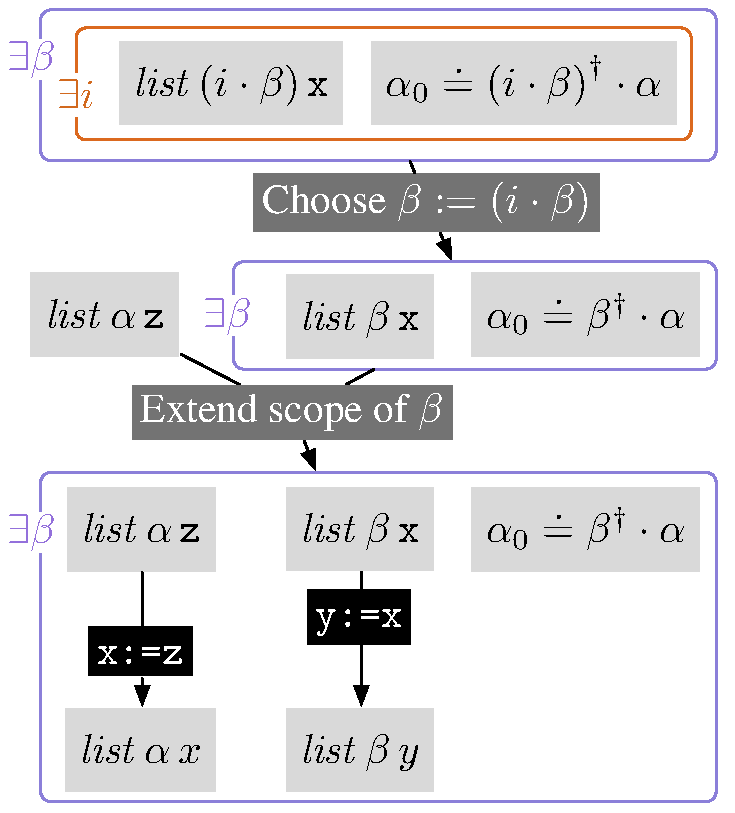
\includegraphics[width=57mm]{listrev_graph_new.pdf}
\else
\includegraphics[width=57mm]{listrev_graph_new_bw.pdf}
\fi
\hspace{-2mm}
\label{fig:listrev_graph}
\end{minipage}
}
\caption{Two ways to parse a fragment of Fig.~\ref{fig:listrev_proof_ribbon}}
\end{figure}

\noindent To illustrate how this syntax is used, Fig.~\ref{fig:listrev_fragment_stratified} shows a term of {\sf Diagram} that corresponds to a fragment of the picture in Fig.~\ref{fig:listrev_proof_ribbon}. Note that the cell in each row is always pushed to the left-hand side. In the concrete pictures, it can be moved to allow corresponding ribbons in different rows to be aligned, and hence for redundant labels to be removed. Each entailment $p⇒q$ is handled as the basic step $\seqspec{p}{\Skip}{q}$. Rather than write `$\Skip$', we label such a step with a justification of the entailment, and colour it dark grey to emphasise those steps that actually contain program instructions. Concerning existential boxes: the operations of extending, contracting and commuting are really the entailments depicted informally below. Having to show these entailments explicitly would make Fig.~\ref{fig:listrev_proof_ribbon} much more repetitive. (We are working on an improved formalisation that supports these operations directly -- see Sect.~\ref{sect:future} for further discussion.)
\begin{center}
\small $\begin{array}{rclrcl}
\begin{array}{@{}l@{}}
\begin{tikzpicture}[x=1mm,y=1mm,scale=1.]
\draw [rounded corners = 0.8mm, line width =0.15mm, \myblue] (12.15,0.) -- (12.15,0.);
\draw [rounded corners = 0.8mm, line width =0.15mm, \myblue] (20.85,0.) -- (20.85,0.);
\draw [rounded corners = 0.8mm, line width =0.15mm, \myblue] (12.15,-7.) -- (12.15,0.);
\draw [rounded corners = 0.8mm, line width =0.15mm, \myblue] (20.85,-7.) -- (20.85,0.);
\draw [line width = 0.5mm, white] (3.,0.) -- (3.,-7.);
\draw [line width = 0.5mm, white] (8.,0.) -- (8.,-7.);
\fill [black!15] (3.,0.) -- (3.,-7.) -- (8.,-7.) -- (8.,0.) -- cycle;
\draw [black] (5.5,-3.) node{\smash{$\ml[t]{p}$}};
\draw [line width = 0.5mm, white] (14.,0.) -- (14.,-7.);
\draw [line width = 0.5mm, white] (19.,0.) -- (19.,-7.);
\fill [black!15] (14.,0.) -- (14.,-7.) -- (19.,-7.) -- (19.,0.) -- cycle;
\draw [black] (16.5,-3.) node{\smash{$\ml[t]{q}$}};
\draw [line width = 0.5mm, white] (14.,-7.) -- (14.,-7.);
\draw [line width = 0.5mm, white] (19.,-7.) -- (19.,-7.);
\fill [black!15] (14.,-7.) -- (14.,-7.) -- (19.,-7.) -- (19.,-7.) -- cycle;
\draw [line width = 0.5mm, white] (3.,-7.) -- (3.,-7.);
\draw [line width = 0.5mm, white] (8.,-7.) -- (8.,-7.);
\fill [black!15] (3.,-7.) -- (3.,-7.) -- (8.,-7.) -- (8.,-7.) -- cycle;
\draw [rounded corners = 0.8mm, line width =0.15mm, \myblue] (12.15,-7.) -- (12.15,-7.);
\draw [rounded corners = 0.8mm, line width =0.15mm, \myblue] (20.85,-7.) -- (20.85,-7.);
\draw [line width = 0.5mm, white] (14.,-7.) -- (14.,-9.);
\draw [line width = 0.5mm, white] (19.,-7.) -- (19.,-9.);
\fill [black!15] (14.,-7.) -- (14.,-9.) -- (19.,-9.) -- (19.,-7.) -- cycle;
\draw [line width = 0.5mm, white] (3.,-7.) -- (3.,-9.);
\draw [line width = 0.5mm, white] (8.,-7.) -- (8.,-9.);
\fill [black!15] (3.,-7.) -- (3.,-9.) -- (8.,-9.) -- (8.,-7.) -- cycle;
\draw [rounded corners = 0.8mm, line width =0.15mm, \myblue] (1.15,-9.) -- (1.15,-8.) -- (12.15,-8.) -- (12.15,-7.);
\draw [rounded corners = 0.8mm, line width =0.15mm, \myblue] (20.85,-9.) -- (20.85,-7.);
\draw [line width = 0.5mm, white] (14.,-9.) -- (14.,-17.);
\draw [line width = 0.5mm, white] (19.,-9.) -- (19.,-17.);
\fill [black!15] (14.,-9.) -- (14.,-17.) -- (19.,-17.) -- (19.,-9.) -- cycle;
\draw [line width = 0.5mm, white] (3.,-9.) -- (3.,-17.);
\draw [line width = 0.5mm, white] (8.,-9.) -- (8.,-17.);
\fill [black!15] (3.,-9.) -- (3.,-17.) -- (8.,-17.) -- (8.,-9.) -- cycle;
\draw [rounded corners = 0.8mm, line width =0.15mm, \myblue] (1.15,-17.) -- (1.15,-9.);
\draw [rounded corners = 0.8mm, line width =0.15mm, \myblue] (20.85,-17.) -- (20.85,-9.);
\fill [white] (11.,-1.3) -- (11.,-4.8) -- (14.,-4.8) -- (14.,-1.3) -- cycle;
\draw [black] (8.,-3.) node[anchor=west,\myblue]{$∃x$};
\end{tikzpicture}
\end{array}
&~≝&\!\!\! 
\begin{array}{@{}l@{}}
\begin{tikzpicture}[x=1mm,y=1mm,scale=1.]
\draw [rounded corners = 0.8mm, line width =0.15mm, \myblue] (15.15,0.) -- (15.15,0.);
\draw [rounded corners = 0.8mm, line width =0.15mm, \myblue] (23.85,0.) -- (23.85,0.);
\draw [rounded corners = 0.8mm, line width =0.15mm, \myblue] (15.15,-5.) -- (15.15,0.);
\draw [rounded corners = 0.8mm, line width =0.15mm, \myblue] (23.85,-5.) -- (23.85,0.);
\draw [line width = 0.5mm, white] (3.,0.) -- (3.,-5.);
\draw [line width = 0.5mm, white] (8.,0.) -- (8.,-5.);
\fill [black!15] (3.,0.) -- (3.,-5.) -- (8.,-5.) -- (8.,0.) -- cycle;
\draw [black] (5.5,-3.) node{\smash{$\ml[t]{p}$}};
\draw [line width = 0.5mm, white] (17.,0.) -- (17.,-5.);
\draw [line width = 0.5mm, white] (22.,0.) -- (22.,-5.);
\fill [black!15] (17.,0.) -- (17.,-5.) -- (22.,-5.) -- (22.,0.) -- cycle;
\draw [black] (19.5,-3.) node{\smash{$\ml[t]{q}$}};
\draw [line width = 0.5mm, white] (17.,-5.) -- (17.,-5.);
\draw [line width = 0.5mm, white] (22.,-5.) -- (22.,-5.);
\fill [black!15] (17.,-5.) -- (17.,-5.) -- (22.,-5.) -- (22.,-5.) -- cycle;
\draw [line width = 0.5mm, white] (3.,-5.) -- (3.,-5.);
\draw [line width = 0.5mm, white] (8.,-5.) -- (8.,-5.);
\fill [black!15] (3.,-5.) -- (3.,-5.) -- (8.,-5.) -- (8.,-5.) -- cycle;
\draw [rounded corners = 0.8mm, line width =0.15mm, \myblue] (15.15,-5.) -- (15.15,-5.);
\draw [rounded corners = 0.8mm, line width =0.15mm, \myblue] (23.85,-5.) -- (23.85,-5.);
\draw [rounded corners = 0.8mm, line width =0.15mm, \myblue] (15.15,-6.) -- (15.15,-5.);
\draw [rounded corners = 0.8mm, line width =0.15mm, \myblue] (23.85,-6.) -- (23.85,-5.);
\draw [line width = 0.5mm, white] (17.,-5.) -- (17.,-6.);
\draw [line width = 0.5mm, white] (22.,-5.) -- (22.,-6.);
\fill [black!15] (17.,-5.) -- (17.,-6.) -- (22.,-6.) -- (22.,-5.) -- cycle;
\draw [line width = 0.5mm, white] (3.,-5.) -- (3.,-6.);
\draw [line width = 0.5mm, white] (8.,-5.) -- (8.,-6.);
\fill [black!15] (3.,-5.) -- (3.,-6.) -- (8.,-6.) -- (8.,-5.) -- cycle;
\fill[fill=black!55] (1.,-11.) rectangle (24.,-6.);
\draw [white] (1.,-8.5) node[anchor=west]{\begin{tabular}{@{\hspace{-0.8mm}}l@{\hspace{-0.8mm}}}Extend $x$'s scope\end{tabular}};
\draw [rounded corners = 0.8mm, line width =0.15mm, \myblue] (1.15,-11.) -- (1.15,-11.);
\draw [rounded corners = 0.8mm, line width =0.15mm, \myblue] (23.85,-11.) -- (23.85,-11.);
\draw [rounded corners = 0.8mm, line width =0.15mm, \myblue] (1.15,-11.) -- (1.15,-11.);
\draw [rounded corners = 0.8mm, line width =0.15mm, \myblue] (23.85,-11.) -- (23.85,-11.);
\draw [rounded corners = 0.8mm, line width =0.15mm, \myblue] (1.15,-17.) -- (1.15,-11.);
\draw [rounded corners = 0.8mm, line width =0.15mm, \myblue] (23.85,-17.) -- (23.85,-11.);
\draw [line width = 0.5mm, white] (3.,-11.) -- (3.,-17.);
\draw [line width = 0.5mm, white] (8.,-11.) -- (8.,-17.);
\fill [black!15] (3.,-11.) -- (3.,-17.) -- (8.,-17.) -- (8.,-11.) -- cycle;
\draw [black] (5.5,-14.) node{\smash{$\ml[t]{p}$}};
\draw [line width = 0.5mm, white] (17.,-11.) -- (17.,-17.);
\draw [line width = 0.5mm, white] (22.,-11.) -- (22.,-17.);
\fill [black!15] (17.,-11.) -- (17.,-17.) -- (22.,-17.) -- (22.,-11.) -- cycle;
\draw [black] (19.5,-14.) node{\smash{$\ml[t]{q}$}};
\fill [white] (0.,-12.3) -- (0.,-15.8) -- (3.,-15.8) -- (3.,-12.3) -- cycle;
\draw [black] (-3.,-14.) node[anchor=west,\myblue]{$∃x$};
\fill [white] (14.,-1.3) -- (14.,-4.8) -- (17.,-4.8) -- (17.,-1.3) -- cycle;
\draw [black] (11.,-3.) node[anchor=west,\myblue]{$∃x$};
\end{tikzpicture}
\end{array} \begin{array}{l}\text{if $x$ is} \\ \text{not free} \\ \text{in $p$}
\end{array}
~~~~ &~~~~
\begin{array}{@{}l@{}}
\begin{tikzpicture}[x=1mm,y=1mm,scale=1.]
\draw [rounded corners = 0.8mm, line width =0.15mm, \myblue] (3.15,0.) -- (3.15,0.);
\draw [rounded corners = 0.8mm, line width =0.15mm, \myblue] (18.85,0.) -- (18.85,0.);
\draw [rounded corners = 0.8mm, line width =0.15mm, \myred] (8.15,0.) -- (8.15,0.);
\draw [rounded corners = 0.8mm, line width =0.15mm, \myred] (16.85,0.) -- (16.85,0.);
\draw [rounded corners = 0.8mm, line width =0.15mm, \myblue] (3.15,-7.) -- (3.15,0.);
\draw [rounded corners = 0.8mm, line width =0.15mm, \myblue] (18.85,-7.) -- (18.85,0.);
\draw [rounded corners = 0.8mm, line width =0.15mm, \myred] (8.15,-7.) -- (8.15,0.);
\draw [rounded corners = 0.8mm, line width =0.15mm, \myred] (16.85,-7.) -- (16.85,0.);
\draw [line width = 0.5mm, white] (10.,0.) -- (10.,-7.);
\draw [line width = 0.5mm, white] (15.,0.) -- (15.,-7.);
\fill [black!15] (10.,0.) -- (10.,-7.) -- (15.,-7.) -- (15.,0.) -- cycle;
\draw [black] (12.5,-3.) node{\smash{$\ml[t]{p}$}};
\draw [line width = 0.5mm, white] (10.,-7.) -- (10.,-7.);
\draw [line width = 0.5mm, white] (15.,-7.) -- (15.,-7.);
\fill [black!15] (10.,-7.) -- (10.,-7.) -- (15.,-7.) -- (15.,-7.) -- cycle;
\draw [rounded corners = 0.8mm, line width =0.15mm, \myblue] (3.15,-7.) -- (3.15,-7.);
\draw [rounded corners = 0.8mm, line width =0.15mm, \myblue] (18.85,-7.) -- (18.85,-7.);
\draw [rounded corners = 0.8mm, line width =0.15mm, \myred] (8.15,-7.) -- (8.15,-7.);
\draw [rounded corners = 0.8mm, line width =0.15mm, \myred] (16.85,-7.) -- (16.85,-7.);
\draw [line width = 0.5mm, white] (10.,-7.) -- (10.,-9.);
\draw [line width = 0.5mm, white] (15.,-7.) -- (15.,-9.);
\fill [black!15] (10.,-7.) -- (10.,-9.) -- (15.,-9.) -- (15.,-7.) -- cycle;
\draw [rounded corners = 0.8mm, line width =0.15mm, \myblue] (3.15,-9.) -- (3.15,-7.);
\draw [rounded corners = 0.8mm, line width =0.15mm, \myblue] (18.85,-9.) -- (18.85,-7.);
\draw [rounded corners = 0.8mm, line width =0.15mm, \myred] (1.15,-9.) -- (1.15,-8.) -- (8.15,-8.) -- (8.15,-7.);
\draw [rounded corners = 0.8mm, line width =0.15mm, \myred] (20.85,-9.) -- (20.85,-8.) -- (16.85,-8.) -- (16.85,-7.);
\draw [line width = 0.5mm, white] (10.,-9.) -- (10.,-16.);
\draw [line width = 0.5mm, white] (15.,-9.) -- (15.,-16.);
\fill [black!15] (10.,-9.) -- (10.,-16.) -- (15.,-16.) -- (15.,-9.) -- cycle;
\draw [rounded corners = 0.8mm, line width =0.15mm, \myred] (1.15,-16.) -- (1.15,-9.);
\draw [rounded corners = 0.8mm, line width =0.15mm, \myred] (20.85,-16.) -- (20.85,-9.);
\draw [rounded corners = 0.8mm, line width =0.15mm, \myblue] (3.15,-16.) -- (3.15,-9.);
\draw [rounded corners = 0.8mm, line width =0.15mm, \myblue] (18.85,-16.) -- (18.85,-9.);
\fill [white] (7.,-1.3) -- (7.,-4.8) -- (10.,-4.8) -- (10.,-1.3) -- cycle;
\draw [black] (4.,-3.) node[anchor=west,\myred]{$∃y$};
\fill [white] (2.,-1.3) -- (2.,-4.8) -- (5.,-4.8) -- (5.,-1.3) -- cycle;
\draw [black] (-1.,-3.) node[anchor=west,\myblue]{$∃x$};
\end{tikzpicture}
\end{array} 
&~≝&\!\!\!
\begin{array}{@{}l@{}}
\begin{tikzpicture}[x=1mm,y=1mm,scale=1.]
\draw [rounded corners = 0.8mm, line width =0.15mm, \myblue] (1.15,0.) -- (1.15,0.);
\draw [rounded corners = 0.8mm, line width =0.15mm, \myblue] (18.85,0.) -- (18.85,0.);
\draw [rounded corners = 0.8mm, line width =0.15mm, \myred] (8.15,0.) -- (8.15,0.);
\draw [rounded corners = 0.8mm, line width =0.15mm, \myred] (16.85,0.) -- (16.85,0.);
\draw [rounded corners = 0.8mm, line width =0.15mm, \myblue] (1.15,-5.) -- (1.15,0.);
\draw [rounded corners = 0.8mm, line width =0.15mm, \myblue] (18.85,-5.) -- (18.85,0.);
\draw [rounded corners = 0.8mm, line width =0.15mm, \myred] (8.15,-5.) -- (8.15,0.);
\draw [rounded corners = 0.8mm, line width =0.15mm, \myred] (16.85,-5.) -- (16.85,0.);
\draw [line width = 0.5mm, white] (10.,0.) -- (10.,-5.);
\draw [line width = 0.5mm, white] (15.,0.) -- (15.,-5.);
\fill [black!15] (10.,0.) -- (10.,-5.) -- (15.,-5.) -- (15.,0.) -- cycle;
\draw [black] (12.5,-3.) node{\smash{$\ml[t]{p}$}};
\draw [line width = 0.5mm, white] (10.,-5.) -- (10.,-5.);
\draw [line width = 0.5mm, white] (15.,-5.) -- (15.,-5.);
\fill [black!15] (10.,-5.) -- (10.,-5.) -- (15.,-5.) -- (15.,-5.) -- cycle;
\draw [rounded corners = 0.8mm, line width =0.15mm, \myblue] (1.15,-5.) -- (1.15,-5.);
\draw [rounded corners = 0.8mm, line width =0.15mm, \myblue] (18.85,-5.) -- (18.85,-5.);
\draw [rounded corners = 0.8mm, line width =0.15mm, \myred] (8.15,-5.) -- (8.15,-5.);
\draw [rounded corners = 0.8mm, line width =0.15mm, \myred] (16.85,-5.) -- (16.85,-5.);
\draw [rounded corners = 0.8mm, line width =0.15mm, \myblue] (1.15,-6.) -- (1.15,-5.);
\draw [rounded corners = 0.8mm, line width =0.15mm, \myblue] (18.85,-6.) -- (18.85,-5.);
\draw [rounded corners = 0.8mm, line width =0.15mm, \myred] (8.15,-6.) -- (8.15,-5.);
\draw [rounded corners = 0.8mm, line width =0.15mm, \myred] (16.85,-6.) -- (16.85,-5.);
\draw [line width = 0.5mm, white] (10.,-5.) -- (10.,-6.);
\draw [line width = 0.5mm, white] (15.,-5.) -- (15.,-6.);
\fill [black!15] (10.,-5.) -- (10.,-6.) -- (15.,-6.) -- (15.,-5.) -- cycle;
\fill[fill=black!55] (1.,-10.) rectangle (19.,-6.);
\draw [white] (1.,-8.) node[anchor=west]{\begin{tabular}{@{\hspace{-0.8mm}}l@{\hspace{-0.8mm}}}Swap $x$ and $y$\end{tabular}};
\draw [rounded corners = 0.8mm, line width =0.15mm, \myblue] (8.15,-10.) -- (8.15,-10.);
\draw [rounded corners = 0.8mm, line width =0.15mm, \myblue] (16.85,-10.) -- (16.85,-10.);
\draw [rounded corners = 0.8mm, line width =0.15mm, \myred] (1.15,-10.) -- (1.15,-10.);
\draw [rounded corners = 0.8mm, line width =0.15mm, \myred] (18.85,-10.) -- (18.85,-10.);
\draw [rounded corners = 0.8mm, line width =0.15mm, \myblue] (8.15,-10.) -- (8.15,-10.);
\draw [rounded corners = 0.8mm, line width =0.15mm, \myblue] (16.85,-10.) -- (16.85,-10.);
\draw [rounded corners = 0.8mm, line width =0.15mm, \myred] (1.15,-10.) -- (1.15,-10.);
\draw [rounded corners = 0.8mm, line width =0.15mm, \myred] (18.85,-10.) -- (18.85,-10.);
\draw [rounded corners = 0.8mm, line width =0.15mm, \myblue] (8.15,-10.) -- (8.15,-10.);
\draw [rounded corners = 0.8mm, line width =0.15mm, \myblue] (16.85,-10.) -- (16.85,-10.);
\draw [rounded corners = 0.8mm, line width =0.15mm, \myred] (1.15,-10.) -- (1.15,-10.);
\draw [rounded corners = 0.8mm, line width =0.15mm, \myred] (18.85,-10.) -- (18.85,-10.);
\draw [rounded corners = 0.8mm, line width =0.15mm, \myblue] (8.15,-16.) -- (8.15,-10.);
\draw [rounded corners = 0.8mm, line width =0.15mm, \myblue] (16.85,-16.) -- (16.85,-10.);
\draw [rounded corners = 0.8mm, line width =0.15mm, \myred] (1.15,-16.) -- (1.15,-10.);
\draw [rounded corners = 0.8mm, line width =0.15mm, \myred] (18.85,-16.) -- (18.85,-10.);
\draw [line width = 0.5mm, white] (10.,-10.) -- (10.,-16.);
\draw [line width = 0.5mm, white] (15.,-10.) -- (15.,-16.);
\fill [black!15] (10.,-10.) -- (10.,-16.) -- (15.,-16.) -- (15.,-10.) -- cycle;
\draw [black] (12.5,-13.) node{\smash{$\ml[t]{p}$}};
\fill [white] (7.,-11.3) -- (7.,-14.8) -- (10.,-14.8) -- (10.,-11.3) -- cycle;
\draw [black] (4.,-13.) node[anchor=west,\myblue]{$∃x$};
\fill [white] (0.,-11.3) -- (0.,-14.8) -- (3.,-14.8) -- (3.,-11.3) -- cycle;
\draw [black] (-3.,-13.) node[anchor=west,\myred]{$∃y$};
\fill [white] (7.,-1.3) -- (7.,-4.8) -- (10.,-4.8) -- (10.,-1.3) -- cycle;
\draw [black] (4.,-3.) node[anchor=west,\myred]{$∃y$};
\fill [white] (0.,-1.3) -- (0.,-4.8) -- (3.,-4.8) -- (3.,-1.3) -- cycle;
\draw [black] (-3.,-3.) node[anchor=west,\myblue]{$∃x$};
\end{tikzpicture}
\end{array}
\end{array}$
\end{center}

\subsection{Proof rules for diagrams}\label{sect:formalisation_proofrules}

There are two pertinent questions to be asked of a given ribbon diagram. The first question is: is it a valid proof? This subsection develops a \emph{provability} judgement to answer this. The second question -- if this ribbon diagram \emph{is} deemed valid, what does it prove? -- is addressed in the next subsection.

\begin{figure}[t]
\newcommand{\myscale}[1]{\scalebox{1}{#1}}
\begin{mathpar}
\inferrule[Ribbon]
{ }{\Prov{\rm cel} P : P → P}
\and
\inferrule[Basic]
{\prov[SL]\{\assn P\}\,c\,\{\assn Q\}}
{\Prov{\rm cel} \basicstep{P}{c}{Q} : P → Q}
\and
\inferrule[Exists]
{\Prov{\rm dia} D : P → Q}
{\Prov{\rm cel} \existsbox{x}{D} \,:\! \existsbox{x}{P} \,→\! \existsbox{x}{Q}}
\vspace{-8mm}\\
\inferrule[Choice]
{\Prov{\rm dia} D : P → Q \\\\ \Prov{\rm dia} E : P → Q}
{\Prov{\rm cel} \choicedia{P}{D}{E}{Q} : P → Q}
\and
\inferrule[Loop]
{\Prov{\rm dia} D : P → P }
{\Prov{\rm cel} \loopdia{P}{D}{P} : P → P }
\and
\begin{minipage}{40mm}
\begin{mathpar}
\inferrule[Row]{\Prov{\rm cel} γ : P → Q \\ \WR(γ) ∩ \RD(F) = ∅}{\Prov{\rm row} (γ,F) : P ⊗ F → Q ⊗ F}
\and 
\inferrule[Main]
{\mbox{$\begin{array}{@{}l@{}}∀i≤k.\Prov{\rm row} ρ_i: P_i → P_{i+1}\end{array}$}}
{\Prov{\rm dia} [ρ_0,\dots,ρ_k] : P_0 → P_{k+1}}
\end{mathpar}
\end{minipage}
\end{mathpar}
\vspace{-7mm}
\caption{Proof rules for stratified ribbon diagrams}
\label{fig:rasterised_proof_rules}
\end{figure}

The rules given in Fig.~\ref{fig:rasterised_proof_rules} define provability judgements for cells ($\Prov{\rm cel}$), for rows ($\Prov{\rm row}$) and for diagrams ($\Prov{\rm dia}$). Each judgement ascribes a type, which comprises the top and bottom interfaces of that object.

The {\sc Row} and {\sc Main} rules recall Hoare logic's sequencing rule and separation logic's frame rule. They embody the `locally checkable' nature of ribbon proofs: that the entire diagram is valid if each row is valid in isolation, and that a row is valid if its active cell is valid and writes no program variable that is read elsewhere in the row.

The {\sc Basic} rule corresponds to an ordinary separation logic judgement $\prov[SL]\{p\}\,c\,\{q\}$. This judgement may be arbitrarily complex, so a ribbon diagram may be no easier to check than a traditional proof outline. This is intentional. Our formalisation \emph{allows} $p$ and $q$ to be minimised, by framing common fragments away, but does not \emph{demand} this. The command $c$ \emph{can} be reduced to $\Skip$ or some primitive command, but this may not be desirable if one requires only a high-level overview proof. A ribbon diagram can thus be viewed as a flexible combination of diagrammatic and traditional proofs, with the {\sc Basic} rule as the interface between these two levels.

We remark that these proof rules provide only limited mechanisms for building new diagrams from old. Diagrams can be wrapped in existential boxes, or put inside choice or loop diagrams, but not stacked vertically or placed side by side. One can define operations for composing elements of {\sf Diagram} in sequence or in parallel, and hence additional proof rules for diagrams so composed. The process is straightforward, and described in Wickerson's PhD dissertation~\cite{wickerson13}.

\subsection{Semantics of diagrams}\label{sect:formalisation_semantics}

\begin{figure}[t] 
\begin{mathpar}
\begin{array}[t]{@{}l@{}}\COM [(γ_0,F_0), \dots, (γ_k,F_k)] {}\\~~~~~{} = \COM γ_0 \mathbin{\code{;}} \cdots \mathbin{\code{;}} \COM γ_k\end{array}
\hspace{-6mm}\and
\COM P ~=~ \Skip
\hspace{-6mm}\and
\COM \existsbox{x}{D} ~= \COM {D}
\vspace{-5mm}\\
\COM \basicstep{P}{c}{Q} ~=~ c
\and
\COM \loopdia{P}{D}{Q} ~=~ \mathop{\code{loop}} (\COM {D})
\and
\raisebox{2mm}{\ensuremath{\COM \choicedia{P}{D}{E}{Q} ~=~ \begin{array}[t]{@{}l@{}}(\COM {D}) \\ \mathbin{\code{or}} (\COM {E})\end{array}}}
\end{mathpar}
\vspace{-5mm}
\caption{Extracting a command from a stratified diagram}
\label{fig:com_function}
\end{figure}

A stratified ribbon diagram denotes a Hoare triple. The pre- and postconditions of this triple are the assertions represented by the diagram's top and bottom interfaces. The command being proved is extracted by composing the labels on all of the proof steps in top-to-bottom order. Figure~\ref{fig:com_function} defines the function responsible for this extraction. We hence obtain the following soundness result for ribbon proofs.

\begin{theorem}[Soundness -- stratified diagrams]\label{thm:soundness_rasterised} Separation logic can encode any provable ribbon diagram.
\begin{eqnarray*}
\Prov{\rm dia} D:P→Q &⟹& \prov[SL]\{ \assn P \}\,\COM {D}\,\{ \assn Q \}.
\end{eqnarray*}
\end{theorem}
\begin{proof}
\renewcommand{\squareforqed}{\hbox{\rlap{$\isabelle$}$\isabelle$}}
By mutual rule induction on $\Prov{\rm cel}$, $\Prov{\rm row}$, and $\Prov{\rm dia}$.\qed
\end{proof}

\noindent Ribbon diagrams are trivially complete, because the {\sc Basic} rule can be invoked right at the root of the proof tree. In fact, ribbon diagrams remain complete even when the {\sc Basic} rule can occur only immediately beneath an axiom or the rule of consequence.

\begin{theorem}[Completeness -- stratified diagrams]\label{thm:completeness} A strengthened ribbon proof system in which the {\sc Basic} rule is replaced by
\[
\small
\inferrule
{(\assn P,c,\assn Q)∈{\sf Axioms}}
{\Prov{\rm cel} \basicstep{P}{c}{Q} : P → Q}
\hspace{5mm}\text{\normalsize and}\hspace{5mm}
\inferrule
{\assn P ⇒ \assn Q}
{\Prov{\rm cel} \basicstep{P}{{\mbox{\upshape\Skip}}}{Q} : P → Q}
\]
can encode any separation logic proof. 
\begin{eqnarray*}
\prov[SL]\{p\}\,c\,\{q\} &⟹& 
∃D,P,Q.c \!∈\! \COM D ∧ p \!=\! \assn P ∧ q \!=\! \assn Q ∧ \Prov{\rm dia} D : P\!→\!Q
\end{eqnarray*}
\end{theorem}
\begin{proof}
By rule induction on $\prov[SL]$.\qed
\end{proof}

\noindent The main problem with the formalisation given in this section is that it sacrifices much of the flexibility we expect in our ribbon diagrams. It is often sound to tweak the layout of a diagram by sliding steps up or down or reordering ribbons, but by thinking of our diagrams as sliced into a sequence of rows, we rule out \emph{all} such manoeuvres.

\section{Graphical formalisation}\label{sect:v_a_r}

We now give an alternative formalisation, in which diagrams are represented not as a sequence of rows, but as graphs. 

Our `graphical' diagrams are more flexible than their `stratified' cousins, but extra precautions must be taken to ensure soundness. The core difficulty is the side-condition on the frame rule: that the command writes no program variable in the frame. With stratification, the frame is clearly delimited, so this condition is easily checked. Without it, this check would become more global: a command may affect a ribbon that appears far above or below itself in a laid-out diagram. Our simple solution is to require henceforth that the frame rule has no side-condition. This requirement could be met by abolishing program variables altogether, leaving only the heap and numerical constants. A more practical alternative, explored later in this section, is to use the \emph{variables-as-resource} paradigm~\cite{bornat+06}.

Our graphs are nested, directed, acyclic hypergraphs. Ribbons correspond to nodes, and basic steps to hyperedges. Existential boxes are represented as single nodes that contain a nested graph. Likewise, choice diagrams and loop diagrams are represented by single hyperedges that contain, respectively, one or two nested graphs.

\newcommand{\filledarrowright}{\mathrel{{-}\!\raisebox{0.4mm}{\scalebox{.5}{$\blacktriangleright$}}}}

\begin{definition}[Graphical diagrams, assertion-gadgets and command-gadgets]\label{defn:diagrams}
Let $\mathcal V$ be an infinite set of node-identifiers. We define a language of \emph{assertion-gadgets}, \emph{command-gadgets} and \emph{graphical diagrams} as follows.
\vspace{-3mm}
\begin{center}
\small
${\sf AsnGadget} ~=~ \{A ::= \closedribbon{p} \mid \closedexistsbox{x}{\,G\,}\}
~~~~~~~~
{\sf ComGadget} ~=~ \{C ::= \nakedbasicstep{c} \mid \nakedchoicedia{G}{G} \mid \nakedloopdia{G}\,\}$
\\
${\sf GDiagram} ~=~ {\begin{array}[t]{@{}l@{}l@{}}\{G \mid {} & \text{$Λ_G ∈ V_G → {\sf AsnGadget}$, $E_G ⊆_{\rm fin} \pow(V_G) × {\sf ComGadget} × \pow(V_G)$,} \\ & \text{$V_G ⊆_{\rm fin} \mathcal V$, $\acyclic(G)$ and $\linear(G)$, where $G = (V_G,Λ_G,E_G)$}\}\end{array}}$
\end{center}
The definitions are mutually recursive, and are well-formed because the definienda (left-hand sides) appear only positively in the definientia (right-hand sides).\footnote{This is true even for the occurrence of {\sf ComGadget} in the definiens of {\sf GDiagram}, because the set in which it appears is finite.} The first of these equations defines an assertion-gadget $A ∈ {\sf AsnGadget}$ to be either a ribbon or an existential box. The second defines a command-gadget $C ∈ {\sf ComGadget}$ to be either a basic step, a choice diagram, or a loop diagram. The third equation defines a graphical diagram $G ∈ {\sf GDiagram}$ to be a triple $(V_G,Λ_G,E_G)$ that comprises:
\begin{itemize} 
\item a finite set $V_G ⊆_{\rm fin} \mathcal V$ of \emph{node identifiers};
\item a \emph{labelling} $Λ_G : V_G → {\sf AsnGadget}$ that associates each node identifier with an assertion-gadget; and 
\item a finite set $E_G ⊆_{\rm fin} \pow(V_G) × {\sf ComGadget} × \pow(V_G)$ of \emph{hyperedges} $(\bold v,C,\bold w)$, each comprising a set $\bold v$ of tail identifiers, a command-gadget $C$, and a set $\bold w$ of head identifiers,
\end{itemize} 
and which satisfies the following two properties.
\begin{description}
\item[{\sc Acyclicity:}] Let us write $v \filledarrowright w$ if $v∈\bold v$ and $w∈\bold w$ for some $(\bold v,C,\bold w)∈E_G$. Then define $\acyclic(G)$ to hold iff the transitive closure of $\filledarrowright$ is irreflexive.
\item[{\sc Linearity:}] Define $\linear(G)$ to hold iff the hyperedges in $E_G$ have no common heads and no common tails. (This forbids the duplication or merging of ribbons, in accordance with $p ⇒ p*p$ and $p*p ⇒ p$ being invalid in separation logic.)
\end{description}
\end{definition}

\begin{remark}
We could represent our diagrams by a single graph, with dedicated `parent' edges to simulate the nesting hierarchy. However, mindful of our \emph{Isabelle} formalisation, and that ``reasoning about graphs [\dots] can be a real hassle in HOL-based theorem provers''~\cite{wu+11}, we prefer to use an algebraic datatype to depict the hierarchy.
\end{remark}

\noindent Figure~\ref{fig:listrev_graph} presents a term of {\sf GDiagram} that corresponds to a fragment of the picture in Fig.~\ref{fig:listrev_proof_ribbon}. Unlike Fig.~\ref{fig:listrev_fragment_stratified}, this representation does not impose a strict ordering between the `\code{y:=x}' and `\code{x:=z}' instructions. As such, this proof is \emph{invalid}; the figure serves merely to demonstrate how the graphical syntax is used. 

The problem is that the graph does not take into account dependencies on program variables. To address this, let us remove the side-condition on the frame rule in our axiomatisation $\prov[SL]$ of separation logic (Fig.~\ref{fig:prov_com}). The new proof system thus obtained shall be written as $\Prov[SL]{*}$. We shall now develop proof rules for graphical diagrams, and show them to be sound and complete with respect to $\Prov[SL]{*}$. Section~\ref{sect:using_var} describes the application of ribbon proofs to variables-as-resource, which is one instance of $\Prov[SL]{*}$.

\subsection{Proof rules for graphical diagrams}

Proof rules for graphical diagrams, command-gadgets and assertion-gadgets are defined in Fig.~\ref{fig:proof_rules}, which refers to the $\TOP$ and $\BOT$ functions defined below. The judgement $\Prov{\rm gra} G : P → Q$ means that the diagram $G$, precondition $P$, and postcondition $Q$ form a valid proof. The interfaces $P$ and $Q$ are always equal to $\TOP(G)$ and $\BOT(G)$ respectively, so we sometimes omit them. The judgements for command-gadgets and assertion-gadgets are similar, the latter without interfaces. 

\begin{definition}[Top and bottom interfaces]\label{defn:top_bot}
These functions extract interfaces from assertion-gadgets and from diagrams. For assertion-gadgets:
\begin{mathpar}
\TOP \closedribbon p = \ribbon p\!\!\!
\and
\BOT \closedribbon p = \ribbon p\!\!\!
\and
\TOP \closedexistsbox{x}{G} = \existsbox{x}{\TOP G}\!\!\!
\and
\BOT \closedexistsbox{x}{G} = \existsbox{x}{\BOT G}\,.
\end{mathpar} 
For diagrams:
\begin{mathpar}
\TOP(G) ~=~ ⊗_{v∈\initials G}\TOP(Λ_G\,v)
\and
\BOT(G) ~=~ ⊗_{v∈\terminals G}\BOT(Λ_G\,v)
\end{mathpar}
where $\initials(G) = V_G \setminus \bigcup_{(\_,\_,\bold v)∈E_G} \bold v$ and $\terminals(G) = V_G \setminus \bigcup_{(\bold v,\_,\_)∈E_G} \bold v$.
\end{definition}

\begin{figure}[t]
\begin{mathpar}
\inferrule[GRibbon]
{ }{\Prov{\rm asn} \closedribbon{p} %: \ribbon{p} → \ribbon{p}
}
\and
\inferrule[GBasic]
{\Prov[SL]{*}\{\assn P\}\,c\,\{\assn Q\}}
{
\Prov{\rm com} \nakedbasicstep{c} : P → Q
}
\and
\inferrule[GExists]
{\Prov{\rm gra} G %: P → Q
}
{\Prov{\rm asn} \closedexistsbox{x}{G} %: \existsbox{x}{P} → \existsbox{x}{Q}
}
\and
\inferrule[GChoice]
{\Prov{\rm gra} G_1 : P → Q \\\\ \Prov{\rm gra} G_2 : P → Q}
{\Prov{\rm com} \nakedchoicedia{G_1}{G_2} : P → Q}
\vspace{-5mm}\\
\inferrule[GLoop]
{\Prov{\rm gra} G : P → P}
{\Prov{\rm com} \nakedloopdia[9]{G} : P → P }
\hspace{-5mm}\and
\inferrule[GMain]
{∀v∈V_G.\Prov{\rm asn} Λ_G\,v %: \TOP (Λ_G\,v) → \BOT (Λ_G\,v) 
\\\\
∀(\bold v,C,\bold w)∈E_G.\Prov{\rm com} C : ⊗_{v∈\bold v}\BOT(Λ_G\,v) → ⊗_{w∈\bold w}\TOP(Λ_G\,w)
}
{\Prov{\rm gra} G : \TOP(G) → \BOT(G)}
\end{mathpar}
\vspace{-5mm}
\caption{Proof rules for graphical diagrams}
\label{fig:proof_rules}
\end{figure}

\noindent As was the case for stratified diagrams, one can define operations for composing elements of {\sf GDiagram} in sequence or parallel, and hence additional proof rules for graphical diagrams so composed~\cite{wickerson13}.

\subsection{Semantics of graphical diagrams}

Since graphical diagrams have a parallel nature, but our language is only sequential, it follows that each graphical diagram proves not a single command, but a set of commands, each one a linear extension of the partial order imposed by the diagram. The $\mathit{coms}$ function defined in Fig.~\ref{fig:coms_function} is responsible for extracting this set from a given diagram. Each command is obtained by picking an ordering of command- and assertion-gadgets that is compatible with the partial order defined by the edges (this is the purpose of the $\lin$ function defined below), then recursively extracting a command from each gadget and sequentially composing the results.

\begin{definition}[Linear extensions]
For a diagram $G$, we define $\lin G$ as the set of all lists $[x_0,\dots,x_{k-1}]$ of {\sf AsnGadget}s and {\sf ComGadget}s, for which there exists a bijection $π: k → V_G ∪ E_G$ that satisfies, for all $(\bold v,C,\bold w)∈E_G$: 
\begin{mathpar}
∀v∈\bold v.π^{-1}(v) < π^{-1}(\bold v,C,\bold w)
\and
∀w∈\bold w.π^{-1}(\bold v,C,\bold w) < π^{-1}(w)
\end{mathpar}
and where, for all $i<k$: $x_i = Λ_G(v)$ if $π(i)=v$, and $x_i = C$ if $π(i) = (\bold v,C,\bold w)$.
% \[
% x_i = \begin{cases} Λ_G(v) & \text{if $π(i)=v$} \\ C & \text{if $π(i) = (\bold v,C,\bold w)$}. \end{cases}
% \]
\end{definition}

\noindent By {\sc Acyclicity}, every diagram admits at least one linear extension.

\begin{figure}[t]
\begin{mathpar}
\coms(G) ~=~ \{c_0\Semicolon\cdots\Semicolon c_{k-1} \Semicolon \Skip \mid ∃[x_0,\dots,x_{k-1}] ∈ \lin G.∀i<k.c_i ∈ \coms x_i \}
\and
\coms {\closedribbon{p}} ~=~ \{\Skip\}
\and
\coms {\closedexistsbox{x}{G}} ~=~ \coms{G}
\and
\coms {\nakedbasicstep{c}} ~=~ \{c\}
\and
\coms {\nakedchoicedia{G_1}{G_2}} ~=~ \begin{array}{@{}l@{}l@{}} \{ & c_1 \mathbin{\code{or}} c_2 \mid \\ & c_1 ∈ \coms G_1, \\ & c_2 ∈ \coms G_2\} \end{array}
\and
\coms {\nakedloopdia{G}} ~=~ \{\mathop{\code{loop}} c \mid c ∈ \coms G\}
\end{mathpar}
\vspace{-2mm}
\caption{Extracting commands from a diagram}
\label{fig:coms_function}
\end{figure}

\begin{theorem}[Soundness -- graphical diagrams]\label{thm:soundness3}
Separation logic without the side-condition on the frame rule can encode any provable ribbon diagram:
\begin{eqnarray*}
\Prov{\rm gra} G:P→Q &⟹& ∀c∈\coms G.\Prov[SL]{*} \{\assn P\}\,c\,\{\assn Q\}.
\end{eqnarray*}
\end{theorem}
\begin{proof}
\renewcommand{\squareforqed}{\hbox{\rlap{$\isabelle$}$\isabelle$}}
By mutual induction on $\Prov{\rm gra}$, $\Prov{\rm com}$ and $\Prov{\rm dia}$. See~\cite{wickerson13} for details.\qed
\end{proof}


\begin{theorem}[Completeness -- graphical diagrams]\label{thm:completeness} A strengthened ribbon proof system in which the {\sc GBasic} rule is replaced by
\begin{center}
\small $\inferrule
{(\assn P,c,\assn Q)∈{\sf Axioms}}
{
\Prov{\rm com} \nakedbasicstep{c} : P → Q
}$
\hspace{5mm}\text{\normalsize and}\hspace{5mm}
$\inferrule
{\assn P ⇒ \assn Q}
{
\Prov{\rm com} \nakedbasicstep{\mbox{\rm \Skip}} : P → Q
}$
\end{center}
can encode any proof in separation logic without the side-condition on the frame rule. 
\begin{eqnarray*}
\Prov[SL]{*}\{p\}\,c\,\{q\} &\,⟹\,& ∃G,P,Q.c\!∈\!\coms G ∧ p\!=\!\assn P ∧ q\!=\!\assn Q ∧ \Prov{\rm gra} G : P\!→\!Q
\end{eqnarray*}
\end{theorem}
\begin{proof}
By rule induction on $\Prov[SL]{*}$.\qed
\end{proof}

\begin{figure}[tp]
\centering
%Starting.
\pgfdeclarelayer{frontmost}
\pgfdeclarelayer{colnameslayer}
\pgfsetlayers{main,frontmost,colnameslayer}
\begin{tikzpicture}[x=1mm,y=1mm,scale=0.83]
% State has been set.
\draw [line width = 0.5mm, white] (42.,0.) -- (42.,-6.);
\draw [line width = 0.5mm, white] (64.,0.) -- (64.,-6.);
\fill [black!15] (42.,0.) -- (42.,-6.) -- (64.,-6.) -- (64.,0.) -- cycle;
\fill [black!21] (42.,0.) -- (42.,-6.) -- (49.,-6.) -- (49.,0.) -- cycle;
\begin{pgfonlayer}{frontmost}
\draw [black] (56.5,-4.) node{\smash{$\ml[t]{\List{α_0}{\code x}}$}};
\end{pgfonlayer}
\begin{pgfonlayer}{frontmost}
\draw [black] (45.5,-4.) node{\smash{$\ml[t]{\code{x}}$}};
\end{pgfonlayer}
\draw [line width = 0.5mm, white] (79.,0.) -- (79.,-6.);
\draw [line width = 0.5mm, white] (86.,0.) -- (86.,-6.);
\fill [black!15] (79.,0.) -- (79.,-6.) -- (86.,-6.) -- (86.,0.) -- cycle;
\fill [black!21] (79.,0.) -- (79.,-6.) -- (86.,-6.) -- (86.,0.) -- cycle;
\begin{pgfonlayer}{frontmost}
\draw [black] (82.5,-4.) node{\smash{$\ml[t]{\code{y}}$}};
\end{pgfonlayer}
\draw [line width = 0.5mm, white] (66.,0.) -- (66.,-6.);
\draw [line width = 0.5mm, white] (73.,0.) -- (73.,-6.);
\fill [black!15] (66.,0.) -- (66.,-6.) -- (73.,-6.) -- (73.,0.) -- cycle;
\fill [black!21] (66.,0.) -- (66.,-6.) -- (73.,-6.) -- (73.,0.) -- cycle;
\begin{pgfonlayer}{frontmost}
\draw [black] (69.5,-4.) node{\smash{$\ml[t]{\code{z}}$}};
\end{pgfonlayer}
\begin{pgfonlayer}{frontmost}
\fill[fill=black!55] (11.,-11.) rectangle (64.,-6.);
\draw [white] (11.,-8.5) node[anchor=west]{\begin{tabular}{@{\hspace{-0.8mm}}l@{\hspace{-0.8mm}}}Split \code{x}\end{tabular}};
\end{pgfonlayer}
\begin{pgfonlayer}{frontmost}
\fill[fill=black] (79.,-11.) rectangle (125.,-6.);
\draw [white] (79.,-8.5) node[anchor=west]{\code{\begin{tabular}{@{\hspace{-0.8mm}}l@{\hspace{-0.8mm}}}y:=nil\end{tabular}}};
\end{pgfonlayer}
\draw [line width = 0.5mm, white] (66.,-6.) -- (66.,-11.);
\draw [line width = 0.5mm, white] (73.,-6.) -- (73.,-11.);
\fill [black!15] (66.,-6.) -- (66.,-11.) -- (73.,-11.) -- (73.,-6.) -- cycle;
\fill [black!21] (66.,-6.) -- (66.,-11.) -- (73.,-11.) -- (73.,-6.) -- cycle;
\draw [line width = 0.5mm, white] (66.,-11.) -- (66.,-17.);
\draw [line width = 0.5mm, white] (73.,-11.) -- (73.,-17.);
\fill [black!15] (66.,-11.) -- (66.,-17.) -- (73.,-17.) -- (73.,-11.) -- cycle;
\fill [black!21] (66.,-11.) -- (66.,-17.) -- (73.,-17.) -- (73.,-11.) -- cycle;
\draw [line width = 0.5mm, white] (11.,-11.) -- (11.,-17.);
\draw [line width = 0.5mm, white] (21.,-11.) -- (21.,-17.);
\fill [black!15] (11.,-11.) -- (11.,-17.) -- (21.,-17.) -- (21.,-11.) -- cycle;
\fill [black!21] (11.,-11.) -- (11.,-17.) -- (21.,-17.) -- (21.,-11.) -- cycle;
\begin{pgfonlayer}{frontmost}
\draw [black] (16.,-15.) node{\smash{$\ml[t]{\frac12\code{x}}$}};
\end{pgfonlayer}
\draw [line width = 0.5mm, white] (42.,-11.) -- (42.,-17.);
\draw [line width = 0.5mm, white] (64.,-11.) -- (64.,-17.);
\fill [black!15] (42.,-11.) -- (42.,-17.) -- (64.,-17.) -- (64.,-11.) -- cycle;
\fill [black!21] (42.,-11.) -- (42.,-17.) -- (49.,-17.) -- (49.,-11.) -- cycle;
\begin{pgfonlayer}{frontmost}
\draw [black] (56.5,-15.) node{\smash{$\ml[t]{\List{α_0}{\code x}}$}};
\end{pgfonlayer}
\begin{pgfonlayer}{frontmost}
\draw [black] (45.5,-15.) node{\smash{$\ml[t]{\frac12\code{x}}$}};
\end{pgfonlayer}
\draw [line width = 0.5mm, white] (79.,-11.) -- (79.,-17.);
\draw [line width = 0.5mm, white] (125.,-11.) -- (125.,-17.);
\fill [black!15] (79.,-11.) -- (79.,-17.) -- (125.,-17.) -- (125.,-11.) -- cycle;
\fill [black!21] (79.,-11.) -- (79.,-17.) -- (86.,-17.) -- (86.,-11.) -- cycle;
\begin{pgfonlayer}{frontmost}
\draw [black] (105.5,-15.) node{\smash{$\ml[t]{\List{ε}{\code y}}$}};
\end{pgfonlayer}
\begin{pgfonlayer}{frontmost}
\draw [black] (82.5,-15.) node{\smash{$\ml[t]{\code y}$}};
\end{pgfonlayer}
\begin{pgfonlayer}{frontmost}
\fill[fill=black!55] (34.,-22.) rectangle (133.,-17.);
\draw [white] (34.,-19.5) node[anchor=west]{\begin{tabular}{@{\hspace{-0.8mm}}l@{\hspace{-0.8mm}}}Choose $α := α_0$ and $β := ε$\end{tabular}};
\end{pgfonlayer}
\draw [line width = 0.5mm, white] (11.,-17.) -- (11.,-22.);
\draw [line width = 0.5mm, white] (21.,-17.) -- (21.,-22.);
\fill [black!15] (11.,-17.) -- (11.,-22.) -- (21.,-22.) -- (21.,-17.) -- cycle;
\fill [black!21] (11.,-17.) -- (11.,-22.) -- (21.,-22.) -- (21.,-17.) -- cycle;
\draw [line width = 0.5mm, white] (66.,-17.) -- (66.,-22.);
\draw [line width = 0.5mm, white] (73.,-17.) -- (73.,-22.);
\fill [black!15] (66.,-17.) -- (66.,-22.) -- (73.,-22.) -- (73.,-17.) -- cycle;
\fill [black!21] (66.,-17.) -- (66.,-22.) -- (73.,-22.) -- (73.,-17.) -- cycle;
% Pen up
% Pen down
\draw [line width = 0.5mm, white] (11.,-22.) -- (11.,-22.);
\draw [line width = 0.5mm, white] (21.,-22.) -- (21.,-22.);
\fill [black!15] (11.,-22.) -- (11.,-22.) -- (21.,-22.) -- (21.,-22.) -- cycle;
\fill [black!21] (11.,-22.) -- (11.,-22.) -- (21.,-22.) -- (21.,-22.) -- cycle;
\draw [line width = 0.5mm, white] (66.,-22.) -- (66.,-22.);
\draw [line width = 0.5mm, white] (73.,-22.) -- (73.,-22.);
\fill [black!15] (66.,-22.) -- (66.,-22.) -- (73.,-22.) -- (73.,-22.) -- cycle;
\fill [black!21] (66.,-22.) -- (66.,-22.) -- (73.,-22.) -- (73.,-22.) -- cycle;
\draw [rounded corners = 0.8mm, line width =0.15mm, \mypurple] (40.15,-22.) -- (40.15,-22.);
\draw [rounded corners = 0.8mm, line width =0.15mm, \mypurple] (130.85,-22.) -- (130.85,-22.);
\draw [rounded corners = 0.8mm, line width =0.15mm, \mygreen] (34.15,-22.) -- (34.15,-22.);
\draw [rounded corners = 0.8mm, line width =0.15mm, \mygreen] (132.85,-22.) -- (132.85,-22.);
\begin{pgfonlayer}{frontmost}
\fill [white] (32.,-23.3) -- (32.,-26.8) -- (35.,-26.8) -- (35.,-23.3) -- cycle;
\end{pgfonlayer}
\begin{pgfonlayer}{frontmost}
\draw [black] (29.,-25.) node[anchor=west,\mygreen]{$∃α$};
\end{pgfonlayer}
\draw [line width = 0.5mm, white] (11.,-22.) -- (11.,-22.);
\draw [line width = 0.5mm, white] (21.,-22.) -- (21.,-22.);
\fill [black!15] (11.,-22.) -- (11.,-22.) -- (21.,-22.) -- (21.,-22.) -- cycle;
\fill [black!21] (11.,-22.) -- (11.,-22.) -- (21.,-22.) -- (21.,-22.) -- cycle;
\draw [line width = 0.5mm, white] (66.,-22.) -- (66.,-22.);
\draw [line width = 0.5mm, white] (73.,-22.) -- (73.,-22.);
\fill [black!15] (66.,-22.) -- (66.,-22.) -- (73.,-22.) -- (73.,-22.) -- cycle;
\fill [black!21] (66.,-22.) -- (66.,-22.) -- (73.,-22.) -- (73.,-22.) -- cycle;
\draw [rounded corners = 0.8mm, line width =0.15mm, \mypurple] (40.15,-22.) -- (40.15,-22.);
\draw [rounded corners = 0.8mm, line width =0.15mm, \mypurple] (130.85,-22.) -- (130.85,-22.);
\draw [rounded corners = 0.8mm, line width =0.15mm, \mygreen] (34.15,-22.) -- (34.15,-22.);
\draw [rounded corners = 0.8mm, line width =0.15mm, \mygreen] (132.85,-22.) -- (132.85,-22.);
\begin{pgfonlayer}{frontmost}
\fill [white] (38.,-23.3) -- (38.,-26.8) -- (41.,-26.8) -- (41.,-23.3) -- cycle;
\end{pgfonlayer}
\begin{pgfonlayer}{frontmost}
\draw [black] (35.,-25.) node[anchor=west,\mypurple]{$∃β$};
\end{pgfonlayer}
\draw [line width = 0.5mm, white] (11.,-22.) -- (11.,-22.);
\draw [line width = 0.5mm, white] (21.,-22.) -- (21.,-22.);
\fill [black!15] (11.,-22.) -- (11.,-22.) -- (21.,-22.) -- (21.,-22.) -- cycle;
\fill [black!21] (11.,-22.) -- (11.,-22.) -- (21.,-22.) -- (21.,-22.) -- cycle;
\draw [line width = 0.5mm, white] (66.,-22.) -- (66.,-22.);
\draw [line width = 0.5mm, white] (73.,-22.) -- (73.,-22.);
\fill [black!15] (66.,-22.) -- (66.,-22.) -- (73.,-22.) -- (73.,-22.) -- cycle;
\fill [black!21] (66.,-22.) -- (66.,-22.) -- (73.,-22.) -- (73.,-22.) -- cycle;
\draw [rounded corners = 0.8mm, line width =0.15mm, \mypurple] (40.15,-22.) -- (40.15,-22.);
\draw [rounded corners = 0.8mm, line width =0.15mm, \mypurple] (130.85,-22.) -- (130.85,-22.);
\draw [rounded corners = 0.8mm, line width =0.15mm, \mygreen] (34.15,-22.) -- (34.15,-22.);
\draw [rounded corners = 0.8mm, line width =0.15mm, \mygreen] (132.85,-22.) -- (132.85,-22.);
\draw [line width = 0.5mm, white] (66.,-22.) -- (66.,-28.);
\draw [line width = 0.5mm, white] (73.,-22.) -- (73.,-28.);
\fill [black!15] (66.,-22.) -- (66.,-28.) -- (73.,-28.) -- (73.,-22.) -- cycle;
\fill [black!21] (66.,-22.) -- (66.,-28.) -- (73.,-28.) -- (73.,-22.) -- cycle;
\draw [rounded corners = 0.8mm, line width =0.15mm, \mypurple] (40.15,-28.) -- (40.15,-22.);
\draw [rounded corners = 0.8mm, line width =0.15mm, \mypurple] (130.85,-28.) -- (130.85,-22.);
\draw [rounded corners = 0.8mm, line width =0.15mm, \mygreen] (34.15,-28.) -- (34.15,-22.);
\draw [rounded corners = 0.8mm, line width =0.15mm, \mygreen] (132.85,-28.) -- (132.85,-22.);
\draw [line width = 0.5mm, white] (11.,-22.) -- (11.,-28.);
\draw [line width = 0.5mm, white] (21.,-22.) -- (21.,-28.);
\fill [black!15] (11.,-22.) -- (11.,-28.) -- (21.,-28.) -- (21.,-22.) -- cycle;
\fill [black!21] (11.,-22.) -- (11.,-28.) -- (21.,-28.) -- (21.,-22.) -- cycle;
\draw [line width = 0.5mm, white] (42.,-22.) -- (42.,-28.);
\draw [line width = 0.5mm, white] (64.,-22.) -- (64.,-28.);
\fill [black!15] (42.,-22.) -- (42.,-28.) -- (64.,-28.) -- (64.,-22.) -- cycle;
\fill [black!21] (42.,-22.) -- (42.,-28.) -- (49.,-28.) -- (49.,-22.) -- cycle;
\begin{pgfonlayer}{frontmost}
\draw [black] (56.5,-26.) node{\smash{$\ml[t]{\List{α}{\code x}}$}};
\end{pgfonlayer}
\begin{pgfonlayer}{frontmost}
\draw [black] (45.5,-26.) node{\smash{$\ml[t]{\frac12\code{x}}$}};
\end{pgfonlayer}
\draw [line width = 0.5mm, white] (79.,-22.) -- (79.,-28.);
\draw [line width = 0.5mm, white] (102.,-22.) -- (102.,-28.);
\fill [black!15] (79.,-22.) -- (79.,-28.) -- (102.,-28.) -- (102.,-22.) -- cycle;
\fill [black!21] (79.,-22.) -- (79.,-28.) -- (86.,-28.) -- (86.,-22.) -- cycle;
\begin{pgfonlayer}{frontmost}
\draw [black] (94.,-26.) node{\smash{$\ml[t]{\List{β}{\code y}}$}};
\end{pgfonlayer}
\begin{pgfonlayer}{frontmost}
\draw [black] (82.5,-26.) node{\smash{$\ml[t]{\code{y}}$}};
\end{pgfonlayer}
\draw [line width = 0.5mm, white] (104.,-22.) -- (104.,-28.);
\draw [line width = 0.5mm, white] (125.,-22.) -- (125.,-28.);
\fill [black!15] (104.,-22.) -- (104.,-28.) -- (125.,-28.) -- (125.,-22.) -- cycle;
\begin{pgfonlayer}{frontmost}
\draw [black] (114.5,-26.) node{\smash{$\ml[t]{α_0\doteq \rev{β}·α}$}};
\end{pgfonlayer}
\draw [line width = 0.6mm, black] (1.65,-34.) -- (1.65,-33.);
\draw [line width = 0.6mm, black] (134.35,-34.) -- (134.35,-33.);
\fill[fill=black, rounded corners=1.66mm] (1.3,-33.) rectangle (134.7,-28.);
\fill[fill=black] (1.3,-33.) rectangle (134.7,-30.5);
\draw [white] (1.3,-30.5) node[anchor=west]{\code{while (x!=nil) \{}};
\draw [line width = 0.5mm, white] (104.,-33.) -- (104.,-39.);
\draw [line width = 0.5mm, white] (125.,-33.) -- (125.,-39.);
\fill [black!15] (104.,-33.) -- (104.,-39.) -- (125.,-39.) -- (125.,-33.) -- cycle;
\draw [line width = 0.5mm, white] (79.,-33.) -- (79.,-39.);
\draw [line width = 0.5mm, white] (102.,-33.) -- (102.,-39.);
\fill [black!15] (79.,-33.) -- (79.,-39.) -- (102.,-39.) -- (102.,-33.) -- cycle;
\fill [black!21] (79.,-33.) -- (79.,-39.) -- (86.,-39.) -- (86.,-33.) -- cycle;
\draw [line width = 0.5mm, white] (66.,-33.) -- (66.,-39.);
\draw [line width = 0.5mm, white] (73.,-33.) -- (73.,-39.);
\fill [black!15] (66.,-33.) -- (66.,-39.) -- (73.,-39.) -- (73.,-33.) -- cycle;
\fill [black!21] (66.,-33.) -- (66.,-39.) -- (73.,-39.) -- (73.,-33.) -- cycle;
\draw [line width = 0.5mm, white] (42.,-33.) -- (42.,-39.);
\draw [line width = 0.5mm, white] (64.,-33.) -- (64.,-39.);
\fill [black!15] (42.,-33.) -- (42.,-39.) -- (64.,-39.) -- (64.,-33.) -- cycle;
\fill [black!21] (42.,-33.) -- (42.,-39.) -- (49.,-39.) -- (49.,-33.) -- cycle;
\draw [line width = 0.6mm, black] (1.65,-39.) -- (1.65,-33.);
\draw [line width = 0.6mm, black] (134.35,-39.) -- (134.35,-33.);
\draw [rounded corners = 0.8mm, line width =0.15mm, \mypurple] (40.15,-39.) -- (40.15,-33.);
\draw [rounded corners = 0.8mm, line width =0.15mm, \mypurple] (130.85,-39.) -- (130.85,-33.);
\draw [rounded corners = 0.8mm, line width =0.15mm, \mygreen] (34.15,-39.) -- (34.15,-33.);
\draw [rounded corners = 0.8mm, line width =0.15mm, \mygreen] (132.85,-39.) -- (132.85,-33.);
\draw [line width = 0.5mm, white] (11.,-33.) -- (11.,-39.);
\draw [line width = 0.5mm, white] (32.,-33.) -- (32.,-39.);
\fill [black!15] (11.,-33.) -- (11.,-39.) -- (32.,-39.) -- (32.,-33.) -- cycle;
\fill [black!21] (11.,-33.) -- (11.,-39.) -- (21.,-39.) -- (21.,-33.) -- cycle;
\begin{pgfonlayer}{frontmost}
\draw [black] (26.5,-37.) node{\smash{$\ml[t]{{\code x}{\dotneq}{\code{nil}}}$}};
\end{pgfonlayer}
\begin{pgfonlayer}{frontmost}
\draw [black] (16.,-37.) node{\smash{$\ml[t]{\frac12\code{x}}$}};
\end{pgfonlayer}
\draw [line width = 0.5mm, white] (11.,-39.) -- (11.,-41.);
\draw [line width = 0.5mm, white] (32.,-39.) -- (32.,-41.);
\fill [black!15] (11.,-39.) -- (11.,-41.) -- (32.,-41.) -- (32.,-39.) -- cycle;
\fill [black!21] (11.,-39.) -- (11.,-41.) -- (21.,-41.) -- (21.,-39.) -- cycle;
\draw [line width = 0.5mm, white] (104.,-39.) -- (104.,-41.);
\draw [line width = 0.5mm, white] (125.,-39.) -- (125.,-41.);
\fill [black!15] (104.,-39.) -- (104.,-41.) -- (125.,-41.) -- (125.,-39.) -- cycle;
\draw [line width = 0.5mm, white] (79.,-39.) -- (79.,-41.);
\draw [line width = 0.5mm, white] (102.,-39.) -- (102.,-41.);
\fill [black!15] (79.,-39.) -- (79.,-41.) -- (102.,-41.) -- (102.,-39.) -- cycle;
\fill [black!21] (79.,-39.) -- (79.,-41.) -- (86.,-41.) -- (86.,-39.) -- cycle;
\draw [line width = 0.5mm, white] (66.,-39.) -- (66.,-41.);
\draw [line width = 0.5mm, white] (73.,-39.) -- (73.,-41.);
\fill [black!15] (66.,-39.) -- (66.,-41.) -- (73.,-41.) -- (73.,-39.) -- cycle;
\fill [black!21] (66.,-39.) -- (66.,-41.) -- (73.,-41.) -- (73.,-39.) -- cycle;
\draw [line width = 0.5mm, white] (42.,-39.) -- (42.,-41.);
\draw [line width = 0.5mm, white] (64.,-39.) -- (64.,-41.);
\fill [black!15] (42.,-39.) -- (42.,-41.) -- (64.,-41.) -- (64.,-39.) -- cycle;
\fill [black!21] (42.,-39.) -- (42.,-41.) -- (49.,-41.) -- (49.,-39.) -- cycle;
\draw [line width = 0.6mm, black] (1.65,-41.) -- (1.65,-39.);
\draw [line width = 0.6mm, black] (134.35,-41.) -- (134.35,-39.);
\draw [rounded corners = 0.8mm, line width =0.15mm, \mypurple] (40.15,-41.) -- (40.15,-39.);
\draw [rounded corners = 0.8mm, line width =0.15mm, \mypurple] (130.85,-41.) -- (130.85,-39.);
\begin{pgfonlayer}{frontmost}
\draw [rounded corners = 0.8mm, line width =0.15mm, \mygreen] (3.15,-41.) -- (3.15,-40.) -- (34.15,-40.) -- (34.15,-39.);
\end{pgfonlayer}
\draw [rounded corners = 0.8mm, line width =0.15mm, \mygreen] (132.85,-41.) -- (132.85,-39.);
\draw [line width = 0.5mm, white] (11.,-41.) -- (11.,-43.);
\draw [line width = 0.5mm, white] (32.,-41.) -- (32.,-43.);
\fill [black!15] (11.,-41.) -- (11.,-43.) -- (32.,-43.) -- (32.,-41.) -- cycle;
\fill [black!21] (11.,-41.) -- (11.,-43.) -- (21.,-43.) -- (21.,-41.) -- cycle;
\draw [line width = 0.5mm, white] (104.,-41.) -- (104.,-43.);
\draw [line width = 0.5mm, white] (125.,-41.) -- (125.,-43.);
\fill [black!15] (104.,-41.) -- (104.,-43.) -- (125.,-43.) -- (125.,-41.) -- cycle;
\draw [line width = 0.5mm, white] (79.,-41.) -- (79.,-43.);
\draw [line width = 0.5mm, white] (102.,-41.) -- (102.,-43.);
\fill [black!15] (79.,-41.) -- (79.,-43.) -- (102.,-43.) -- (102.,-41.) -- cycle;
\fill [black!21] (79.,-41.) -- (79.,-43.) -- (86.,-43.) -- (86.,-41.) -- cycle;
\draw [line width = 0.5mm, white] (66.,-41.) -- (66.,-43.);
\draw [line width = 0.5mm, white] (73.,-41.) -- (73.,-43.);
\fill [black!15] (66.,-41.) -- (66.,-43.) -- (73.,-43.) -- (73.,-41.) -- cycle;
\fill [black!21] (66.,-41.) -- (66.,-43.) -- (73.,-43.) -- (73.,-41.) -- cycle;
\draw [line width = 0.5mm, white] (42.,-41.) -- (42.,-43.);
\draw [line width = 0.5mm, white] (64.,-41.) -- (64.,-43.);
\fill [black!15] (42.,-41.) -- (42.,-43.) -- (64.,-43.) -- (64.,-41.) -- cycle;
\fill [black!21] (42.,-41.) -- (42.,-43.) -- (49.,-43.) -- (49.,-41.) -- cycle;
\draw [line width = 0.6mm, black] (1.65,-43.) -- (1.65,-41.);
\draw [line width = 0.6mm, black] (134.35,-43.) -- (134.35,-41.);
\draw [rounded corners = 0.8mm, line width =0.15mm, \mygreen] (3.15,-43.) -- (3.15,-41.);
\draw [rounded corners = 0.8mm, line width =0.15mm, \mygreen] (132.85,-43.) -- (132.85,-41.);
\begin{pgfonlayer}{frontmost}
\draw [rounded corners = 0.8mm, line width =0.15mm, \mypurple] (5.15,-43.) -- (5.15,-42.) -- (40.15,-42.) -- (40.15,-41.);
\end{pgfonlayer}
\draw [rounded corners = 0.8mm, line width =0.15mm, \mypurple] (130.85,-43.) -- (130.85,-41.);
\draw [line width = 0.5mm, white] (104.,-43.) -- (104.,-46.);
\draw [line width = 0.5mm, white] (125.,-43.) -- (125.,-46.);
\fill [black!15] (104.,-43.) -- (104.,-46.) -- (125.,-46.) -- (125.,-43.) -- cycle;
\draw [line width = 0.5mm, white] (79.,-43.) -- (79.,-46.);
\draw [line width = 0.5mm, white] (102.,-43.) -- (102.,-46.);
\fill [black!15] (79.,-43.) -- (79.,-46.) -- (102.,-46.) -- (102.,-43.) -- cycle;
\fill [black!21] (79.,-43.) -- (79.,-46.) -- (86.,-46.) -- (86.,-43.) -- cycle;
\draw [line width = 0.5mm, white] (66.,-43.) -- (66.,-46.);
\draw [line width = 0.5mm, white] (73.,-43.) -- (73.,-46.);
\fill [black!15] (66.,-43.) -- (66.,-46.) -- (73.,-46.) -- (73.,-43.) -- cycle;
\fill [black!21] (66.,-43.) -- (66.,-46.) -- (73.,-46.) -- (73.,-43.) -- cycle;
\draw [line width = 0.6mm, black] (1.65,-46.) -- (1.65,-43.);
\draw [line width = 0.6mm, black] (134.35,-46.) -- (134.35,-43.);
\draw [rounded corners = 0.8mm, line width =0.15mm, \mypurple] (5.15,-46.) -- (5.15,-43.);
\draw [rounded corners = 0.8mm, line width =0.15mm, \mypurple] (130.85,-46.) -- (130.85,-43.);
\draw [rounded corners = 0.8mm, line width =0.15mm, \mygreen] (3.15,-46.) -- (3.15,-43.);
\draw [rounded corners = 0.8mm, line width =0.15mm, \mygreen] (132.85,-46.) -- (132.85,-43.);
\draw [line width = 0.5mm, white] (11.,-43.) -- (11.,-46.);
\draw [line width = 0.5mm, white] (32.,-43.) -- (32.,-46.);
\fill [black!15] (11.,-43.) -- (11.,-46.) -- (32.,-46.) -- (32.,-43.) -- cycle;
\fill [black!21] (11.,-43.) -- (11.,-46.) -- (21.,-46.) -- (21.,-43.) -- cycle;
\draw [line width = 0.5mm, white] (42.,-43.) -- (42.,-46.);
\draw [line width = 0.5mm, white] (64.,-43.) -- (64.,-46.);
\fill [black!15] (42.,-43.) -- (42.,-46.) -- (64.,-46.) -- (64.,-43.) -- cycle;
\fill [black!21] (42.,-43.) -- (42.,-46.) -- (49.,-46.) -- (49.,-43.) -- cycle;
\begin{pgfonlayer}{frontmost}
\fill[fill=black!55] (11.,-51.) rectangle (64.,-46.);
\draw [white] (11.,-48.5) node[anchor=west]{\begin{tabular}{@{\hspace{-0.8mm}}l@{\hspace{-0.8mm}}}Unfold $\mathit{list}$ def\end{tabular}};
\end{pgfonlayer}
\draw [line width = 0.5mm, white] (104.,-46.) -- (104.,-51.);
\draw [line width = 0.5mm, white] (125.,-46.) -- (125.,-51.);
\fill [black!15] (104.,-46.) -- (104.,-51.) -- (125.,-51.) -- (125.,-46.) -- cycle;
\draw [line width = 0.5mm, white] (79.,-46.) -- (79.,-51.);
\draw [line width = 0.5mm, white] (102.,-46.) -- (102.,-51.);
\fill [black!15] (79.,-46.) -- (79.,-51.) -- (102.,-51.) -- (102.,-46.) -- cycle;
\fill [black!21] (79.,-46.) -- (79.,-51.) -- (86.,-51.) -- (86.,-46.) -- cycle;
\draw [line width = 0.5mm, white] (66.,-46.) -- (66.,-51.);
\draw [line width = 0.5mm, white] (73.,-46.) -- (73.,-51.);
\fill [black!15] (66.,-46.) -- (66.,-51.) -- (73.,-51.) -- (73.,-46.) -- cycle;
\fill [black!21] (66.,-46.) -- (66.,-51.) -- (73.,-51.) -- (73.,-46.) -- cycle;
\draw [line width = 0.6mm, black] (1.65,-51.) -- (1.65,-46.);
\draw [line width = 0.6mm, black] (134.35,-51.) -- (134.35,-46.);
\draw [rounded corners = 0.8mm, line width =0.15mm, \mypurple] (5.15,-51.) -- (5.15,-46.);
\draw [rounded corners = 0.8mm, line width =0.15mm, \mypurple] (130.85,-51.) -- (130.85,-46.);
\draw [rounded corners = 0.8mm, line width =0.15mm, \mygreen] (3.15,-51.) -- (3.15,-46.);
\draw [rounded corners = 0.8mm, line width =0.15mm, \mygreen] (132.85,-51.) -- (132.85,-46.);
\draw [line width = 0.5mm, white] (79.,-51.) -- (79.,-61.);
\draw [line width = 0.5mm, white] (102.,-51.) -- (102.,-61.);
\fill [black!15] (79.,-51.) -- (79.,-61.) -- (102.,-61.) -- (102.,-51.) -- cycle;
\fill [black!21] (79.,-51.) -- (79.,-61.) -- (86.,-61.) -- (86.,-51.) -- cycle;
\draw [line width = 0.5mm, white] (66.,-51.) -- (66.,-61.);
\draw [line width = 0.5mm, white] (73.,-51.) -- (73.,-61.);
\fill [black!15] (66.,-51.) -- (66.,-61.) -- (73.,-61.) -- (73.,-51.) -- cycle;
\fill [black!21] (66.,-51.) -- (66.,-61.) -- (73.,-61.) -- (73.,-51.) -- cycle;
\draw [line width = 0.6mm, black] (1.65,-61.) -- (1.65,-51.);
\draw [line width = 0.6mm, black] (134.35,-61.) -- (134.35,-51.);
\draw [rounded corners = 0.8mm, line width =0.15mm, \mypurple] (5.15,-61.) -- (5.15,-51.);
\draw [rounded corners = 0.8mm, line width =0.15mm, \mypurple] (130.85,-61.) -- (130.85,-51.);
\begin{pgfonlayer}{frontmost}
\draw [rounded corners = 0.8mm, line width =0.15mm, \mygreen] (9.15,-61.) -- (9.15,-56.) -- (3.15,-56.) -- (3.15,-51.);
\end{pgfonlayer}
\begin{pgfonlayer}{frontmost}
\draw [rounded corners = 0.8mm, line width =0.15mm, \mygreen] (128.85,-61.) -- (128.85,-56.) -- (132.85,-56.) -- (132.85,-51.);
\end{pgfonlayer}
\draw [line width = 0.5mm, white] (11.,-51.) -- (11.,-61.);
\draw [line width = 0.5mm, white] (64.,-51.) -- (64.,-61.);
\fill [black!15] (11.,-51.) -- (11.,-61.) -- (64.,-61.) -- (64.,-51.) -- cycle;
\fill [black!21] (11.,-51.) -- (11.,-61.) -- (21.,-61.) -- (21.,-51.) -- cycle;
\begin{pgfonlayer}{frontmost}
\draw [black] (42.5,-55.) node{\smash{$\ml[t]{∃α',i,Z.{\code x}↦i,Z * {}\\{} \List{α'}{Z} * α\doteq i·α'}$}};
\end{pgfonlayer}
\begin{pgfonlayer}{frontmost}
\draw [black] (16.,-55.) node{\smash{$\ml[t]{\code{x}}$}};
\end{pgfonlayer}
\draw [line width = 0.5mm, white] (104.,-51.) -- (104.,-61.);
\draw [line width = 0.5mm, white] (125.,-51.) -- (125.,-61.);
\fill [black!15] (104.,-51.) -- (104.,-61.) -- (125.,-61.) -- (125.,-51.) -- cycle;
% Pen up
% Pen down
\draw [line width = 0.5mm, white] (79.,-61.) -- (79.,-61.);
\draw [line width = 0.5mm, white] (102.,-61.) -- (102.,-61.);
\fill [black!15] (79.,-61.) -- (79.,-61.) -- (102.,-61.) -- (102.,-61.) -- cycle;
\fill [black!21] (79.,-61.) -- (79.,-61.) -- (86.,-61.) -- (86.,-61.) -- cycle;
\draw [line width = 0.5mm, white] (66.,-61.) -- (66.,-61.);
\draw [line width = 0.5mm, white] (73.,-61.) -- (73.,-61.);
\fill [black!15] (66.,-61.) -- (66.,-61.) -- (73.,-61.) -- (73.,-61.) -- cycle;
\fill [black!21] (66.,-61.) -- (66.,-61.) -- (73.,-61.) -- (73.,-61.) -- cycle;
\draw [line width = 0.6mm, black] (1.65,-61.) -- (1.65,-61.);
\draw [line width = 0.6mm, black] (134.35,-61.) -- (134.35,-61.);
\draw [rounded corners = 0.8mm, line width =0.15mm, \mypurple] (5.15,-61.) -- (5.15,-61.);
\draw [rounded corners = 0.8mm, line width =0.15mm, \mypurple] (130.85,-61.) -- (130.85,-61.);
\begin{pgfonlayer}{frontmost}
\fill[fill=black!55] (9.,-66.) rectangle (129.,-61.);
\draw [white] (9.,-63.5) node[anchor=west]{\begin{tabular}{@{\hspace{-0.8mm}}l@{\hspace{-0.8mm}}}Choose $α := α'$\end{tabular}};
\end{pgfonlayer}
\draw [line width = 0.5mm, white] (79.,-61.) -- (79.,-66.);
\draw [line width = 0.5mm, white] (102.,-61.) -- (102.,-66.);
\fill [black!15] (79.,-61.) -- (79.,-66.) -- (102.,-66.) -- (102.,-61.) -- cycle;
\fill [black!21] (79.,-61.) -- (79.,-66.) -- (86.,-66.) -- (86.,-61.) -- cycle;
\draw [line width = 0.5mm, white] (66.,-61.) -- (66.,-66.);
\draw [line width = 0.5mm, white] (73.,-61.) -- (73.,-66.);
\fill [black!15] (66.,-61.) -- (66.,-66.) -- (73.,-66.) -- (73.,-61.) -- cycle;
\fill [black!21] (66.,-61.) -- (66.,-66.) -- (73.,-66.) -- (73.,-61.) -- cycle;
\draw [line width = 0.6mm, black] (1.65,-66.) -- (1.65,-61.);
\draw [line width = 0.6mm, black] (134.35,-66.) -- (134.35,-61.);
\draw [rounded corners = 0.8mm, line width =0.15mm, \mypurple] (5.15,-66.) -- (5.15,-61.);
\draw [rounded corners = 0.8mm, line width =0.15mm, \mypurple] (130.85,-66.) -- (130.85,-61.);
% Pen up
% Pen down
\draw [line width = 0.5mm, white] (79.,-66.) -- (79.,-66.);
\draw [line width = 0.5mm, white] (102.,-66.) -- (102.,-66.);
\fill [black!15] (79.,-66.) -- (79.,-66.) -- (102.,-66.) -- (102.,-66.) -- cycle;
\fill [black!21] (79.,-66.) -- (79.,-66.) -- (86.,-66.) -- (86.,-66.) -- cycle;
\draw [line width = 0.5mm, white] (66.,-66.) -- (66.,-66.);
\draw [line width = 0.5mm, white] (73.,-66.) -- (73.,-66.);
\fill [black!15] (66.,-66.) -- (66.,-66.) -- (73.,-66.) -- (73.,-66.) -- cycle;
\fill [black!21] (66.,-66.) -- (66.,-66.) -- (73.,-66.) -- (73.,-66.) -- cycle;
\draw [line width = 0.6mm, black] (1.65,-66.) -- (1.65,-66.);
\draw [line width = 0.6mm, black] (134.35,-66.) -- (134.35,-66.);
\draw [rounded corners = 0.8mm, line width =0.15mm, \mybrown] (11.15,-66.) -- (11.15,-66.);
\draw [rounded corners = 0.8mm, line width =0.15mm, \mybrown] (126.85,-66.) -- (126.85,-66.);
\draw [rounded corners = 0.8mm, line width =0.15mm, \mygreen] (9.15,-66.) -- (9.15,-66.);
\draw [rounded corners = 0.8mm, line width =0.15mm, \mygreen] (128.85,-66.) -- (128.85,-66.);
\draw [rounded corners = 0.8mm, line width =0.15mm, \mypurple] (5.15,-66.) -- (5.15,-66.);
\draw [rounded corners = 0.8mm, line width =0.15mm, \mypurple] (130.85,-66.) -- (130.85,-66.);
\draw [line width = 0.6mm, black] (1.65,-72.) -- (1.65,-66.);
\draw [line width = 0.6mm, black] (134.35,-72.) -- (134.35,-66.);
\draw [rounded corners = 0.8mm, line width =0.15mm, \mybrown] (11.15,-72.) -- (11.15,-66.);
\draw [rounded corners = 0.8mm, line width =0.15mm, \mybrown] (126.85,-72.) -- (126.85,-66.);
\draw [rounded corners = 0.8mm, line width =0.15mm, \mygreen] (9.15,-72.) -- (9.15,-66.);
\draw [rounded corners = 0.8mm, line width =0.15mm, \mygreen] (128.85,-72.) -- (128.85,-66.);
\draw [rounded corners = 0.8mm, line width =0.15mm, \mypurple] (5.15,-72.) -- (5.15,-66.);
\draw [rounded corners = 0.8mm, line width =0.15mm, \mypurple] (130.85,-72.) -- (130.85,-66.);
\draw [line width = 0.5mm, white] (13.,-66.) -- (13.,-72.);
\draw [line width = 0.5mm, white] (64.,-66.) -- (64.,-72.);
\fill [black!15] (13.,-66.) -- (13.,-72.) -- (64.,-72.) -- (64.,-66.) -- cycle;
\fill [black!21] (13.,-66.) -- (13.,-72.) -- (21.,-72.) -- (21.,-66.) -- cycle;
\begin{pgfonlayer}{frontmost}
\draw [black] (42.5,-70.) node{\smash{$\ml[t]{∃Z.{\code x}↦i,Z * \List{α}{Z}}$}};
\end{pgfonlayer}
\begin{pgfonlayer}{frontmost}
\draw [black] (17.,-70.) node{\smash{$\ml[t]{\code{x}}$}};
\end{pgfonlayer}
\draw [line width = 0.5mm, white] (104.,-66.) -- (104.,-72.);
\draw [line width = 0.5mm, white] (125.,-66.) -- (125.,-72.);
\fill [black!15] (104.,-66.) -- (104.,-72.) -- (125.,-72.) -- (125.,-66.) -- cycle;
\begin{pgfonlayer}{frontmost}
\draw [black] (114.5,-70.) node{\smash{$\ml[t]{α_0\doteq {}\\{} \rev{β}·(i·α)}$}};
\end{pgfonlayer}
\draw [line width = 0.5mm, white] (66.,-66.) -- (66.,-72.);
\draw [line width = 0.5mm, white] (73.,-66.) -- (73.,-72.);
\fill [black!15] (66.,-66.) -- (66.,-72.) -- (73.,-72.) -- (73.,-66.) -- cycle;
\fill [black!21] (66.,-66.) -- (66.,-72.) -- (73.,-72.) -- (73.,-66.) -- cycle;
\draw [line width = 0.5mm, white] (79.,-66.) -- (79.,-72.);
\draw [line width = 0.5mm, white] (102.,-66.) -- (102.,-72.);
\fill [black!15] (79.,-66.) -- (79.,-72.) -- (102.,-72.) -- (102.,-66.) -- cycle;
\fill [black!21] (79.,-66.) -- (79.,-72.) -- (86.,-72.) -- (86.,-66.) -- cycle;
\begin{pgfonlayer}{frontmost}
\fill [white] (7.,-66.3) -- (7.,-69.8) -- (10.,-69.8) -- (10.,-66.3) -- cycle;
\end{pgfonlayer}
\begin{pgfonlayer}{frontmost}
\draw [black] (4.,-68.) node[anchor=west,\mygreen]{$∃α$};
\end{pgfonlayer}
\draw [line width = 0.5mm, white] (104.,-72.) -- (104.,-72.);
\draw [line width = 0.5mm, white] (125.,-72.) -- (125.,-72.);
\fill [black!15] (104.,-72.) -- (104.,-72.) -- (125.,-72.) -- (125.,-72.) -- cycle;
\draw [line width = 0.6mm, black] (1.65,-72.) -- (1.65,-72.);
\draw [line width = 0.6mm, black] (134.35,-72.) -- (134.35,-72.);
\draw [rounded corners = 0.8mm, line width =0.15mm, \mybrown] (11.15,-72.) -- (11.15,-72.);
\draw [rounded corners = 0.8mm, line width =0.15mm, \mybrown] (126.85,-72.) -- (126.85,-72.);
\draw [rounded corners = 0.8mm, line width =0.15mm, \mygreen] (9.15,-72.) -- (9.15,-72.);
\draw [rounded corners = 0.8mm, line width =0.15mm, \mygreen] (128.85,-72.) -- (128.85,-72.);
\draw [rounded corners = 0.8mm, line width =0.15mm, \mypurple] (5.15,-72.) -- (5.15,-72.);
\draw [rounded corners = 0.8mm, line width =0.15mm, \mypurple] (130.85,-72.) -- (130.85,-72.);
\begin{pgfonlayer}{frontmost}
\fill [white] (9.,-76.3) -- (9.,-79.8) -- (12.,-79.8) -- (12.,-76.3) -- cycle;
\end{pgfonlayer}
\begin{pgfonlayer}{frontmost}
\draw [black] (6.,-78.) node[anchor=west,\mybrown]{$∃i$};
\end{pgfonlayer}
\draw [line width = 0.5mm, white] (104.,-72.) -- (104.,-72.);
\draw [line width = 0.5mm, white] (125.,-72.) -- (125.,-72.);
\fill [black!15] (104.,-72.) -- (104.,-72.) -- (125.,-72.) -- (125.,-72.) -- cycle;
\draw [line width = 0.6mm, black] (1.65,-72.) -- (1.65,-72.);
\draw [line width = 0.6mm, black] (134.35,-72.) -- (134.35,-72.);
\draw [rounded corners = 0.8mm, line width =0.15mm, \mybrown] (11.15,-72.) -- (11.15,-72.);
\draw [rounded corners = 0.8mm, line width =0.15mm, \mybrown] (126.85,-72.) -- (126.85,-72.);
\draw [rounded corners = 0.8mm, line width =0.15mm, \mygreen] (9.15,-72.) -- (9.15,-72.);
\draw [rounded corners = 0.8mm, line width =0.15mm, \mygreen] (128.85,-72.) -- (128.85,-72.);
\draw [rounded corners = 0.8mm, line width =0.15mm, \mypurple] (5.15,-72.) -- (5.15,-72.);
\draw [rounded corners = 0.8mm, line width =0.15mm, \mypurple] (130.85,-72.) -- (130.85,-72.);
\begin{pgfonlayer}{frontmost}
\fill[fill=black] (13.,-77.) rectangle (73.,-72.);
\draw [white] (13.,-74.5) node[anchor=west]{\code{\begin{tabular}{@{\hspace{-0.8mm}}l@{\hspace{-0.8mm}}}z:=[x+1]\end{tabular}}};
\end{pgfonlayer}
\begin{pgfonlayer}{frontmost}
\fill[fill=black!55] (79.,-77.) rectangle (102.,-72.);
\draw [white] (79.,-74.5) node[anchor=west]{\begin{tabular}{@{\hspace{-0.8mm}}l@{\hspace{-0.8mm}}}Split \code{y}\end{tabular}};
\end{pgfonlayer}
\draw [line width = 0.5mm, white] (104.,-72.) -- (104.,-77.);
\draw [line width = 0.5mm, white] (125.,-72.) -- (125.,-77.);
\fill [black!15] (104.,-72.) -- (104.,-77.) -- (125.,-77.) -- (125.,-72.) -- cycle;
\draw [line width = 0.6mm, black] (1.65,-77.) -- (1.65,-72.);
\draw [line width = 0.6mm, black] (134.35,-77.) -- (134.35,-72.);
\draw [rounded corners = 0.8mm, line width =0.15mm, \mybrown] (11.15,-77.) -- (11.15,-72.);
\draw [rounded corners = 0.8mm, line width =0.15mm, \mybrown] (126.85,-77.) -- (126.85,-72.);
\begin{pgfonlayer}{frontmost}
\draw [rounded corners = 0.8mm, line width =0.15mm, \mygreen] (3.15,-77.) -- (3.15,-74.5) -- (9.15,-74.5) -- (9.15,-72.);
\end{pgfonlayer}
\begin{pgfonlayer}{frontmost}
\draw [rounded corners = 0.8mm, line width =0.15mm, \mygreen] (132.85,-77.) -- (132.85,-74.5) -- (128.85,-74.5) -- (128.85,-72.);
\end{pgfonlayer}
\draw [rounded corners = 0.8mm, line width =0.15mm, \mypurple] (5.15,-77.) -- (5.15,-72.);
\draw [rounded corners = 0.8mm, line width =0.15mm, \mypurple] (130.85,-77.) -- (130.85,-72.);
\draw [line width = 0.6mm, black] (1.65,-83.) -- (1.65,-77.);
\draw [line width = 0.6mm, black] (134.35,-83.) -- (134.35,-77.);
\draw [rounded corners = 0.8mm, line width =0.15mm, \mygreen] (3.15,-83.) -- (3.15,-77.);
\draw [rounded corners = 0.8mm, line width =0.15mm, \mygreen] (132.85,-83.) -- (132.85,-77.);
\draw [rounded corners = 0.8mm, line width =0.15mm, \mybrown] (11.15,-83.) -- (11.15,-77.);
\draw [rounded corners = 0.8mm, line width =0.15mm, \mybrown] (126.85,-83.) -- (126.85,-77.);
\draw [rounded corners = 0.8mm, line width =0.15mm, \mypurple] (5.15,-83.) -- (5.15,-77.);
\draw [rounded corners = 0.8mm, line width =0.15mm, \mypurple] (130.85,-83.) -- (130.85,-77.);
\draw [line width = 0.5mm, white] (13.,-77.) -- (13.,-83.);
\draw [line width = 0.5mm, white] (40.,-77.) -- (40.,-83.);
\fill [black!15] (13.,-77.) -- (13.,-83.) -- (40.,-83.) -- (40.,-77.) -- cycle;
\fill [black!21] (13.,-77.) -- (13.,-83.) -- (21.,-83.) -- (21.,-77.) -- cycle;
\begin{pgfonlayer}{frontmost}
\draw [black] (30.5,-81.) node{\smash{$\ml[t]{\List{α}{\code z}}$}};
\end{pgfonlayer}
\begin{pgfonlayer}{frontmost}
\draw [black] (17.,-81.) node{\smash{$\ml[t]{\frac12\code{z}}$}};
\end{pgfonlayer}
\draw [line width = 0.5mm, white] (42.,-77.) -- (42.,-83.);
\draw [line width = 0.5mm, white] (73.,-77.) -- (73.,-83.);
\fill [black!15] (42.,-77.) -- (42.,-83.) -- (73.,-83.) -- (73.,-77.) -- cycle;
\fill [black!21] (42.,-77.) -- (42.,-83.) -- (55.,-83.) -- (55.,-77.) -- cycle;
\begin{pgfonlayer}{frontmost}
\draw [black] (64.,-81.) node{\smash{$\ml[t]{{\code x}↦i,{\code z}}$}};
\end{pgfonlayer}
\begin{pgfonlayer}{frontmost}
\draw [black] (48.5,-81.) node{\smash{$\ml[t]{\code{x},\frac12\code{z}}$}};
\end{pgfonlayer}
\draw [line width = 0.5mm, white] (79.,-77.) -- (79.,-83.);
\draw [line width = 0.5mm, white] (86.,-77.) -- (86.,-83.);
\fill [black!15] (79.,-77.) -- (79.,-83.) -- (86.,-83.) -- (86.,-77.) -- cycle;
\fill [black!21] (79.,-77.) -- (79.,-83.) -- (86.,-83.) -- (86.,-77.) -- cycle;
\begin{pgfonlayer}{frontmost}
\draw [black] (82.5,-81.) node{\smash{$\ml[t]{\frac12\code{y}}$}};
\end{pgfonlayer}
\draw [line width = 0.5mm, white] (88.,-77.) -- (88.,-83.);
\draw [line width = 0.5mm, white] (102.,-77.) -- (102.,-83.);
\fill [black!15] (88.,-77.) -- (88.,-83.) -- (102.,-83.) -- (102.,-77.) -- cycle;
\fill [black!21] (88.,-77.) -- (88.,-83.) -- (95.,-83.) -- (95.,-77.) -- cycle;
\begin{pgfonlayer}{frontmost}
\draw [black] (98.5,-81.) node{\smash{$\ml[t]{\mrot{\List{β}{\code{y}}}}$}};
\end{pgfonlayer}
\begin{pgfonlayer}{frontmost}
\draw [black] (91.5,-81.) node{\smash{$\ml[t]{\frac12\code{y}}$}};
\end{pgfonlayer}
\draw [line width = 0.5mm, white] (104.,-77.) -- (104.,-83.);
\draw [line width = 0.5mm, white] (125.,-77.) -- (125.,-83.);
\fill [black!15] (104.,-77.) -- (104.,-83.) -- (125.,-83.) -- (125.,-77.) -- cycle;
\begin{pgfonlayer}{frontmost}
\fill[fill=black] (42.,-88.) rectangle (86.,-83.);
\draw [white] (42.,-85.5) node[anchor=west]{\code{\begin{tabular}{@{\hspace{-0.8mm}}l@{\hspace{-0.8mm}}}[x+1]:=y\end{tabular}}};
\end{pgfonlayer}
\begin{pgfonlayer}{frontmost}
\fill[fill=black!55] (104.,-88.) rectangle (125.,-83.);
\draw [white] (104.,-85.5) node[anchor=west]{\begin{tabular}{@{\hspace{-0.8mm}}l@{\hspace{-0.8mm}}}Reassoc. $i$\end{tabular}};
\end{pgfonlayer}
% Twisted (ga,gb,n,p,q) to (n,p,q,ga,gb).
\draw [line width = 0.5mm, white] (88.,-83.) -- (88.,-88.);
\draw [line width = 0.5mm, white] (102.,-83.) -- (102.,-88.);
\fill [black!15] (88.,-83.) -- (88.,-88.) -- (102.,-88.) -- (102.,-83.) -- cycle;
\fill [black!21] (88.,-83.) -- (88.,-88.) -- (95.,-88.) -- (95.,-83.) -- cycle;
\draw [line width = 0.5mm, white] (13.,-83.) -- (13.,-88.);
\draw [line width = 0.5mm, white] (40.,-83.) -- (40.,-88.);
\fill [black!15] (13.,-83.) -- (13.,-88.) -- (40.,-88.) -- (40.,-83.) -- cycle;
\fill [black!21] (13.,-83.) -- (13.,-88.) -- (21.,-88.) -- (21.,-83.) -- cycle;
\draw [line width = 0.6mm, black] (1.65,-88.) -- (1.65,-83.);
\draw [line width = 0.6mm, black] (134.35,-88.) -- (134.35,-83.);
\draw [rounded corners = 0.8mm, line width =0.15mm, \mygreen] (3.15,-88.) -- (3.15,-83.);
\draw [rounded corners = 0.8mm, line width =0.15mm, \mygreen] (132.85,-88.) -- (132.85,-83.);
\draw [rounded corners = 0.8mm, line width =0.15mm, \mybrown] (11.15,-88.) -- (11.15,-83.);
\draw [rounded corners = 0.8mm, line width =0.15mm, \mybrown] (126.85,-88.) -- (126.85,-83.);
\draw [rounded corners = 0.8mm, line width =0.15mm, \mypurple] (5.15,-88.) -- (5.15,-83.);
\draw [rounded corners = 0.8mm, line width =0.15mm, \mypurple] (130.85,-88.) -- (130.85,-83.);
\draw [line width = 0.5mm, white] (88.,-88.) -- (88.,-94.);
\draw [line width = 0.5mm, white] (102.,-88.) -- (102.,-94.);
\fill [black!15] (88.,-88.) -- (88.,-94.) -- (102.,-94.) -- (102.,-88.) -- cycle;
\fill [black!21] (88.,-88.) -- (88.,-94.) -- (95.,-94.) -- (95.,-88.) -- cycle;
\draw [line width = 0.5mm, white] (13.,-88.) -- (13.,-94.);
\draw [line width = 0.5mm, white] (40.,-88.) -- (40.,-94.);
\fill [black!15] (13.,-88.) -- (13.,-94.) -- (40.,-94.) -- (40.,-88.) -- cycle;
\fill [black!21] (13.,-88.) -- (13.,-94.) -- (21.,-94.) -- (21.,-88.) -- cycle;
\draw [line width = 0.6mm, black] (1.65,-94.) -- (1.65,-88.);
\draw [line width = 0.6mm, black] (134.35,-94.) -- (134.35,-88.);
\draw [rounded corners = 0.8mm, line width =0.15mm, \mygreen] (3.15,-94.) -- (3.15,-88.);
\draw [rounded corners = 0.8mm, line width =0.15mm, \mygreen] (132.85,-94.) -- (132.85,-88.);
\draw [rounded corners = 0.8mm, line width =0.15mm, \mybrown] (11.15,-94.) -- (11.15,-88.);
\draw [rounded corners = 0.8mm, line width =0.15mm, \mybrown] (126.85,-94.) -- (126.85,-88.);
\draw [rounded corners = 0.8mm, line width =0.15mm, \mypurple] (5.15,-94.) -- (5.15,-88.);
\draw [rounded corners = 0.8mm, line width =0.15mm, \mypurple] (130.85,-94.) -- (130.85,-88.);
\draw [line width = 0.5mm, white] (55.,-88.) -- (55.,-94.);
\draw [line width = 0.5mm, white] (86.,-88.) -- (86.,-94.);
\fill [black!15] (55.,-88.) -- (55.,-94.) -- (86.,-94.) -- (86.,-88.) -- cycle;
\fill [black!21] (55.,-88.) -- (55.,-94.) -- (68.,-94.) -- (68.,-88.) -- cycle;
\begin{pgfonlayer}{frontmost}
\draw [black] (77.,-92.) node{\smash{$\ml[t]{{\code x}↦i,{\code y}}$}};
\end{pgfonlayer}
\begin{pgfonlayer}{frontmost}
\draw [black] (61.5,-92.) node{\smash{$\ml[t]{\code{x},\frac12\code{y}}$}};
\end{pgfonlayer}
\draw [line width = 0.5mm, white] (42.,-88.) -- (42.,-94.);
\draw [line width = 0.5mm, white] (49.,-88.) -- (49.,-94.);
\fill [black!15] (42.,-88.) -- (42.,-94.) -- (49.,-94.) -- (49.,-88.) -- cycle;
\fill [black!21] (42.,-88.) -- (42.,-94.) -- (49.,-94.) -- (49.,-88.) -- cycle;
\begin{pgfonlayer}{frontmost}
\draw [black] (45.5,-92.) node{\smash{$\ml[t]{\frac12\code{z}}$}};
\end{pgfonlayer}
\draw [line width = 0.5mm, white] (104.,-88.) -- (104.,-94.);
\draw [line width = 0.5mm, white] (125.,-88.) -- (125.,-94.);
\fill [black!15] (104.,-88.) -- (104.,-94.) -- (125.,-94.) -- (125.,-88.) -- cycle;
\begin{pgfonlayer}{frontmost}
\draw [black] (114.5,-92.) node{\smash{$\ml[t]{α_0\doteq {}\\{} \rev{(i·β)}·α}$}};
\end{pgfonlayer}
\draw [line width = 0.5mm, white] (55.,-94.) -- (55.,-96.);
\draw [line width = 0.5mm, white] (86.,-94.) -- (86.,-96.);
\fill [black!15] (55.,-94.) -- (55.,-96.) -- (86.,-96.) -- (86.,-94.) -- cycle;
\fill [black!21] (55.,-94.) -- (55.,-96.) -- (68.,-96.) -- (68.,-94.) -- cycle;
\draw [line width = 0.5mm, white] (88.,-94.) -- (88.,-96.);
\draw [line width = 0.5mm, white] (102.,-94.) -- (102.,-96.);
\fill [black!15] (88.,-94.) -- (88.,-96.) -- (102.,-96.) -- (102.,-94.) -- cycle;
\fill [black!21] (88.,-94.) -- (88.,-96.) -- (95.,-96.) -- (95.,-94.) -- cycle;
\draw [line width = 0.5mm, white] (13.,-94.) -- (13.,-96.);
\draw [line width = 0.5mm, white] (40.,-94.) -- (40.,-96.);
\fill [black!15] (13.,-94.) -- (13.,-96.) -- (40.,-96.) -- (40.,-94.) -- cycle;
\fill [black!21] (13.,-94.) -- (13.,-96.) -- (21.,-96.) -- (21.,-94.) -- cycle;
\draw [line width = 0.5mm, white] (104.,-94.) -- (104.,-96.);
\draw [line width = 0.5mm, white] (125.,-94.) -- (125.,-96.);
\fill [black!15] (104.,-94.) -- (104.,-96.) -- (125.,-96.) -- (125.,-94.) -- cycle;
\draw [line width = 0.5mm, white] (42.,-94.) -- (42.,-96.);
\draw [line width = 0.5mm, white] (49.,-94.) -- (49.,-96.);
\fill [black!15] (42.,-94.) -- (42.,-96.) -- (49.,-96.) -- (49.,-94.) -- cycle;
\fill [black!21] (42.,-94.) -- (42.,-96.) -- (49.,-96.) -- (49.,-94.) -- cycle;
\draw [line width = 0.6mm, black] (1.65,-96.) -- (1.65,-94.);
\draw [line width = 0.6mm, black] (134.35,-96.) -- (134.35,-94.);
\draw [rounded corners = 0.8mm, line width =0.15mm, \mygreen] (3.15,-96.) -- (3.15,-94.);
\draw [rounded corners = 0.8mm, line width =0.15mm, \mygreen] (132.85,-96.) -- (132.85,-94.);
\begin{pgfonlayer}{frontmost}
\draw [rounded corners = 0.8mm, line width =0.15mm, \mybrown] (53.15,-96.) -- (53.15,-95.) -- (11.15,-95.) -- (11.15,-94.);
\end{pgfonlayer}
\draw [rounded corners = 0.8mm, line width =0.15mm, \mybrown] (126.85,-96.) -- (126.85,-94.);
\draw [rounded corners = 0.8mm, line width =0.15mm, \mypurple] (5.15,-96.) -- (5.15,-94.);
\draw [rounded corners = 0.8mm, line width =0.15mm, \mypurple] (130.85,-96.) -- (130.85,-94.);
\draw [line width = 0.5mm, white] (55.,-96.) -- (55.,-98.);
\draw [line width = 0.5mm, white] (86.,-96.) -- (86.,-98.);
\fill [black!15] (55.,-96.) -- (55.,-98.) -- (86.,-98.) -- (86.,-96.) -- cycle;
\fill [black!21] (55.,-96.) -- (55.,-98.) -- (68.,-98.) -- (68.,-96.) -- cycle;
\draw [line width = 0.5mm, white] (88.,-96.) -- (88.,-98.);
\draw [line width = 0.5mm, white] (102.,-96.) -- (102.,-98.);
\fill [black!15] (88.,-96.) -- (88.,-98.) -- (102.,-98.) -- (102.,-96.) -- cycle;
\fill [black!21] (88.,-96.) -- (88.,-98.) -- (95.,-98.) -- (95.,-96.) -- cycle;
\draw [line width = 0.5mm, white] (13.,-96.) -- (13.,-98.);
\draw [line width = 0.5mm, white] (40.,-96.) -- (40.,-98.);
\fill [black!15] (13.,-96.) -- (13.,-98.) -- (40.,-98.) -- (40.,-96.) -- cycle;
\fill [black!21] (13.,-96.) -- (13.,-98.) -- (21.,-98.) -- (21.,-96.) -- cycle;
\draw [line width = 0.5mm, white] (104.,-96.) -- (104.,-98.);
\draw [line width = 0.5mm, white] (125.,-96.) -- (125.,-98.);
\fill [black!15] (104.,-96.) -- (104.,-98.) -- (125.,-98.) -- (125.,-96.) -- cycle;
\draw [line width = 0.5mm, white] (42.,-96.) -- (42.,-98.);
\draw [line width = 0.5mm, white] (49.,-96.) -- (49.,-98.);
\fill [black!15] (42.,-96.) -- (42.,-98.) -- (49.,-98.) -- (49.,-96.) -- cycle;
\fill [black!21] (42.,-96.) -- (42.,-98.) -- (49.,-98.) -- (49.,-96.) -- cycle;
\draw [line width = 0.6mm, black] (1.65,-98.) -- (1.65,-96.);
\draw [line width = 0.6mm, black] (134.35,-98.) -- (134.35,-96.);
\draw [rounded corners = 0.8mm, line width =0.15mm, \mybrown] (53.15,-98.) -- (53.15,-96.);
\draw [rounded corners = 0.8mm, line width =0.15mm, \mybrown] (126.85,-98.) -- (126.85,-96.);
\draw [rounded corners = 0.8mm, line width =0.15mm, \mygreen] (3.15,-98.) -- (3.15,-96.);
\draw [rounded corners = 0.8mm, line width =0.15mm, \mygreen] (132.85,-98.) -- (132.85,-96.);
\begin{pgfonlayer}{frontmost}
\draw [rounded corners = 0.8mm, line width =0.15mm, \mypurple] (51.15,-98.) -- (51.15,-97.) -- (5.15,-97.) -- (5.15,-96.);
\end{pgfonlayer}
\draw [rounded corners = 0.8mm, line width =0.15mm, \mypurple] (130.85,-98.) -- (130.85,-96.);
\draw [line width = 0.5mm, white] (104.,-98.) -- (104.,-99.);
\draw [line width = 0.5mm, white] (125.,-98.) -- (125.,-99.);
\fill [black!15] (104.,-98.) -- (104.,-99.) -- (125.,-99.) -- (125.,-98.) -- cycle;
\draw [line width = 0.6mm, black] (1.65,-99.) -- (1.65,-98.);
\draw [line width = 0.6mm, black] (134.35,-99.) -- (134.35,-98.);
\draw [rounded corners = 0.8mm, line width =0.15mm, \mypurple] (51.15,-99.) -- (51.15,-98.);
\draw [rounded corners = 0.8mm, line width =0.15mm, \mypurple] (130.85,-99.) -- (130.85,-98.);
\draw [rounded corners = 0.8mm, line width =0.15mm, \mybrown] (53.15,-99.) -- (53.15,-98.);
\draw [rounded corners = 0.8mm, line width =0.15mm, \mybrown] (126.85,-99.) -- (126.85,-98.);
\draw [rounded corners = 0.8mm, line width =0.15mm, \mygreen] (3.15,-99.) -- (3.15,-98.);
\draw [rounded corners = 0.8mm, line width =0.15mm, \mygreen] (132.85,-99.) -- (132.85,-98.);
\draw [line width = 0.5mm, white] (55.,-98.) -- (55.,-99.);
\draw [line width = 0.5mm, white] (86.,-98.) -- (86.,-99.);
\fill [black!15] (55.,-98.) -- (55.,-99.) -- (86.,-99.) -- (86.,-98.) -- cycle;
\fill [black!21] (55.,-98.) -- (55.,-99.) -- (68.,-99.) -- (68.,-98.) -- cycle;
\draw [line width = 0.5mm, white] (42.,-98.) -- (42.,-99.);
\draw [line width = 0.5mm, white] (49.,-98.) -- (49.,-99.);
\fill [black!15] (42.,-98.) -- (42.,-99.) -- (49.,-99.) -- (49.,-98.) -- cycle;
\fill [black!21] (42.,-98.) -- (42.,-99.) -- (49.,-99.) -- (49.,-98.) -- cycle;
\draw [line width = 0.5mm, white] (88.,-98.) -- (88.,-99.);
\draw [line width = 0.5mm, white] (102.,-98.) -- (102.,-99.);
\fill [black!15] (88.,-98.) -- (88.,-99.) -- (102.,-99.) -- (102.,-98.) -- cycle;
\fill [black!21] (88.,-98.) -- (88.,-99.) -- (95.,-99.) -- (95.,-98.) -- cycle;
\draw [line width = 0.5mm, white] (13.,-98.) -- (13.,-99.);
\draw [line width = 0.5mm, white] (40.,-98.) -- (40.,-99.);
\fill [black!15] (13.,-98.) -- (13.,-99.) -- (40.,-99.) -- (40.,-98.) -- cycle;
\fill [black!21] (13.,-98.) -- (13.,-99.) -- (21.,-99.) -- (21.,-98.) -- cycle;
\begin{pgfonlayer}{frontmost}
\fill[fill=black!55] (13.,-104.) rectangle (49.,-99.);
\draw [white] (13.,-101.5) node[anchor=west]{\begin{tabular}{@{\hspace{-0.8mm}}l@{\hspace{-0.8mm}}}Combine \code{z}\end{tabular}};
\end{pgfonlayer}
\begin{pgfonlayer}{frontmost}
\fill[fill=black!55] (55.,-104.) rectangle (102.,-99.);
\draw [white] (55.,-101.5) node[anchor=west]{\begin{tabular}{@{\hspace{-0.8mm}}l@{\hspace{-0.8mm}}}Fold $\mathit{list}$ def\end{tabular}};
\end{pgfonlayer}
% Twisted (ha,o,hb) to (o,hb,ha).
\draw [line width = 0.5mm, white] (104.,-99.) -- (104.,-104.);
\draw [line width = 0.5mm, white] (125.,-99.) -- (125.,-104.);
\fill [black!15] (104.,-99.) -- (104.,-104.) -- (125.,-104.) -- (125.,-99.) -- cycle;
\draw [line width = 0.6mm, black] (1.65,-104.) -- (1.65,-99.);
\draw [line width = 0.6mm, black] (134.35,-104.) -- (134.35,-99.);
\draw [rounded corners = 0.8mm, line width =0.15mm, \mypurple] (51.15,-104.) -- (51.15,-99.);
\draw [rounded corners = 0.8mm, line width =0.15mm, \mypurple] (130.85,-104.) -- (130.85,-99.);
\draw [rounded corners = 0.8mm, line width =0.15mm, \mybrown] (53.15,-104.) -- (53.15,-99.);
\draw [rounded corners = 0.8mm, line width =0.15mm, \mybrown] (126.85,-104.) -- (126.85,-99.);
\draw [rounded corners = 0.8mm, line width =0.15mm, \mygreen] (3.15,-104.) -- (3.15,-99.);
\draw [rounded corners = 0.8mm, line width =0.15mm, \mygreen] (132.85,-104.) -- (132.85,-99.);
\draw [line width = 0.6mm, black] (1.65,-110.) -- (1.65,-104.);
\draw [line width = 0.6mm, black] (134.35,-110.) -- (134.35,-104.);
\draw [rounded corners = 0.8mm, line width =0.15mm, \mypurple] (51.15,-110.) -- (51.15,-104.);
\draw [rounded corners = 0.8mm, line width =0.15mm, \mypurple] (130.85,-110.) -- (130.85,-104.);
\draw [rounded corners = 0.8mm, line width =0.15mm, \mybrown] (53.15,-110.) -- (53.15,-104.);
\draw [rounded corners = 0.8mm, line width =0.15mm, \mybrown] (126.85,-110.) -- (126.85,-104.);
\draw [rounded corners = 0.8mm, line width =0.15mm, \mygreen] (3.15,-110.) -- (3.15,-104.);
\draw [rounded corners = 0.8mm, line width =0.15mm, \mygreen] (132.85,-110.) -- (132.85,-104.);
\draw [line width = 0.5mm, white] (13.,-104.) -- (13.,-110.);
\draw [line width = 0.5mm, white] (49.,-104.) -- (49.,-110.);
\fill [black!15] (13.,-104.) -- (13.,-110.) -- (49.,-110.) -- (49.,-104.) -- cycle;
\fill [black!21] (13.,-104.) -- (13.,-110.) -- (21.,-110.) -- (21.,-104.) -- cycle;
\begin{pgfonlayer}{frontmost}
\draw [black] (35.,-108.) node{\smash{$\ml[t]{\List{α}{\code z}}$}};
\end{pgfonlayer}
\begin{pgfonlayer}{frontmost}
\draw [black] (17.,-108.) node{\smash{$\ml[t]{\code{z}}$}};
\end{pgfonlayer}
\draw [line width = 0.5mm, white] (55.,-104.) -- (55.,-110.);
\draw [line width = 0.5mm, white] (93.,-104.) -- (93.,-110.);
\fill [black!15] (55.,-104.) -- (55.,-110.) -- (93.,-110.) -- (93.,-104.) -- cycle;
\fill [black!21] (55.,-104.) -- (55.,-110.) -- (62.,-110.) -- (62.,-104.) -- cycle;
\begin{pgfonlayer}{frontmost}
\draw [black] (77.5,-108.) node{\smash{$\ml[t]{\List{(i·β)}{\code x}}$}};
\end{pgfonlayer}
\begin{pgfonlayer}{frontmost}
\draw [black] (58.5,-108.) node{\smash{$\ml[t]{\code{x}}$}};
\end{pgfonlayer}
\draw [line width = 0.5mm, white] (95.,-104.) -- (95.,-110.);
\draw [line width = 0.5mm, white] (102.,-104.) -- (102.,-110.);
\fill [black!15] (95.,-104.) -- (95.,-110.) -- (102.,-110.) -- (102.,-104.) -- cycle;
\fill [black!21] (95.,-104.) -- (95.,-110.) -- (102.,-110.) -- (102.,-104.) -- cycle;
\begin{pgfonlayer}{frontmost}
\draw [black] (98.5,-108.) node{\smash{$\ml[t]{\code{y}}$}};
\end{pgfonlayer}
\draw [line width = 0.5mm, white] (104.,-104.) -- (104.,-110.);
\draw [line width = 0.5mm, white] (125.,-104.) -- (125.,-110.);
\fill [black!15] (104.,-104.) -- (104.,-110.) -- (125.,-110.) -- (125.,-104.) -- cycle;
% Pen up
% Pen down
\draw [line width = 0.5mm, white] (13.,-110.) -- (13.,-110.);
\draw [line width = 0.5mm, white] (49.,-110.) -- (49.,-110.);
\fill [black!15] (13.,-110.) -- (13.,-110.) -- (49.,-110.) -- (49.,-110.) -- cycle;
\fill [black!21] (13.,-110.) -- (13.,-110.) -- (21.,-110.) -- (21.,-110.) -- cycle;
\draw [line width = 0.5mm, white] (95.,-110.) -- (95.,-110.);
\draw [line width = 0.5mm, white] (102.,-110.) -- (102.,-110.);
\fill [black!15] (95.,-110.) -- (95.,-110.) -- (102.,-110.) -- (102.,-110.) -- cycle;
\fill [black!21] (95.,-110.) -- (95.,-110.) -- (102.,-110.) -- (102.,-110.) -- cycle;
\draw [line width = 0.6mm, black] (1.65,-110.) -- (1.65,-110.);
\draw [line width = 0.6mm, black] (134.35,-110.) -- (134.35,-110.);
\draw [rounded corners = 0.8mm, line width =0.15mm, \mygreen] (3.15,-110.) -- (3.15,-110.);
\draw [rounded corners = 0.8mm, line width =0.15mm, \mygreen] (132.85,-110.) -- (132.85,-110.);
\begin{pgfonlayer}{frontmost}
\fill[fill=black!55] (51.,-115.) rectangle (131.,-110.);
\draw [white] (51.,-112.5) node[anchor=west]{\begin{tabular}{@{\hspace{-0.8mm}}l@{\hspace{-0.8mm}}}Choose $β := (i·β)$\end{tabular}};
\end{pgfonlayer}
\draw [line width = 0.5mm, white] (13.,-110.) -- (13.,-115.);
\draw [line width = 0.5mm, white] (49.,-110.) -- (49.,-115.);
\fill [black!15] (13.,-110.) -- (13.,-115.) -- (49.,-115.) -- (49.,-110.) -- cycle;
\fill [black!21] (13.,-110.) -- (13.,-115.) -- (21.,-115.) -- (21.,-110.) -- cycle;
\draw [line width = 0.5mm, white] (95.,-110.) -- (95.,-115.);
\draw [line width = 0.5mm, white] (102.,-110.) -- (102.,-115.);
\fill [black!15] (95.,-110.) -- (95.,-115.) -- (102.,-115.) -- (102.,-110.) -- cycle;
\fill [black!21] (95.,-110.) -- (95.,-115.) -- (102.,-115.) -- (102.,-110.) -- cycle;
\draw [line width = 0.6mm, black] (1.65,-115.) -- (1.65,-110.);
\draw [line width = 0.6mm, black] (134.35,-115.) -- (134.35,-110.);
\draw [rounded corners = 0.8mm, line width =0.15mm, \mygreen] (3.15,-115.) -- (3.15,-110.);
\draw [rounded corners = 0.8mm, line width =0.15mm, \mygreen] (132.85,-115.) -- (132.85,-110.);
% Pen up
% Pen down
\draw [line width = 0.5mm, white] (13.,-115.) -- (13.,-115.);
\draw [line width = 0.5mm, white] (49.,-115.) -- (49.,-115.);
\fill [black!15] (13.,-115.) -- (13.,-115.) -- (49.,-115.) -- (49.,-115.) -- cycle;
\fill [black!21] (13.,-115.) -- (13.,-115.) -- (21.,-115.) -- (21.,-115.) -- cycle;
\draw [line width = 0.5mm, white] (95.,-115.) -- (95.,-115.);
\draw [line width = 0.5mm, white] (102.,-115.) -- (102.,-115.);
\fill [black!15] (95.,-115.) -- (95.,-115.) -- (102.,-115.) -- (102.,-115.) -- cycle;
\fill [black!21] (95.,-115.) -- (95.,-115.) -- (102.,-115.) -- (102.,-115.) -- cycle;
\draw [line width = 0.6mm, black] (1.65,-115.) -- (1.65,-115.);
\draw [line width = 0.6mm, black] (134.35,-115.) -- (134.35,-115.);
\draw [rounded corners = 0.8mm, line width =0.15mm, \mypurple] (51.15,-115.) -- (51.15,-115.);
\draw [rounded corners = 0.8mm, line width =0.15mm, \mypurple] (130.85,-115.) -- (130.85,-115.);
\draw [rounded corners = 0.8mm, line width =0.15mm, \mygreen] (3.15,-115.) -- (3.15,-115.);
\draw [rounded corners = 0.8mm, line width =0.15mm, \mygreen] (132.85,-115.) -- (132.85,-115.);
\draw [line width = 0.5mm, white] (13.,-115.) -- (13.,-118.);
\draw [line width = 0.5mm, white] (49.,-115.) -- (49.,-118.);
\fill [black!15] (13.,-115.) -- (13.,-118.) -- (49.,-118.) -- (49.,-115.) -- cycle;
\fill [black!21] (13.,-115.) -- (13.,-118.) -- (21.,-118.) -- (21.,-115.) -- cycle;
\draw [line width = 0.5mm, white] (95.,-115.) -- (95.,-118.);
\draw [line width = 0.5mm, white] (102.,-115.) -- (102.,-118.);
\fill [black!15] (95.,-115.) -- (95.,-118.) -- (102.,-118.) -- (102.,-115.) -- cycle;
\fill [black!21] (95.,-115.) -- (95.,-118.) -- (102.,-118.) -- (102.,-115.) -- cycle;
\draw [line width = 0.6mm, black] (1.65,-118.) -- (1.65,-115.);
\draw [line width = 0.6mm, black] (134.35,-118.) -- (134.35,-115.);
\begin{pgfonlayer}{frontmost}
\draw [rounded corners = 0.8mm, line width =0.15mm, \mypurple] (9.15,-118.) -- (9.15,-116.5) -- (51.15,-116.5) -- (51.15,-115.);
\end{pgfonlayer}
\draw [rounded corners = 0.8mm, line width =0.15mm, \mypurple] (130.85,-118.) -- (130.85,-115.);
\draw [rounded corners = 0.8mm, line width =0.15mm, \mygreen] (3.15,-118.) -- (3.15,-115.);
\draw [rounded corners = 0.8mm, line width =0.15mm, \mygreen] (132.85,-118.) -- (132.85,-115.);
\draw [line width = 0.5mm, white] (55.,-115.) -- (55.,-118.);
\draw [line width = 0.5mm, white] (93.,-115.) -- (93.,-118.);
\fill [black!15] (55.,-115.) -- (55.,-118.) -- (93.,-118.) -- (93.,-115.) -- cycle;
\fill [black!21] (55.,-115.) -- (55.,-118.) -- (62.,-118.) -- (62.,-115.) -- cycle;
\begin{pgfonlayer}{frontmost}
\draw [black] (77.5,-120.) node{\smash{$\ml[t]{\List{β}{\code x}}$}};
\end{pgfonlayer}
\begin{pgfonlayer}{frontmost}
\draw [black] (58.5,-120.) node{\smash{$\ml[t]{\code{x}}$}};
\end{pgfonlayer}
\draw [line width = 0.5mm, white] (104.,-115.) -- (104.,-118.);
\draw [line width = 0.5mm, white] (125.,-115.) -- (125.,-118.);
\fill [black!15] (104.,-115.) -- (104.,-118.) -- (125.,-118.) -- (125.,-115.) -- cycle;
\begin{pgfonlayer}{frontmost}
\draw [black] (114.5,-120.) node{\smash{$\ml[t]{α_0\doteq \rev{β}·α}$}};
\end{pgfonlayer}
\begin{pgfonlayer}{frontmost}
\fill [white] (8.,-118.3) -- (8.,-121.8) -- (11.,-121.8) -- (11.,-118.3) -- cycle;
\end{pgfonlayer}
\begin{pgfonlayer}{frontmost}
\draw [black] (5.,-120.) node[anchor=west,\mypurple]{$∃β$};
\end{pgfonlayer}
\draw [line width = 0.5mm, white] (55.,-118.) -- (55.,-118.);
\draw [line width = 0.5mm, white] (93.,-118.) -- (93.,-118.);
\fill [black!15] (55.,-118.) -- (55.,-118.) -- (93.,-118.) -- (93.,-118.) -- cycle;
\fill [black!21] (55.,-118.) -- (55.,-118.) -- (62.,-118.) -- (62.,-118.) -- cycle;
\draw [line width = 0.5mm, white] (13.,-118.) -- (13.,-118.);
\draw [line width = 0.5mm, white] (49.,-118.) -- (49.,-118.);
\fill [black!15] (13.,-118.) -- (13.,-118.) -- (49.,-118.) -- (49.,-118.) -- cycle;
\fill [black!21] (13.,-118.) -- (13.,-118.) -- (21.,-118.) -- (21.,-118.) -- cycle;
\draw [line width = 0.5mm, white] (104.,-118.) -- (104.,-118.);
\draw [line width = 0.5mm, white] (125.,-118.) -- (125.,-118.);
\fill [black!15] (104.,-118.) -- (104.,-118.) -- (125.,-118.) -- (125.,-118.) -- cycle;
\draw [line width = 0.5mm, white] (95.,-118.) -- (95.,-118.);
\draw [line width = 0.5mm, white] (102.,-118.) -- (102.,-118.);
\fill [black!15] (95.,-118.) -- (95.,-118.) -- (102.,-118.) -- (102.,-118.) -- cycle;
\fill [black!21] (95.,-118.) -- (95.,-118.) -- (102.,-118.) -- (102.,-118.) -- cycle;
\draw [line width = 0.6mm, black] (1.65,-118.) -- (1.65,-118.);
\draw [line width = 0.6mm, black] (134.35,-118.) -- (134.35,-118.);
\draw [rounded corners = 0.8mm, line width =0.15mm, \mypurple] (9.15,-118.) -- (9.15,-118.);
\draw [rounded corners = 0.8mm, line width =0.15mm, \mypurple] (130.85,-118.) -- (130.85,-118.);
\draw [rounded corners = 0.8mm, line width =0.15mm, \mygreen] (3.15,-118.) -- (3.15,-118.);
\draw [rounded corners = 0.8mm, line width =0.15mm, \mygreen] (132.85,-118.) -- (132.85,-118.);
% Twisted (n,p,q,ga,gb) to (ga,gb,n,p,q).
\draw [line width = 0.5mm, white] (104.,-118.) -- (104.,-128.);
\draw [line width = 0.5mm, white] (125.,-118.) -- (125.,-128.);
\fill [black!15] (104.,-118.) -- (104.,-128.) -- (125.,-128.) -- (125.,-118.) -- cycle;
\draw [line width = 0.6mm, black] (1.65,-128.) -- (1.65,-118.);
\draw [line width = 0.6mm, black] (134.35,-128.) -- (134.35,-118.);
\draw [rounded corners = 0.8mm, line width =0.15mm, \mypurple] (9.15,-128.) -- (9.15,-118.);
\draw [rounded corners = 0.8mm, line width =0.15mm, \mypurple] (130.85,-128.) -- (130.85,-118.);
\draw [rounded corners = 0.8mm, line width =0.15mm, \mygreen] (3.15,-128.) -- (3.15,-118.);
\draw [rounded corners = 0.8mm, line width =0.15mm, \mygreen] (132.85,-128.) -- (132.85,-118.);
\draw [white, line width = 0.5mm, white] (13.,-118.) .. controls (13.,-125.) and (42.,-121.) .. (42.,-128.);
\draw [white, line width = 0.5mm, white] (49.,-118.) .. controls (49.,-125.) and (64.,-121.) .. (64.,-128.);
\fill [black!15] (13.,-118.) .. controls (13.,-125.) and (42.,-121.) .. (42.,-128.) -- (64.,-128.) .. controls (64.,-121.) and (49.,-125.) .. (49.,-118.) -- cycle;
\fill [black!21] (13.,-118.) .. controls (13.,-125.) and (42.,-121.) .. (42.,-128.) -- (49.,-128.) .. controls (49.,-121.) and (21.,-125.) .. (21.,-118.) -- cycle;
\draw [white, line width = 0.5mm, white] (55.,-118.) .. controls (55.,-125.) and (66.,-121.) .. (66.,-128.);
\draw [line width = 0.5mm, white] (93.,-118.) -- (93.,-128.);
\fill [black!15] (55.,-118.) .. controls (55.,-125.) and (66.,-121.) .. (66.,-128.) -- (93.,-128.) .. controls (93.,-121.) and (93.,-125.) .. (93.,-118.) -- cycle;
\fill [black!21] (55.,-118.) .. controls (55.,-125.) and (66.,-121.) .. (66.,-128.) -- (73.,-128.) .. controls (73.,-121.) and (62.,-125.) .. (62.,-118.) -- cycle;
\draw [line width = 0.5mm, white] (95.,-118.) -- (95.,-128.);
\draw [line width = 0.5mm, white] (102.,-118.) -- (102.,-128.);
\fill [black!15] (95.,-118.) -- (95.,-128.) -- (102.,-128.) -- (102.,-118.) -- cycle;
\fill [black!21] (95.,-118.) -- (95.,-128.) -- (102.,-128.) -- (102.,-118.) -- cycle;
\begin{pgfonlayer}{frontmost}
\fill[fill=black] (66.,-133.) rectangle (102.,-128.);
\draw [white] (66.,-130.5) node[anchor=west]{\code{\begin{tabular}{@{\hspace{-0.8mm}}l@{\hspace{-0.8mm}}}y:=x\end{tabular}}};
\end{pgfonlayer}
% Twisted (n,p,q,o,hb,ha) to (n,ha,o,p,q,hb).
\draw [line width = 0.5mm, white] (104.,-128.) -- (104.,-133.);
\draw [line width = 0.5mm, white] (125.,-128.) -- (125.,-133.);
\fill [black!15] (104.,-128.) -- (104.,-133.) -- (125.,-133.) -- (125.,-128.) -- cycle;
\draw [line width = 0.5mm, white] (42.,-128.) -- (42.,-133.);
\draw [line width = 0.5mm, white] (64.,-128.) -- (64.,-133.);
\fill [black!15] (42.,-128.) -- (42.,-133.) -- (64.,-133.) -- (64.,-128.) -- cycle;
\fill [black!21] (42.,-128.) -- (42.,-133.) -- (49.,-133.) -- (49.,-128.) -- cycle;
\draw [line width = 0.6mm, black] (1.65,-133.) -- (1.65,-128.);
\draw [line width = 0.6mm, black] (134.35,-133.) -- (134.35,-128.);
\draw [rounded corners = 0.8mm, line width =0.15mm, \mypurple] (9.15,-133.) -- (9.15,-128.);
\draw [rounded corners = 0.8mm, line width =0.15mm, \mypurple] (130.85,-133.) -- (130.85,-128.);
\draw [rounded corners = 0.8mm, line width =0.15mm, \mygreen] (3.15,-133.) -- (3.15,-128.);
\draw [rounded corners = 0.8mm, line width =0.15mm, \mygreen] (132.85,-133.) -- (132.85,-128.);
\draw [line width = 0.5mm, white] (104.,-133.) -- (104.,-139.);
\draw [line width = 0.5mm, white] (125.,-133.) -- (125.,-139.);
\fill [black!15] (104.,-133.) -- (104.,-139.) -- (125.,-139.) -- (125.,-133.) -- cycle;
\draw [line width = 0.6mm, black] (1.65,-139.) -- (1.65,-133.);
\draw [line width = 0.6mm, black] (134.35,-139.) -- (134.35,-133.);
\draw [rounded corners = 0.8mm, line width =0.15mm, \mypurple] (9.15,-139.) -- (9.15,-133.);
\draw [rounded corners = 0.8mm, line width =0.15mm, \mypurple] (130.85,-139.) -- (130.85,-133.);
\draw [rounded corners = 0.8mm, line width =0.15mm, \mygreen] (3.15,-139.) -- (3.15,-133.);
\draw [rounded corners = 0.8mm, line width =0.15mm, \mygreen] (132.85,-139.) -- (132.85,-133.);
\draw [line width = 0.5mm, white] (42.,-133.) -- (42.,-139.);
\draw [line width = 0.5mm, white] (64.,-133.) -- (64.,-139.);
\fill [black!15] (42.,-133.) -- (42.,-139.) -- (64.,-139.) -- (64.,-133.) -- cycle;
\fill [black!21] (42.,-133.) -- (42.,-139.) -- (49.,-139.) -- (49.,-133.) -- cycle;
\draw [line width = 0.5mm, white] (75.,-133.) -- (75.,-139.);
\draw [line width = 0.5mm, white] (102.,-133.) -- (102.,-139.);
\fill [black!15] (75.,-133.) -- (75.,-139.) -- (102.,-139.) -- (102.,-133.) -- cycle;
\fill [black!21] (75.,-133.) -- (75.,-139.) -- (82.,-139.) -- (82.,-133.) -- cycle;
\begin{pgfonlayer}{frontmost}
\draw [black] (92.,-138.) node{\smash{$\ml[t]{\List{β}{\code y}}$}};
\end{pgfonlayer}
\begin{pgfonlayer}{frontmost}
\draw [black] (78.5,-138.) node{\smash{$\ml[t]{\code{y}}$}};
\end{pgfonlayer}
\draw [line width = 0.5mm, white] (66.,-133.) -- (66.,-139.);
\draw [line width = 0.5mm, white] (73.,-133.) -- (73.,-139.);
\fill [black!15] (66.,-133.) -- (66.,-139.) -- (73.,-139.) -- (73.,-133.) -- cycle;
\fill [black!21] (66.,-133.) -- (66.,-139.) -- (73.,-139.) -- (73.,-133.) -- cycle;
\begin{pgfonlayer}{frontmost}
\draw [black] (69.5,-137.) node{\smash{$\ml[t]{\code{x}}$}};
\end{pgfonlayer}
\begin{pgfonlayer}{frontmost}
\fill[fill=black] (11.,-144.) rectangle (73.,-139.);
\draw [white] (11.,-141.5) node[anchor=west]{\code{\begin{tabular}{@{\hspace{-0.8mm}}l@{\hspace{-0.8mm}}}x:=z\end{tabular}}};
\end{pgfonlayer}
\draw [line width = 0.5mm, white] (104.,-139.) -- (104.,-144.);
\draw [line width = 0.5mm, white] (125.,-139.) -- (125.,-144.);
\fill [black!15] (104.,-139.) -- (104.,-144.) -- (125.,-144.) -- (125.,-139.) -- cycle;
\draw [line width = 0.5mm, white] (75.,-139.) -- (75.,-144.);
\draw [line width = 0.5mm, white] (102.,-139.) -- (102.,-144.);
\fill [black!15] (75.,-139.) -- (75.,-144.) -- (102.,-144.) -- (102.,-139.) -- cycle;
\fill [black!21] (75.,-139.) -- (75.,-144.) -- (82.,-144.) -- (82.,-139.) -- cycle;
\draw [line width = 0.6mm, black] (1.65,-144.) -- (1.65,-139.);
\draw [line width = 0.6mm, black] (134.35,-144.) -- (134.35,-139.);
\draw [rounded corners = 0.8mm, line width =0.15mm, \mypurple] (9.15,-144.) -- (9.15,-139.);
\draw [rounded corners = 0.8mm, line width =0.15mm, \mypurple] (130.85,-144.) -- (130.85,-139.);
\draw [rounded corners = 0.8mm, line width =0.15mm, \mygreen] (3.15,-144.) -- (3.15,-139.);
\draw [rounded corners = 0.8mm, line width =0.15mm, \mygreen] (132.85,-144.) -- (132.85,-139.);
\draw [line width = 0.5mm, white] (104.,-144.) -- (104.,-150.);
\draw [line width = 0.5mm, white] (125.,-144.) -- (125.,-150.);
\fill [black!15] (104.,-144.) -- (104.,-150.) -- (125.,-150.) -- (125.,-144.) -- cycle;
\draw [line width = 0.5mm, white] (75.,-144.) -- (75.,-150.);
\draw [line width = 0.5mm, white] (102.,-144.) -- (102.,-150.);
\fill [black!15] (75.,-144.) -- (75.,-150.) -- (102.,-150.) -- (102.,-144.) -- cycle;
\fill [black!21] (75.,-144.) -- (75.,-150.) -- (82.,-150.) -- (82.,-144.) -- cycle;
\draw [line width = 0.6mm, black] (1.65,-150.) -- (1.65,-144.);
\draw [line width = 0.6mm, black] (134.35,-150.) -- (134.35,-144.);
\draw [rounded corners = 0.8mm, line width =0.15mm, \mypurple] (9.15,-150.) -- (9.15,-144.);
\draw [rounded corners = 0.8mm, line width =0.15mm, \mypurple] (130.85,-150.) -- (130.85,-144.);
\draw [rounded corners = 0.8mm, line width =0.15mm, \mygreen] (3.15,-150.) -- (3.15,-144.);
\draw [rounded corners = 0.8mm, line width =0.15mm, \mygreen] (132.85,-150.) -- (132.85,-144.);
\draw [line width = 0.5mm, white] (42.,-144.) -- (42.,-150.);
\draw [line width = 0.5mm, white] (64.,-144.) -- (64.,-150.);
\fill [black!15] (42.,-144.) -- (42.,-150.) -- (64.,-150.) -- (64.,-144.) -- cycle;
\fill [black!21] (42.,-144.) -- (42.,-150.) -- (49.,-150.) -- (49.,-144.) -- cycle;
\begin{pgfonlayer}{frontmost}
\draw [black] (56.5,-148.) node{\smash{$\ml[t]{\List{α}{\code x}}$}};
\end{pgfonlayer}
\begin{pgfonlayer}{frontmost}
\draw [black] (45.5,-148.) node{\smash{$\ml[t]{\frac12\code{x}}$}};
\end{pgfonlayer}
\draw [line width = 0.5mm, white] (66.,-144.) -- (66.,-150.);
\draw [line width = 0.5mm, white] (73.,-144.) -- (73.,-150.);
\fill [black!15] (66.,-144.) -- (66.,-150.) -- (73.,-150.) -- (73.,-144.) -- cycle;
\fill [black!21] (66.,-144.) -- (66.,-150.) -- (73.,-150.) -- (73.,-144.) -- cycle;
\begin{pgfonlayer}{frontmost}
\draw [black] (69.5,-148.) node{\smash{$\ml[t]{\code{z}}$}};
\end{pgfonlayer}
\draw [line width = 0.5mm, white] (11.,-144.) -- (11.,-150.);
\draw [line width = 0.5mm, white] (21.,-144.) -- (21.,-150.);
\fill [black!15] (11.,-144.) -- (11.,-150.) -- (21.,-150.) -- (21.,-144.) -- cycle;
\fill [black!21] (11.,-144.) -- (11.,-150.) -- (21.,-150.) -- (21.,-144.) -- cycle;
\begin{pgfonlayer}{frontmost}
\draw [black] (16.,-148.) node{\smash{$\ml[t]{\frac12\code{x}}$}};
\end{pgfonlayer}
\draw [line width = 0.5mm, white] (104.,-150.) -- (104.,-152.);
\draw [line width = 0.5mm, white] (125.,-150.) -- (125.,-152.);
\fill [black!15] (104.,-150.) -- (104.,-152.) -- (125.,-152.) -- (125.,-150.) -- cycle;
\draw [line width = 0.5mm, white] (75.,-150.) -- (75.,-152.);
\draw [line width = 0.5mm, white] (102.,-150.) -- (102.,-152.);
\fill [black!15] (75.,-150.) -- (75.,-152.) -- (102.,-152.) -- (102.,-150.) -- cycle;
\fill [black!21] (75.,-150.) -- (75.,-152.) -- (82.,-152.) -- (82.,-150.) -- cycle;
\draw [line width = 0.5mm, white] (11.,-150.) -- (11.,-152.);
\draw [line width = 0.5mm, white] (21.,-150.) -- (21.,-152.);
\fill [black!15] (11.,-150.) -- (11.,-152.) -- (21.,-152.) -- (21.,-150.) -- cycle;
\fill [black!21] (11.,-150.) -- (11.,-152.) -- (21.,-152.) -- (21.,-150.) -- cycle;
\draw [line width = 0.5mm, white] (66.,-150.) -- (66.,-152.);
\draw [line width = 0.5mm, white] (73.,-150.) -- (73.,-152.);
\fill [black!15] (66.,-150.) -- (66.,-152.) -- (73.,-152.) -- (73.,-150.) -- cycle;
\fill [black!21] (66.,-150.) -- (66.,-152.) -- (73.,-152.) -- (73.,-150.) -- cycle;
\draw [line width = 0.5mm, white] (42.,-150.) -- (42.,-152.);
\draw [line width = 0.5mm, white] (64.,-150.) -- (64.,-152.);
\fill [black!15] (42.,-150.) -- (42.,-152.) -- (64.,-152.) -- (64.,-150.) -- cycle;
\fill [black!21] (42.,-150.) -- (42.,-152.) -- (49.,-152.) -- (49.,-150.) -- cycle;
\draw [line width = 0.6mm, black] (1.65,-152.) -- (1.65,-150.);
\draw [line width = 0.6mm, black] (134.35,-152.) -- (134.35,-150.);
\begin{pgfonlayer}{frontmost}
\draw [rounded corners = 0.8mm, line width =0.15mm, \mypurple] (40.15,-152.) -- (40.15,-151.) -- (9.15,-151.) -- (9.15,-150.);
\end{pgfonlayer}
\draw [rounded corners = 0.8mm, line width =0.15mm, \mypurple] (130.85,-152.) -- (130.85,-150.);
\draw [rounded corners = 0.8mm, line width =0.15mm, \mygreen] (3.15,-152.) -- (3.15,-150.);
\draw [rounded corners = 0.8mm, line width =0.15mm, \mygreen] (132.85,-152.) -- (132.85,-150.);
\draw [line width = 0.5mm, white] (104.,-152.) -- (104.,-154.);
\draw [line width = 0.5mm, white] (125.,-152.) -- (125.,-154.);
\fill [black!15] (104.,-152.) -- (104.,-154.) -- (125.,-154.) -- (125.,-152.) -- cycle;
\draw [line width = 0.5mm, white] (75.,-152.) -- (75.,-154.);
\draw [line width = 0.5mm, white] (102.,-152.) -- (102.,-154.);
\fill [black!15] (75.,-152.) -- (75.,-154.) -- (102.,-154.) -- (102.,-152.) -- cycle;
\fill [black!21] (75.,-152.) -- (75.,-154.) -- (82.,-154.) -- (82.,-152.) -- cycle;
\draw [line width = 0.5mm, white] (11.,-152.) -- (11.,-154.);
\draw [line width = 0.5mm, white] (21.,-152.) -- (21.,-154.);
\fill [black!15] (11.,-152.) -- (11.,-154.) -- (21.,-154.) -- (21.,-152.) -- cycle;
\fill [black!21] (11.,-152.) -- (11.,-154.) -- (21.,-154.) -- (21.,-152.) -- cycle;
\draw [line width = 0.5mm, white] (66.,-152.) -- (66.,-154.);
\draw [line width = 0.5mm, white] (73.,-152.) -- (73.,-154.);
\fill [black!15] (66.,-152.) -- (66.,-154.) -- (73.,-154.) -- (73.,-152.) -- cycle;
\fill [black!21] (66.,-152.) -- (66.,-154.) -- (73.,-154.) -- (73.,-152.) -- cycle;
\draw [line width = 0.5mm, white] (42.,-152.) -- (42.,-154.);
\draw [line width = 0.5mm, white] (64.,-152.) -- (64.,-154.);
\fill [black!15] (42.,-152.) -- (42.,-154.) -- (64.,-154.) -- (64.,-152.) -- cycle;
\fill [black!21] (42.,-152.) -- (42.,-154.) -- (49.,-154.) -- (49.,-152.) -- cycle;
\draw [line width = 0.6mm, black] (1.65,-154.) -- (1.65,-152.);
\draw [line width = 0.6mm, black] (134.35,-154.) -- (134.35,-152.);
\draw [rounded corners = 0.8mm, line width =0.15mm, \mypurple] (40.15,-154.) -- (40.15,-152.);
\draw [rounded corners = 0.8mm, line width =0.15mm, \mypurple] (130.85,-154.) -- (130.85,-152.);
\begin{pgfonlayer}{frontmost}
\draw [rounded corners = 0.8mm, line width =0.15mm, \mygreen] (34.15,-154.) -- (34.15,-153.) -- (3.15,-153.) -- (3.15,-152.);
\end{pgfonlayer}
\draw [rounded corners = 0.8mm, line width =0.15mm, \mygreen] (132.85,-154.) -- (132.85,-152.);
\draw [line width = 0.5mm, white] (104.,-154.) -- (104.,-159.);
\draw [line width = 0.5mm, white] (125.,-154.) -- (125.,-159.);
\fill [black!15] (104.,-154.) -- (104.,-159.) -- (125.,-159.) -- (125.,-154.) -- cycle;
\draw [line width = 0.5mm, white] (75.,-154.) -- (75.,-159.);
\draw [line width = 0.5mm, white] (102.,-154.) -- (102.,-159.);
\fill [black!15] (75.,-154.) -- (75.,-159.) -- (102.,-159.) -- (102.,-154.) -- cycle;
\fill [black!21] (75.,-154.) -- (75.,-159.) -- (82.,-159.) -- (82.,-154.) -- cycle;
\draw [line width = 0.5mm, white] (66.,-154.) -- (66.,-159.);
\draw [line width = 0.5mm, white] (73.,-154.) -- (73.,-159.);
\fill [black!15] (66.,-154.) -- (66.,-159.) -- (73.,-159.) -- (73.,-154.) -- cycle;
\fill [black!21] (66.,-154.) -- (66.,-159.) -- (73.,-159.) -- (73.,-154.) -- cycle;
\draw [line width = 0.5mm, white] (42.,-154.) -- (42.,-159.);
\draw [line width = 0.5mm, white] (64.,-154.) -- (64.,-159.);
\fill [black!15] (42.,-154.) -- (42.,-159.) -- (64.,-159.) -- (64.,-154.) -- cycle;
\fill [black!21] (42.,-154.) -- (42.,-159.) -- (49.,-159.) -- (49.,-154.) -- cycle;
\draw [line width = 0.6mm, black] (1.65,-159.) -- (1.65,-154.);
\draw [line width = 0.6mm, black] (134.35,-159.) -- (134.35,-154.);
\draw [rounded corners = 0.8mm, line width =0.15mm, \mygreen] (34.15,-159.) -- (34.15,-154.);
\draw [rounded corners = 0.8mm, line width =0.15mm, \mygreen] (132.85,-159.) -- (132.85,-154.);
\draw [rounded corners = 0.8mm, line width =0.15mm, \mypurple] (40.15,-159.) -- (40.15,-154.);
\draw [rounded corners = 0.8mm, line width =0.15mm, \mypurple] (130.85,-159.) -- (130.85,-154.);
\draw [line width = 0.5mm, white] (11.,-154.) -- (11.,-159.);
\draw [line width = 0.5mm, white] (21.,-154.) -- (21.,-159.);
\fill [black!15] (11.,-154.) -- (11.,-159.) -- (21.,-159.) -- (21.,-154.) -- cycle;
\fill [black!21] (11.,-154.) -- (11.,-159.) -- (21.,-159.) -- (21.,-154.) -- cycle;
\draw [line width = 0.6mm, black] (1.65,-159.) -- (1.65,-158.);
\draw [line width = 0.6mm, black] (134.35,-159.) -- (134.35,-158.);
\fill[fill=black, rounded corners=1.66mm] (1.3,-164.) rectangle (134.7,-159.);
\fill[fill=black] (1.3,-161.5) rectangle (134.7,-159.);
\draw [white] (1.3,-161.5) node[anchor=west]{\code{\}}};
% Twisted (n,ha,o,p,q,hb,i) to (i,ha,o,hb,p,q,n).
\draw [line width = 0.5mm, white] (75.,-164.) -- (75.,-178.);
\draw [line width = 0.5mm, white] (102.,-164.) -- (102.,-178.);
\fill [black!15] (75.,-164.) -- (75.,-178.) -- (102.,-178.) -- (102.,-164.) -- cycle;
\fill [black!21] (75.,-164.) -- (75.,-178.) -- (82.,-178.) -- (82.,-164.) -- cycle;
\draw [white, line width = 0.5mm, white] (66.,-164.) .. controls (66.,-173.8) and (108.,-168.2) .. (108.,-178.);
\draw [white, line width = 0.5mm, white] (73.,-164.) .. controls (73.,-173.8) and (115.,-168.2) .. (115.,-178.);
\fill [black!15] (66.,-164.) .. controls (66.,-173.8) and (108.,-168.2) .. (108.,-178.) -- (115.,-178.) .. controls (115.,-168.2) and (73.,-173.8) .. (73.,-164.) -- cycle;
\fill [black!21] (66.,-164.) .. controls (66.,-173.8) and (108.,-168.2) .. (108.,-178.) -- (115.,-178.) .. controls (115.,-168.2) and (73.,-173.8) .. (73.,-164.) -- cycle;
\draw [line width = 0.5mm, white] (42.,-164.) -- (42.,-178.);
\draw [line width = 0.5mm, white] (64.,-164.) -- (64.,-178.);
\fill [black!15] (42.,-164.) -- (42.,-178.) -- (64.,-178.) -- (64.,-164.) -- cycle;
\fill [black!21] (42.,-164.) -- (42.,-178.) -- (49.,-178.) -- (49.,-164.) -- cycle;
\draw [rounded corners = 0.8mm, line width =0.15mm, \mygreen] (34.15,-178.) -- (34.15,-164.);
\draw [rounded corners = 0.8mm, line width =0.15mm, \mygreen] (132.85,-178.) -- (132.85,-164.);
\draw [rounded corners = 0.8mm, line width =0.15mm, \mypurple] (40.15,-178.) -- (40.15,-164.);
\draw [rounded corners = 0.8mm, line width =0.15mm, \mypurple] (130.85,-178.) -- (130.85,-164.);
\draw [line width = 0.5mm, white] (11.,-164.) -- (11.,-178.);
\draw [line width = 0.5mm, white] (32.,-164.) -- (32.,-178.);
\fill [black!15] (11.,-164.) -- (11.,-178.) -- (32.,-178.) -- (32.,-164.) -- cycle;
\fill [black!21] (11.,-164.) -- (11.,-178.) -- (21.,-178.) -- (21.,-164.) -- cycle;
\begin{pgfonlayer}{frontmost}
\draw [black] (26.5,-168.) node{\smash{$\ml[t]{{\code x}{\doteq}{\code{nil}}}$}};
\end{pgfonlayer}
\begin{pgfonlayer}{frontmost}
\draw [black] (16.,-168.) node{\smash{$\ml[t]{\frac12\code{x}}$}};
\end{pgfonlayer}
\draw [white, line width = 0.5mm, white] (104.,-164.) .. controls (104.,-173.8) and (66.,-168.2) .. (66.,-178.);
\draw [white, line width = 0.5mm, white] (125.,-164.) .. controls (125.,-173.8) and (73.,-168.2) .. (73.,-178.);
\fill [black!15] (104.,-164.) .. controls (104.,-173.8) and (66.,-168.2) .. (66.,-178.) -- (73.,-178.) .. controls (73.,-168.2) and (125.,-173.8) .. (125.,-164.) -- cycle;
\draw [line width = 0.5mm, white] (11.,-178.) -- (11.,-180.);
\draw [line width = 0.5mm, white] (32.,-178.) -- (32.,-180.);
\fill [black!15] (11.,-178.) -- (11.,-180.) -- (32.,-180.) -- (32.,-178.) -- cycle;
\fill [black!21] (11.,-178.) -- (11.,-180.) -- (21.,-180.) -- (21.,-178.) -- cycle;
\draw [line width = 0.5mm, white] (66.,-178.) -- (66.,-180.);
\draw [line width = 0.5mm, white] (73.,-178.) -- (73.,-180.);
\fill [black!15] (66.,-178.) -- (66.,-180.) -- (73.,-180.) -- (73.,-178.) -- cycle;
\draw [line width = 0.5mm, white] (75.,-178.) -- (75.,-180.);
\draw [line width = 0.5mm, white] (102.,-178.) -- (102.,-180.);
\fill [black!15] (75.,-178.) -- (75.,-180.) -- (102.,-180.) -- (102.,-178.) -- cycle;
\fill [black!21] (75.,-178.) -- (75.,-180.) -- (82.,-180.) -- (82.,-178.) -- cycle;
\draw [line width = 0.5mm, white] (108.,-178.) -- (108.,-180.);
\draw [line width = 0.5mm, white] (115.,-178.) -- (115.,-180.);
\fill [black!15] (108.,-178.) -- (108.,-180.) -- (115.,-180.) -- (115.,-178.) -- cycle;
\fill [black!21] (108.,-178.) -- (108.,-180.) -- (115.,-180.) -- (115.,-178.) -- cycle;
\draw [line width = 0.5mm, white] (42.,-178.) -- (42.,-180.);
\draw [line width = 0.5mm, white] (64.,-178.) -- (64.,-180.);
\fill [black!15] (42.,-178.) -- (42.,-180.) -- (64.,-180.) -- (64.,-178.) -- cycle;
\fill [black!21] (42.,-178.) -- (42.,-180.) -- (49.,-180.) -- (49.,-178.) -- cycle;
\begin{pgfonlayer}{frontmost}
\draw [rounded corners = 0.8mm, line width =0.15mm, \mygreen] (3.15,-180.) -- (3.15,-179.) -- (34.15,-179.) -- (34.15,-178.);
\end{pgfonlayer}
\draw [rounded corners = 0.8mm, line width =0.15mm, \mygreen] (132.85,-180.) -- (132.85,-178.);
\draw [rounded corners = 0.8mm, line width =0.15mm, \mypurple] (40.15,-180.) -- (40.15,-178.);
\draw [rounded corners = 0.8mm, line width =0.15mm, \mypurple] (130.85,-180.) -- (130.85,-178.);
\draw [line width = 0.5mm, white] (11.,-180.) -- (11.,-182.);
\draw [line width = 0.5mm, white] (32.,-180.) -- (32.,-182.);
\fill [black!15] (11.,-180.) -- (11.,-182.) -- (32.,-182.) -- (32.,-180.) -- cycle;
\fill [black!21] (11.,-180.) -- (11.,-182.) -- (21.,-182.) -- (21.,-180.) -- cycle;
\draw [line width = 0.5mm, white] (66.,-180.) -- (66.,-182.);
\draw [line width = 0.5mm, white] (73.,-180.) -- (73.,-182.);
\fill [black!15] (66.,-180.) -- (66.,-182.) -- (73.,-182.) -- (73.,-180.) -- cycle;
\draw [line width = 0.5mm, white] (75.,-180.) -- (75.,-182.);
\draw [line width = 0.5mm, white] (102.,-180.) -- (102.,-182.);
\fill [black!15] (75.,-180.) -- (75.,-182.) -- (102.,-182.) -- (102.,-180.) -- cycle;
\fill [black!21] (75.,-180.) -- (75.,-182.) -- (82.,-182.) -- (82.,-180.) -- cycle;
\draw [line width = 0.5mm, white] (108.,-180.) -- (108.,-182.);
\draw [line width = 0.5mm, white] (115.,-180.) -- (115.,-182.);
\fill [black!15] (108.,-180.) -- (108.,-182.) -- (115.,-182.) -- (115.,-180.) -- cycle;
\fill [black!21] (108.,-180.) -- (108.,-182.) -- (115.,-182.) -- (115.,-180.) -- cycle;
\draw [line width = 0.5mm, white] (42.,-180.) -- (42.,-182.);
\draw [line width = 0.5mm, white] (64.,-180.) -- (64.,-182.);
\fill [black!15] (42.,-180.) -- (42.,-182.) -- (64.,-182.) -- (64.,-180.) -- cycle;
\fill [black!21] (42.,-180.) -- (42.,-182.) -- (49.,-182.) -- (49.,-180.) -- cycle;
\draw [rounded corners = 0.8mm, line width =0.15mm, \mygreen] (3.15,-182.) -- (3.15,-180.);
\draw [rounded corners = 0.8mm, line width =0.15mm, \mygreen] (132.85,-182.) -- (132.85,-180.);
\begin{pgfonlayer}{frontmost}
\draw [rounded corners = 0.8mm, line width =0.15mm, \mypurple] (5.15,-182.) -- (5.15,-181.) -- (40.15,-181.) -- (40.15,-180.);
\end{pgfonlayer}
\draw [rounded corners = 0.8mm, line width =0.15mm, \mypurple] (130.85,-182.) -- (130.85,-180.);
\draw [line width = 0.5mm, white] (66.,-182.) -- (66.,-185.);
\draw [line width = 0.5mm, white] (73.,-182.) -- (73.,-185.);
\fill [black!15] (66.,-182.) -- (66.,-185.) -- (73.,-185.) -- (73.,-182.) -- cycle;
\draw [line width = 0.5mm, white] (75.,-182.) -- (75.,-185.);
\draw [line width = 0.5mm, white] (102.,-182.) -- (102.,-185.);
\fill [black!15] (75.,-182.) -- (75.,-185.) -- (102.,-185.) -- (102.,-182.) -- cycle;
\fill [black!21] (75.,-182.) -- (75.,-185.) -- (82.,-185.) -- (82.,-182.) -- cycle;
\draw [line width = 0.5mm, white] (108.,-182.) -- (108.,-185.);
\draw [line width = 0.5mm, white] (115.,-182.) -- (115.,-185.);
\fill [black!15] (108.,-182.) -- (108.,-185.) -- (115.,-185.) -- (115.,-182.) -- cycle;
\fill [black!21] (108.,-182.) -- (108.,-185.) -- (115.,-185.) -- (115.,-182.) -- cycle;
\draw [rounded corners = 0.8mm, line width =0.15mm, \mypurple] (5.15,-185.) -- (5.15,-182.);
\draw [rounded corners = 0.8mm, line width =0.15mm, \mypurple] (130.85,-185.) -- (130.85,-182.);
\draw [rounded corners = 0.8mm, line width =0.15mm, \mygreen] (3.15,-185.) -- (3.15,-182.);
\draw [rounded corners = 0.8mm, line width =0.15mm, \mygreen] (132.85,-185.) -- (132.85,-182.);
\draw [line width = 0.5mm, white] (11.,-182.) -- (11.,-185.);
\draw [line width = 0.5mm, white] (32.,-182.) -- (32.,-185.);
\fill [black!15] (11.,-182.) -- (11.,-185.) -- (32.,-185.) -- (32.,-182.) -- cycle;
\fill [black!21] (11.,-182.) -- (11.,-185.) -- (21.,-185.) -- (21.,-182.) -- cycle;
\draw [line width = 0.5mm, white] (42.,-182.) -- (42.,-185.);
\draw [line width = 0.5mm, white] (64.,-182.) -- (64.,-185.);
\fill [black!15] (42.,-182.) -- (42.,-185.) -- (64.,-185.) -- (64.,-182.) -- cycle;
\fill [black!21] (42.,-182.) -- (42.,-185.) -- (49.,-185.) -- (49.,-182.) -- cycle;
\begin{pgfonlayer}{frontmost}
\fill[fill=black!55] (11.,-190.) rectangle (64.,-185.);
\draw [white] (11.,-187.5) node[anchor=west]{\begin{tabular}{@{\hspace{-0.8mm}}l@{\hspace{-0.8mm}}}Unfold $\mathit{list}$ def\end{tabular}};
\end{pgfonlayer}
% Twisted (db,e,f) to (e,f,db).
\draw [line width = 0.5mm, white] (66.,-185.) -- (66.,-190.);
\draw [line width = 0.5mm, white] (73.,-185.) -- (73.,-190.);
\fill [black!15] (66.,-185.) -- (66.,-190.) -- (73.,-190.) -- (73.,-185.) -- cycle;
\draw [line width = 0.5mm, white] (75.,-185.) -- (75.,-190.);
\draw [line width = 0.5mm, white] (102.,-185.) -- (102.,-190.);
\fill [black!15] (75.,-185.) -- (75.,-190.) -- (102.,-190.) -- (102.,-185.) -- cycle;
\fill [black!21] (75.,-185.) -- (75.,-190.) -- (82.,-190.) -- (82.,-185.) -- cycle;
\draw [line width = 0.5mm, white] (108.,-185.) -- (108.,-190.);
\draw [line width = 0.5mm, white] (115.,-185.) -- (115.,-190.);
\fill [black!15] (108.,-185.) -- (108.,-190.) -- (115.,-190.) -- (115.,-185.) -- cycle;
\fill [black!21] (108.,-185.) -- (108.,-190.) -- (115.,-190.) -- (115.,-185.) -- cycle;
\draw [rounded corners = 0.8mm, line width =0.15mm, \mypurple] (5.15,-190.) -- (5.15,-185.);
\draw [rounded corners = 0.8mm, line width =0.15mm, \mypurple] (130.85,-190.) -- (130.85,-185.);
\draw [rounded corners = 0.8mm, line width =0.15mm, \mygreen] (3.15,-190.) -- (3.15,-185.);
\draw [rounded corners = 0.8mm, line width =0.15mm, \mygreen] (132.85,-190.) -- (132.85,-185.);
\draw [line width = 0.5mm, white] (75.,-190.) -- (75.,-196.);
\draw [line width = 0.5mm, white] (102.,-190.) -- (102.,-196.);
\fill [black!15] (75.,-190.) -- (75.,-196.) -- (102.,-196.) -- (102.,-190.) -- cycle;
\fill [black!21] (75.,-190.) -- (75.,-196.) -- (82.,-196.) -- (82.,-190.) -- cycle;
\draw [line width = 0.5mm, white] (108.,-190.) -- (108.,-196.);
\draw [line width = 0.5mm, white] (115.,-190.) -- (115.,-196.);
\fill [black!15] (108.,-190.) -- (108.,-196.) -- (115.,-196.) -- (115.,-190.) -- cycle;
\fill [black!21] (108.,-190.) -- (108.,-196.) -- (115.,-196.) -- (115.,-190.) -- cycle;
\draw [rounded corners = 0.8mm, line width =0.15mm, \mypurple] (5.15,-196.) -- (5.15,-190.);
\draw [rounded corners = 0.8mm, line width =0.15mm, \mypurple] (130.85,-196.) -- (130.85,-190.);
\draw [rounded corners = 0.8mm, line width =0.15mm, \mygreen] (3.15,-196.) -- (3.15,-190.);
\draw [rounded corners = 0.8mm, line width =0.15mm, \mygreen] (132.85,-196.) -- (132.85,-190.);
\draw [line width = 0.5mm, white] (11.,-190.) -- (11.,-196.);
\draw [line width = 0.5mm, white] (21.,-190.) -- (21.,-196.);
\fill [black!15] (11.,-190.) -- (11.,-196.) -- (21.,-196.) -- (21.,-190.) -- cycle;
\fill [black!21] (11.,-190.) -- (11.,-196.) -- (21.,-196.) -- (21.,-190.) -- cycle;
\begin{pgfonlayer}{frontmost}
\draw [black] (16.,-195.) node{\smash{$\ml[t]{\code{x}}$}};
\end{pgfonlayer}
\draw [line width = 0.5mm, white] (31.,-190.) -- (31.,-196.);
\draw [line width = 0.5mm, white] (64.,-190.) -- (64.,-196.);
\fill [black!15] (31.,-190.) -- (31.,-196.) -- (64.,-196.) -- (64.,-190.) -- cycle;
\begin{pgfonlayer}{frontmost}
\draw [black] (47.5,-194.) node{\smash{$\ml[t]{α\doteq ε}$}};
\end{pgfonlayer}
\draw [line width = 0.5mm, white] (66.,-190.) -- (66.,-196.);
\draw [line width = 0.5mm, white] (73.,-190.) -- (73.,-196.);
\fill [black!15] (66.,-190.) -- (66.,-196.) -- (73.,-196.) -- (73.,-190.) -- cycle;
\begin{pgfonlayer}{frontmost}
\fill[fill=black!55] (31.,-201.) rectangle (73.,-196.);
\draw [white] (31.,-198.5) node[anchor=west]{\begin{tabular}{@{\hspace{-0.8mm}}l@{\hspace{-0.8mm}}}Concatenate empty seq.\end{tabular}};
\end{pgfonlayer}
\draw [line width = 0.5mm, white] (75.,-196.) -- (75.,-201.);
\draw [line width = 0.5mm, white] (102.,-196.) -- (102.,-201.);
\fill [black!15] (75.,-196.) -- (75.,-201.) -- (102.,-201.) -- (102.,-196.) -- cycle;
\fill [black!21] (75.,-196.) -- (75.,-201.) -- (82.,-201.) -- (82.,-196.) -- cycle;
\draw [line width = 0.5mm, white] (11.,-196.) -- (11.,-201.);
\draw [line width = 0.5mm, white] (21.,-196.) -- (21.,-201.);
\fill [black!15] (11.,-196.) -- (11.,-201.) -- (21.,-201.) -- (21.,-196.) -- cycle;
\fill [black!21] (11.,-196.) -- (11.,-201.) -- (21.,-201.) -- (21.,-196.) -- cycle;
\draw [line width = 0.5mm, white] (108.,-196.) -- (108.,-201.);
\draw [line width = 0.5mm, white] (115.,-196.) -- (115.,-201.);
\fill [black!15] (108.,-196.) -- (108.,-201.) -- (115.,-201.) -- (115.,-196.) -- cycle;
\fill [black!21] (108.,-196.) -- (108.,-201.) -- (115.,-201.) -- (115.,-196.) -- cycle;
\draw [rounded corners = 0.8mm, line width =0.15mm, \mypurple] (5.15,-201.) -- (5.15,-196.);
\draw [rounded corners = 0.8mm, line width =0.15mm, \mypurple] (130.85,-201.) -- (130.85,-196.);
\draw [rounded corners = 0.8mm, line width =0.15mm, \mygreen] (3.15,-201.) -- (3.15,-196.);
\draw [rounded corners = 0.8mm, line width =0.15mm, \mygreen] (132.85,-201.) -- (132.85,-196.);
\draw [line width = 0.5mm, white] (75.,-201.) -- (75.,-203.);
\draw [line width = 0.5mm, white] (102.,-201.) -- (102.,-203.);
\fill [black!15] (75.,-201.) -- (75.,-203.) -- (102.,-203.) -- (102.,-201.) -- cycle;
\fill [black!21] (75.,-201.) -- (75.,-203.) -- (82.,-203.) -- (82.,-201.) -- cycle;
\draw [line width = 0.5mm, white] (11.,-201.) -- (11.,-203.);
\draw [line width = 0.5mm, white] (21.,-201.) -- (21.,-203.);
\fill [black!15] (11.,-201.) -- (11.,-203.) -- (21.,-203.) -- (21.,-201.) -- cycle;
\fill [black!21] (11.,-201.) -- (11.,-203.) -- (21.,-203.) -- (21.,-201.) -- cycle;
\draw [line width = 0.5mm, white] (108.,-201.) -- (108.,-203.);
\draw [line width = 0.5mm, white] (115.,-201.) -- (115.,-203.);
\fill [black!15] (108.,-201.) -- (108.,-203.) -- (115.,-203.) -- (115.,-201.) -- cycle;
\fill [black!21] (108.,-201.) -- (108.,-203.) -- (115.,-203.) -- (115.,-201.) -- cycle;
\draw [rounded corners = 0.8mm, line width =0.15mm, \mypurple] (5.15,-203.) -- (5.15,-201.);
\draw [rounded corners = 0.8mm, line width =0.15mm, \mypurple] (130.85,-203.) -- (130.85,-201.);
\draw [rounded corners = 0.8mm, line width =0.15mm, \mygreen] (3.15,-203.) -- (3.15,-201.);
\draw [rounded corners = 0.8mm, line width =0.15mm, \mygreen] (132.85,-203.) -- (132.85,-201.);
\draw [line width = 0.5mm, white] (31.,-201.) -- (31.,-203.);
\draw [line width = 0.5mm, white] (73.,-201.) -- (73.,-203.);
\fill [black!15] (31.,-201.) -- (31.,-203.) -- (73.,-203.) -- (73.,-201.) -- cycle;
\begin{pgfonlayer}{frontmost}
\draw [black] (52.,-206.) node{\smash{$\ml[t]{α_0\doteq \rev{β}}$}};
\end{pgfonlayer}
\draw [line width = 0.5mm, white] (31.,-203.) -- (31.,-205.);
\draw [line width = 0.5mm, white] (73.,-203.) -- (73.,-205.);
\fill [black!15] (31.,-203.) -- (31.,-205.) -- (73.,-205.) -- (73.,-203.) -- cycle;
\draw [line width = 0.5mm, white] (75.,-203.) -- (75.,-205.);
\draw [line width = 0.5mm, white] (102.,-203.) -- (102.,-205.);
\fill [black!15] (75.,-203.) -- (75.,-205.) -- (102.,-205.) -- (102.,-203.) -- cycle;
\fill [black!21] (75.,-203.) -- (75.,-205.) -- (82.,-205.) -- (82.,-203.) -- cycle;
\draw [line width = 0.5mm, white] (11.,-203.) -- (11.,-205.);
\draw [line width = 0.5mm, white] (21.,-203.) -- (21.,-205.);
\fill [black!15] (11.,-203.) -- (11.,-205.) -- (21.,-205.) -- (21.,-203.) -- cycle;
\fill [black!21] (11.,-203.) -- (11.,-205.) -- (21.,-205.) -- (21.,-203.) -- cycle;
\draw [line width = 0.5mm, white] (108.,-203.) -- (108.,-205.);
\draw [line width = 0.5mm, white] (115.,-203.) -- (115.,-205.);
\fill [black!15] (108.,-203.) -- (108.,-205.) -- (115.,-205.) -- (115.,-203.) -- cycle;
\fill [black!21] (108.,-203.) -- (108.,-205.) -- (115.,-205.) -- (115.,-203.) -- cycle;
\begin{pgfonlayer}{frontmost}
\draw [rounded corners = 0.8mm, line width =0.15mm, \mypurple] (29.15,-205.) -- (29.15,-204.) -- (5.15,-204.) -- (5.15,-203.);
\end{pgfonlayer}
\begin{pgfonlayer}{frontmost}
\draw [rounded corners = 0.8mm, line width =0.15mm, \mypurple] (103.85,-205.) -- (103.85,-204.) -- (130.85,-204.) -- (130.85,-203.);
\end{pgfonlayer}
\draw [rounded corners = 0.8mm, line width =0.15mm, \mygreen] (3.15,-205.) -- (3.15,-203.);
\draw [rounded corners = 0.8mm, line width =0.15mm, \mygreen] (132.85,-205.) -- (132.85,-203.);
\draw [line width = 0.5mm, white] (31.,-205.) -- (31.,-207.);
\draw [line width = 0.5mm, white] (73.,-205.) -- (73.,-207.);
\fill [black!15] (31.,-205.) -- (31.,-207.) -- (73.,-207.) -- (73.,-205.) -- cycle;
\draw [line width = 0.5mm, white] (75.,-205.) -- (75.,-207.);
\draw [line width = 0.5mm, white] (102.,-205.) -- (102.,-207.);
\fill [black!15] (75.,-205.) -- (75.,-207.) -- (102.,-207.) -- (102.,-205.) -- cycle;
\fill [black!21] (75.,-205.) -- (75.,-207.) -- (82.,-207.) -- (82.,-205.) -- cycle;
\draw [line width = 0.5mm, white] (11.,-205.) -- (11.,-207.);
\draw [line width = 0.5mm, white] (21.,-205.) -- (21.,-207.);
\fill [black!15] (11.,-205.) -- (11.,-207.) -- (21.,-207.) -- (21.,-205.) -- cycle;
\fill [black!21] (11.,-205.) -- (11.,-207.) -- (21.,-207.) -- (21.,-205.) -- cycle;
\draw [line width = 0.5mm, white] (108.,-205.) -- (108.,-207.);
\draw [line width = 0.5mm, white] (115.,-205.) -- (115.,-207.);
\fill [black!15] (108.,-205.) -- (108.,-207.) -- (115.,-207.) -- (115.,-205.) -- cycle;
\fill [black!21] (108.,-205.) -- (108.,-207.) -- (115.,-207.) -- (115.,-205.) -- cycle;
\draw [rounded corners = 0.8mm, line width =0.15mm, \mypurple] (29.15,-207.) -- (29.15,-205.);
\draw [rounded corners = 0.8mm, line width =0.15mm, \mypurple] (103.85,-207.) -- (103.85,-205.);
\begin{pgfonlayer}{frontmost}
\draw [rounded corners = 0.8mm, line width =0.15mm, \mygreen] (23.15,-207.) -- (23.15,-206.) -- (3.15,-206.) -- (3.15,-205.);
\end{pgfonlayer}
\begin{pgfonlayer}{frontmost}
\draw [rounded corners = 0.8mm, line width =0.15mm, \mygreen] (105.85,-207.) -- (105.85,-206.) -- (132.85,-206.) -- (132.85,-205.);
\end{pgfonlayer}
\draw [line width = 0.5mm, white] (11.,-207.) -- (11.,-208.);
\draw [line width = 0.5mm, white] (21.,-207.) -- (21.,-208.);
\fill [black!15] (11.,-207.) -- (11.,-208.) -- (21.,-208.) -- (21.,-207.) -- cycle;
\fill [black!21] (11.,-207.) -- (11.,-208.) -- (21.,-208.) -- (21.,-207.) -- cycle;
\draw [line width = 0.5mm, white] (108.,-207.) -- (108.,-208.);
\draw [line width = 0.5mm, white] (115.,-207.) -- (115.,-208.);
\fill [black!15] (108.,-207.) -- (108.,-208.) -- (115.,-208.) -- (115.,-207.) -- cycle;
\fill [black!21] (108.,-207.) -- (108.,-208.) -- (115.,-208.) -- (115.,-207.) -- cycle;
\draw [rounded corners = 0.8mm, line width =0.15mm, \mygreen] (23.15,-208.) -- (23.15,-207.);
\draw [rounded corners = 0.8mm, line width =0.15mm, \mygreen] (105.85,-208.) -- (105.85,-207.);
\draw [rounded corners = 0.8mm, line width =0.15mm, \mypurple] (29.15,-208.) -- (29.15,-207.);
\draw [rounded corners = 0.8mm, line width =0.15mm, \mypurple] (103.85,-208.) -- (103.85,-207.);
\draw [line width = 0.5mm, white] (31.,-207.) -- (31.,-208.);
\draw [line width = 0.5mm, white] (73.,-207.) -- (73.,-208.);
\fill [black!15] (31.,-207.) -- (31.,-208.) -- (73.,-208.) -- (73.,-207.) -- cycle;
\draw [line width = 0.5mm, white] (75.,-207.) -- (75.,-208.);
\draw [line width = 0.5mm, white] (102.,-207.) -- (102.,-208.);
\fill [black!15] (75.,-207.) -- (75.,-208.) -- (102.,-208.) -- (102.,-207.) -- cycle;
\fill [black!21] (75.,-207.) -- (75.,-208.) -- (82.,-208.) -- (82.,-207.) -- cycle;
% Pen up
% Pen down
\draw [line width = 0.5mm, white] (11.,-208.) -- (11.,-208.);
\draw [line width = 0.5mm, white] (21.,-208.) -- (21.,-208.);
\fill [black!15] (11.,-208.) -- (11.,-208.) -- (21.,-208.) -- (21.,-208.) -- cycle;
\fill [black!21] (11.,-208.) -- (11.,-208.) -- (21.,-208.) -- (21.,-208.) -- cycle;
\draw [line width = 0.5mm, white] (108.,-208.) -- (108.,-208.);
\draw [line width = 0.5mm, white] (115.,-208.) -- (115.,-208.);
\fill [black!15] (108.,-208.) -- (108.,-208.) -- (115.,-208.) -- (115.,-208.) -- cycle;
\fill [black!21] (108.,-208.) -- (108.,-208.) -- (115.,-208.) -- (115.,-208.) -- cycle;
\begin{pgfonlayer}{frontmost}
\fill[fill=black!55] (23.,-213.) rectangle (106.,-208.);
\draw [white] (23.,-210.5) node[anchor=west]{\begin{tabular}{@{\hspace{-0.8mm}}l@{\hspace{-0.8mm}}}Fold $\mathit{list}$ def\end{tabular}};
\end{pgfonlayer}
\draw [line width = 0.5mm, white] (11.,-208.) -- (11.,-213.);
\draw [line width = 0.5mm, white] (21.,-208.) -- (21.,-213.);
\fill [black!15] (11.,-208.) -- (11.,-213.) -- (21.,-213.) -- (21.,-208.) -- cycle;
\fill [black!21] (11.,-208.) -- (11.,-213.) -- (21.,-213.) -- (21.,-208.) -- cycle;
\draw [line width = 0.5mm, white] (108.,-208.) -- (108.,-213.);
\draw [line width = 0.5mm, white] (115.,-208.) -- (115.,-213.);
\fill [black!15] (108.,-208.) -- (108.,-213.) -- (115.,-213.) -- (115.,-208.) -- cycle;
\fill [black!21] (108.,-208.) -- (108.,-213.) -- (115.,-213.) -- (115.,-208.) -- cycle;
\draw [line width = 0.5mm, white] (11.,-213.) -- (11.,-219.);
\draw [line width = 0.5mm, white] (21.,-213.) -- (21.,-219.);
\fill [black!15] (11.,-213.) -- (11.,-219.) -- (21.,-219.) -- (21.,-213.) -- cycle;
\fill [black!21] (11.,-213.) -- (11.,-219.) -- (21.,-219.) -- (21.,-213.) -- cycle;
\draw [line width = 0.5mm, white] (108.,-213.) -- (108.,-219.);
\draw [line width = 0.5mm, white] (115.,-213.) -- (115.,-219.);
\fill [black!15] (108.,-213.) -- (108.,-219.) -- (115.,-219.) -- (115.,-213.) -- cycle;
\fill [black!21] (108.,-213.) -- (108.,-219.) -- (115.,-219.) -- (115.,-213.) -- cycle;
\draw [line width = 0.5mm, white] (75.,-213.) -- (75.,-219.);
\draw [line width = 0.5mm, white] (102.,-213.) -- (102.,-219.);
\fill [black!15] (75.,-213.) -- (75.,-219.) -- (102.,-219.) -- (102.,-213.) -- cycle;
\fill [black!21] (75.,-213.) -- (75.,-219.) -- (82.,-219.) -- (82.,-213.) -- cycle;
\begin{pgfonlayer}{frontmost}
\draw [black] (92.,-217.) node{\smash{$\ml[t]{\List{\rev{α_0}}{\code y}}$}};
\end{pgfonlayer}
\begin{pgfonlayer}{frontmost}
\draw [black] (78.5,-217.) node{\smash{$\ml[t]{\code{y}}$}};
\end{pgfonlayer}
\def\updistance{0}
\def\downdistance{2}
\fill [white, bottom color=black!21, top color=\shadowcolor] (66,-22) rectangle (73,-22-\downdistance);
\fill [white, top color=\shadowcolor, bottom color=black!21] (66,-66) rectangle (73,-66-\downdistance);
\fill [white, top color=\shadowcolor, bottom color=black!21] (79,-66) rectangle (86,-66-\downdistance);
\fill [white, top color=\shadowcolor, bottom color=black!15] (86,-66) rectangle (102,-66-\downdistance);
\fill [white, top color=\shadowcolor, bottom color=black!21] (95,-115) rectangle (102,-115-\downdistance);
\end{tikzpicture}
%Finished.
\caption{A ribbon proof of list reverse using variables-as-resource}
\label{fig:listrev_proof_var}
\end{figure}

\subsection{Using variables-as-resource}\label{sect:using_var}

The variables-as-resource paradigm~\cite{bornat+06} treats program variables a little like separation logic treats heap cells. Each program variable $x$ is associated with a piece of resource, all of which (written $\mathit{Own}_1(x)$) must be held to write to $x$, and some of which ($\mathit{Own}_{π}(x)$ for some $0<π≤1$) must be held to read it. This treatment replaces the use of $\RD$ and $\WR$ sets in Fig.~\ref{fig:prov_com}. The variables-as-resource proof system is an instance of separation logic without the side-condition on the frame rule, and can be obtained from $\Prov[SL]{*}$ simply by selecting an appropriate {\sf Axioms} set.

Figure~\ref{fig:listrev_proof_var} exhibits a ribbon proof, conducted using variables-as-resource, of the list-reversal program from Sect.~\ref{sect:informal_development}. Variables-as-resource dictates that every assertion in the proof is accompanied by one $\mathit{Own}$ predicate per program variable it mentions. For instance, the precondition $\List{α_0}{\code{x}}$ is paired with some of \code{x}'s resource. The extra shading is merely syntactic sugar; for instance:
\[
\textstyle
\colorbox{\varcolor}{\vphantom{$\code{x}↦i,\code{y}$}\smash{$\code{x}, \frac12\code{y}$}} \colorbox{\ribboncolor}{$\code{x}↦i,\code{y}$} ~~~\eqdef~~~ \colorbox{\ribboncolor}{$\mathit{Own}_{1}(\code{x}) * \mathit{Own}_{.5}(\code{y}) * \code{x}↦i,\code{y}$}.
\]
The other preconditions -- the resources associated with \code{y} and \code{z} -- entitle the program to write to these program variables in due course. Note that at the entry to the while loop, part of \code{x}'s resource is required in order to carry out the test of whether \code{x} is zero. At various points in the proof, variable resources are split or combined, but their total is always conserved. 

Figure~\ref{fig:listrev_proof_var} introduces a couple of novel visual features: ribbons may pass `underneath' basic steps to reduce the need for twisting (see the three `Choose~\dots' steps), and horizontal space is conserved by writing some assertions sideways. The diagram can be laid out in several ways, unconstrained by the stratification strategy of the previous section, so there exists the potential to use the same diagram to justify several variations of a program. Recall the shortcoming of Fig.~\ref{fig:listrev_proof_ribbon}: that it misleadingly suggested that `\code{y:=x}' and `\code{x:=z}' could be safely permuted. Figure~\ref{fig:listrev_proof_var} forbids this by inserting a ribbon between them labelled `\code{x}'. On the other hand, both figures agree that the `Reassociate $i$' step can be safely manoeuvred up or down a little. 

\subsection{Stratified or graphical?}
We have presented two alternative formalisations of ribbon diagrams. 

The stratified version supports traditional separation logic (with its side-condition on the frame rule), and the formalisation is simpler, but its proof objects are less manoeuvrable. Concrete pictures should be drawn carefully so they can be successfully parsed into a sequence of rows. 

The graphical version works with any separation logic whose frame rule has no side-conditions, variables-as-resource being one example. Another example is Views~\cite{dinsdale-young+13}, which can encode a wide variety of program logics. The use of variables-as-resource requires much splitting, distributing and re-combining of the resources associated with each program variable, and this is perhaps an unnecessary burden if one seeks merely to present a proof of a particular program. (Figure~\ref{fig:listrev_proof_var} is significantly larger and fiddlier than Fig.~\ref{fig:listrev_proof_ribbon}, which does not use variables-as-resource.) However, one seeking to explore potential optimisations, or to analyse the dependencies between various components of a program, should consider investing in variables-as-resource.

\section{Tool support}\label{sect:tool}

Several properties of ribbon proofs make them a potentially appealing partner for automatic verification tools based on separation logic, such as \emph{Bedrock}~\cite{chlipala11} and \emph{VeriFast}~\cite{jacobs+11-b}. Because ribbon proofs can be decomposed both horizontally and vertically, into independent proof blocks, they may suggest more opportunities for modular verification. One problem with automation is that users can lose track of their position in the proof: ribbons could provide an interface to the proof as it develops. Moreover, when automation fails, partial ribbon proofs could be used to view and guide the process manually. Ribbon proofs also shift the bureaucracy of rearranging assertions (in accordance with the associativity and commutativity of $*$) from the individual proof steps into the surrounding graphical structure, where it is more naturally handled.  

To demonstrate the potential of ribbon proofs to complement automation, we have developed a prototype tool whose inputs are a ribbon diagram and a collection of small \emph{Isabelle} proof scripts, one for each basic step. Our tool uses our \emph{Isabelle} formalisation of Thm.~\ref{thm:soundness_rasterised} and the proof rules of Fig.~\ref{fig:rasterised_proof_rules} to assemble the proof scripts for the individual commands into a single script that verifies the entire diagram.

Supplied with appropriate proof rules for primitive commands and a collection of axioms about lists, our tool has successfully verified a number of small ribbon proofs, among them Fig.~\ref{fig:listrev_proof_ribbon}. All of the proof scripts for the individual basic steps are small, and they can often be discharged without manual assistance. Individual proof scripts can be checked in any order -- even concurrently. This feature recalls recent developments in theorem proving that allow proofs to be processed in a non-serial manner~\cite{wenzel12}.

The input to the tool is a graphical ribbon diagram, following Defn.~\ref{defn:diagrams}. Our tool begins by converting this graphical diagram into a stratified diagram, resolving any ambiguity about the node order by reference to the order of their input. (By taking this approach, we avoid having to invest in variables-as-resource.) It outputs a pictorial representation of the graph it has verified, laid out using the \emph{dot} tool in the \emph{Graphviz} library. Clicking on any basic step loads the corresponding proof script, which can then be edited. When a step's proof is admitted by \emph{Isabelle}, the corresponding node in the pictorial representation is marked with a tick; a failed or incomplete proof is marked with a cross. The picture below illustrates this on a snippet of Fig.~\ref{fig:listrev_graph}, and also shows the proof script for one of the steps.
\begin{center}
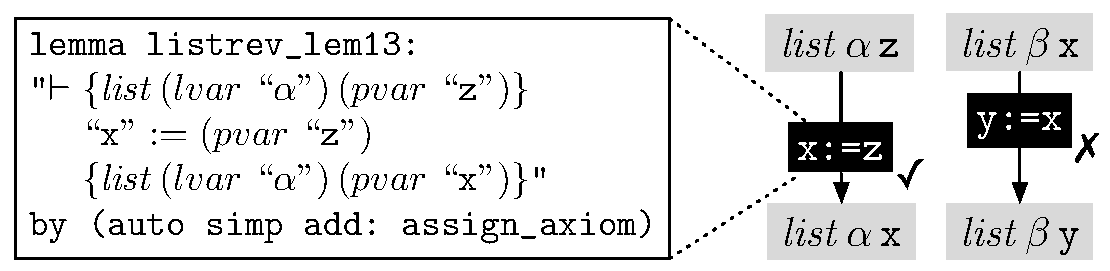
\includegraphics[width=85mm]{listrev_graph_mini.pdf}
\end{center}
In the current prototype, the user must supply the input in textual form, but in the future, we intend to enable direct interaction with the graphical representation, perhaps through a framework for diagrammatic reasoning such as \emph{Diabelli}~\cite{urbas+12}. We envisage an interactive graphical interface for exploring and modifying proofs, that allows steps to be collapsed or expanded to the desired granularity -- whether that is the fine details of every rule and axiom, or a coarse bird's-eye view of the overall structure of the proof.

The ribbon proofs in this paper have all been laid out manually (and we are preparing a public release of the {\LaTeX} macros we use to do this) but there is scope for additional tool support for discovering pleasing layouts automatically.

\section{Related and further work}\label{sect:future}

Ribbon proofs are more than just a pretty syntax; they are a sound and complete proof system. Proof outlines have previously been promoted from a notational device to a formal system by Schneider~\cite{schneider97}, and by Ashcroft, who remarks that ``the essential property of [proof outlines] is that each piece of program appears \emph{once}''~\cite{ashcroft76}. Very roughly speaking, ribbon proofs extend this property to each piece of assertion.

\begin{figure}[t]
\centering
\subfloat[ ]{
\label{fig:alternative_frame1}
\centering
\renewcommand{\arraystretch}{1}
\begin{tabular}{@{}l@{}}
\ass{\code{x}↦0 * \code{y}↦0 * \code{z}↦0} \\
~~\code{[x]:=1;} \\
\ass{\code{x}↦1 * \code{y}↦0 * \code{z}↦0} \\
\hspace{-1.2pt}~~$\left.\begin{tabular}{@{}l@{~~}l@{}}
\ass{\code{y}↦0 * \code{z}↦0} \\
~~\code{[y]:=1;} \\
\ass{\code{y}↦1 * \code{z}↦0} \\
~~\code{[z]:=1;} \\
\ass{\code{y}↦1 * \code{z}↦1}
\end{tabular}~~\right]\hspace{-5.5pt}\textrm{-}$ {\renewcommand{\arraystretch}{1}\begin{tabular}{@{}l@{}}frame\\ $\code{x}↦1$\end{tabular}} \\
\ass{\code{x}↦1 * \code{y}↦1 * \code{z}↦1}
\end{tabular}
}
\hspace{2cm}
\subfloat[ ]{
\label{fig:alternative_frame2}
\centering
\renewcommand{\arraystretch}{1}
\begin{tabular}{@{}l@{}}
\ass{\code{x}↦0 * \code{y}↦0 * \code{z}↦0} \\
\hspace{-1.2pt}~~$\left.\begin{tabular}{@{}l@{~~}l@{}}
\ass{\code{x}↦0 * \code{y}↦0} \\
~~\code{[x]:=1;} \\
\ass{\code{x}↦1 * \code{y}↦0} \\
~~\code{[y]:=1;} \\
\ass{\code{x}↦1 * \code{y}↦1}
\end{tabular}~~\right]\hspace{-5.5pt}\textrm{-}$ {\renewcommand{\arraystretch}{1}\begin{tabular}{@{}l@{}}frame\\$\code{z}↦0$\end{tabular}} \\
\ass{\code{x}↦1 * \code{y}↦1 * \code{z}↦0} \\
~~\code{[z]:=1;} \\
\ass{\code{x}↦1 * \code{y}↦1 * \code{z}↦1}
\end{tabular}
}
\caption{Two alternatives to the proof outline in Fig.~\ref{fig:proofoutline}}
\label{fig:alternative_frames}
\end{figure}

When constructing a proof outline, one can reduce the repetition by `framing off' state that is unused for several instructions. For instance, Fig.~\ref{fig:alternative_frame1} depicts one variation of Fig.~\ref{fig:proofoutline} obtained by framing off \code{x} during the latter two instructions; another option is to frame off \code{z} during the first two (Fig.~\ref{fig:alternative_frame2}). It is unsatisfactory that there are several different proof outlines for what is essentially the same proof. More pragmatically, deciding among these options can be difficult with large proof outlines. Happily, each of these options yields the same ribbon proof (Fig.~\ref{fig:assignment_ribbonproof}). We note a parallel here with \emph{proof nets}~\cite{girard87}, which are a graphical mechanism for unifying proofs in linear logic that differ only in uninteresting ways, such as the order of rule applications. 

The graphical structures in Defn.~\ref{defn:diagrams} resemble Milner's \emph{bigraphs}~\cite{milner09}. Assertions and commands are nodes, the deductions of the proof form the \emph{link graph}, and existential boxes, choices and loops form the \emph{place graph}. In fact, our diagrams correspond to \emph{binding} bigraphs, in which links may not cross place boundaries. Relaxing this restriction may enable a model of the `dynamic' scoping of existential boxes exhibited in Fig.~\ref{fig:dynamic_scoping}, which our current formalisation dismisses as a purely syntactic artefact.

Ribbon proofs can be understood as objects of a symmetric monoidal category, and our pictures as \emph{string diagrams}, which are widely used as graphical languages for such categories~\cite{selinger11}. In future work we intend to investigate this categorical semantics of ribbon proofs; in particular, the use of \emph{traces}~\cite{joyal+96} to model the loop construction depicted in Fig.~\ref{fig:ifwhilepic}a, and coproducts to model if-statements and existential boxes.

Another avenue for future work is the connection between ribbon proofs and Raza et al.'s \emph{labelled separation logic}~\cite{raza+09}. Labelled separation logic seeks to justify compiler reorderings by analysing the dependencies between program statements, and checking that these are not violated. The dependencies are detected by first labelling each component of each assertion with the commands that access it, and then propagating these labels through program proofs. Raza's labels recall the \emph{columns} in our ribbon diagrams: each ribbon and each command occupies one or more columns of a diagram, and commands that occupy common columns (modulo twisting) may share a dependency.

\begin{figure}[tp]
\centering
\begin{minipage}{40mm}
\subfloat[Code for `producer' thread]{
\begin{minipage}{40mm}
\begin{tabular}{l}
\code{while true \{} \\
\code{~x:=new();} \\
\code{~with buff when !full \{}\\
\code{~~full:=true; }\\
\code{~~ c:=x; }\\
\code{~\}} \\
\code{\}}
\end{tabular}
\end{minipage}
} \\[4mm]
\subfloat[Code for `consumer' thread]{
\begin{minipage}{40mm}
\begin{tabular}{l}
\code{while true \{} \\
\code{~with buff when full \{} \\
\code{~~full:=false;} \\
\code{~~y:=c;} \\
\code{~\}}\\
\code{~dispose(y);}\\
\code{\}}
\end{tabular}
\end{minipage}
}
\end{minipage}
~~~~~~~
\subfloat[Ribbon proof for `consumer' thread (mock-up)]{
\raisebox{2.5mm}{
\begin{minipage}{72mm}
\noindent%Starting.
\pgfdeclarelayer{frontmost}
\pgfdeclarelayer{colnameslayer}
\pgfsetlayers{main,frontmost,colnameslayer}
\begin{tikzpicture}[x=1mm,y=1mm,scale=0.9]
% State has been set.
\draw [line width = 0.6mm, \commandcolor] (1.65,-6.) -- (1.65,-5.);
\draw [line width = 0.6mm, \commandcolor] (25.35,-6.) -- (25.35,-5.);
\fill[fill=\commandcolor, rounded corners=1.8mm] (1.3,-5.) rectangle (25.7,0.);
\fill[fill=\commandcolor] (1.3,-5.) rectangle (25.7,-2.5);
\draw [white] (1.3,-2.5) node[anchor=west]{\code{while true \{}};
\draw [line width = 0.5mm, white] (28.,0.) -- (28.,-5.);
\draw [line width = 0.5mm, white] (79.,0.) -- (79.,-5.);
\fill [black!15] (28.,0.) -- (28.,-5.) -- (79.,-5.) -- (79.,0.) -- cycle;
\begin{pgfonlayer}{frontmost}
\draw [black] (53.5,-5.) node{\smash{$\ml[t]{(\code{full} ∧ \code{c}↦\underscore) ∨ (¬\code{full} ∧ \emp)}$}};
\end{pgfonlayer}
\draw [line width = 0.5mm, white] (28.,-5.) -- (28.,-7.);
\draw [line width = 0.5mm, white] (79.,-5.) -- (79.,-7.);
\fill [black!15] (28.,-5.) -- (28.,-7.) -- (79.,-7.) -- (79.,-5.) -- cycle;
\draw [line width = 0.6mm, \commandcolor] (1.65,-7.) -- (1.65,-5.);
\draw [line width = 0.6mm, \commandcolor] (25.35,-7.) -- (25.35,-5.);
\draw [line width = 0.6mm, \commandcolor] (3.65,-13.) -- (3.65,-12.);
\draw [line width = 0.6mm, \commandcolor] (80.35,-13.) -- (80.35,-12.);
% added {
\fill[fill=black!15, pattern color=white, pattern=north west lines] (28,0) rectangle (79,-7);
% }
\fill[fill=\commandcolor, rounded corners=1.8mm] (3.3,-12.) rectangle (80.7,-7.);
\fill[fill=\commandcolor] (3.3,-12.) rectangle (80.7,-9.5);
\draw [white] (3.3,-9.5) node[anchor=west]{\code{with buff when full \{}};
\draw [line width = 0.6mm, \commandcolor] (1.65,-12.) -- (1.65,-7.);
%\draw [line width = 0.6mm, \commandcolor] (25.35,-12.) -- (25.35,-7.);
\draw [line width = 0.6mm, \commandcolor] (3.65,-18.) -- (3.65,-12.);
\draw [line width = 0.6mm, \commandcolor] (80.35,-18.) -- (80.35,-12.);
\draw [line width = 0.6mm, \commandcolor] (1.65,-18.) -- (1.65,-12.);
%\draw [line width = 0.6mm, \commandcolor] (25.35,-18.) -- (25.35,-12.);
\draw [line width = 0.5mm, white] (5.,-12.) -- (5.,-18.);
\draw [line width = 0.5mm, white] (24.,-12.) -- (24.,-18.);
\fill [black!15] (5.,-12.) -- (5.,-18.) -- (24.,-18.) -- (24.,-12.) -- cycle;
\begin{pgfonlayer}{frontmost}
\draw [black] (14.5,-16.) node{\smash{$\ml[t]{\code{full}}$}};
\end{pgfonlayer}
\draw [line width = 0.5mm, white] (28.,-12.) -- (28.,-18.);
\draw [line width = 0.5mm, white] (79.,-12.) -- (79.,-18.);
\fill [black!15] (28.,-12.) -- (28.,-18.) -- (79.,-18.) -- (79.,-12.) -- cycle;
\draw [line width = 0.6mm, \commandcolor] (3.65,-19.) -- (3.65,-18.);
\draw [line width = 0.6mm, \commandcolor] (80.35,-19.) -- (80.35,-18.);
\draw [line width = 0.6mm, \commandcolor] (1.65,-19.) -- (1.65,-18.);
%\draw [line width = 0.6mm, \commandcolor] (25.35,-19.) -- (25.35,-18.);
\draw [line width = 0.6mm, \commandcolor] (3.65,-25.) -- (3.65,-19.);
\draw [line width = 0.6mm, \commandcolor] (80.35,-25.) -- (80.35,-19.);
\draw [line width = 0.6mm, \commandcolor] (1.65,-25.) -- (1.65,-19.);
%\draw [line width = 0.6mm, \commandcolor] (25.35,-25.) -- (25.35,-19.);
\draw [line width = 0.5mm, white] (5.,-19.) -- (5.,-25.);
\draw [line width = 0.5mm, white] (79.,-19.) -- (79.,-25.);
\fill [black!15] (5.,-19.) -- (5.,-25.) -- (79.,-25.) -- (79.,-19.) -- cycle;
\begin{pgfonlayer}{frontmost}
\draw [black] (42.,-23.) node{\smash{$\ml[t]{\code{full} ∧ \code{c}↦\underscore}$}};
\end{pgfonlayer}
\draw [line width = 0.6mm, \commandcolor] (3.65,-26.) -- (3.65,-25.);
\draw [line width = 0.6mm, \commandcolor] (80.35,-26.) -- (80.35,-25.);
\draw [line width = 0.6mm, \commandcolor] (1.65,-26.) -- (1.65,-25.);
%\draw [line width = 0.6mm, \commandcolor] (25.35,-26.) -- (25.35,-25.);
\draw [line width = 0.6mm, \commandcolor] (3.65,-32.) -- (3.65,-26.);
\draw [line width = 0.6mm, \commandcolor] (80.35,-32.) -- (80.35,-26.);
\draw [line width = 0.6mm, \commandcolor] (1.65,-32.) -- (1.65,-26.);
%\draw [line width = 0.6mm, \commandcolor] (25.35,-32.) -- (25.35,-26.);
\draw [line width = 0.5mm, white] (5.,-26.) -- (5.,-32.);
\draw [line width = 0.5mm, white] (24.,-26.) -- (24.,-32.);
\fill [black!15] (5.,-26.) -- (5.,-32.) -- (24.,-32.) -- (24.,-26.) -- cycle;
\begin{pgfonlayer}{frontmost}
\draw [black] (14.5,-30.) node{\smash{$\ml[t]{\code{c}↦\underscore}$}};
\end{pgfonlayer}
\draw [line width = 0.5mm, white] (28.,-26.) -- (28.,-32.);
\draw [line width = 0.5mm, white] (79.,-26.) -- (79.,-32.);
\fill [black!15] (28.,-26.) -- (28.,-32.) -- (79.,-32.) -- (79.,-26.) -- cycle;
\begin{pgfonlayer}{frontmost}
\draw [black] (53.5,-30.) node{\smash{$\ml[t]{\code{full} ∧ \emp}$}};
\end{pgfonlayer}
\begin{pgfonlayer}{frontmost}
\fill[fill=\commandcolor] (28.,-37.) rectangle (79.,-32.);
\draw [white] (28.,-34.5) node[anchor=west]{\code{\begin{tabular}{@{\hspace{-0.8mm}}l@{\hspace{-0.8mm}}}full := false\end{tabular}}};
\end{pgfonlayer}
\draw [line width = 0.5mm, white] (5.,-32.) -- (5.,-37.);
\draw [line width = 0.5mm, white] (24.,-32.) -- (24.,-37.);
\fill [black!15] (5.,-32.) -- (5.,-37.) -- (24.,-37.) -- (24.,-32.) -- cycle;
\draw [line width = 0.6mm, \commandcolor] (3.65,-37.) -- (3.65,-32.);
\draw [line width = 0.6mm, \commandcolor] (80.35,-37.) -- (80.35,-32.);
\draw [line width = 0.6mm, \commandcolor] (1.65,-37.) -- (1.65,-32.);
%\draw [line width = 0.6mm, \commandcolor] (25.35,-37.) -- (25.35,-32.);
\draw [line width = 0.6mm, \commandcolor] (3.65,-38.) -- (3.65,-37.);
\draw [line width = 0.6mm, \commandcolor] (80.35,-38.) -- (80.35,-37.);
\draw [line width = 0.6mm, \commandcolor] (1.65,-38.) -- (1.65,-37.);
%\draw [line width = 0.6mm, \commandcolor] (25.35,-38.) -- (25.35,-37.);
\draw [line width = 0.5mm, white] (5.,-37.) -- (5.,-38.);
\draw [line width = 0.5mm, white] (24.,-37.) -- (24.,-38.);
\fill [black!15] (5.,-37.) -- (5.,-38.) -- (24.,-38.) -- (24.,-37.) -- cycle;
\draw [line width = 0.5mm, white] (28.,-37.) -- (28.,-38.);
\draw [line width = 0.5mm, white] (79.,-37.) -- (79.,-38.);
\fill [black!15] (28.,-37.) -- (28.,-38.) -- (79.,-38.) -- (79.,-37.) -- cycle;
\begin{pgfonlayer}{frontmost}
\draw [black] (53.5,-41.) node{\smash{$\ml[t]{¬\code{full} ∧ \emp}$}};
\end{pgfonlayer}
\begin{pgfonlayer}{frontmost}
\fill[fill=\commandcolor] (5.,-43.) rectangle (24.,-38.);
\draw [white] (5.,-40.5) node[anchor=west]{\code{\begin{tabular}{@{\hspace{-0.8mm}}l@{\hspace{-0.8mm}}}y := c\end{tabular}}};
\end{pgfonlayer}
\draw [line width = 0.6mm, \commandcolor] (3.65,-43.) -- (3.65,-38.);
\draw [line width = 0.6mm, \commandcolor] (80.35,-43.) -- (80.35,-38.);
\draw [line width = 0.6mm, \commandcolor] (1.65,-43.) -- (1.65,-38.);
%\draw [line width = 0.6mm, \commandcolor] (25.35,-43.) -- (25.35,-38.);
\draw [line width = 0.5mm, white] (28.,-38.) -- (28.,-43.);
\draw [line width = 0.5mm, white] (79.,-38.) -- (79.,-43.);
\fill [black!15] (28.,-38.) -- (28.,-43.) -- (79.,-43.) -- (79.,-38.) -- cycle;
\draw [line width = 0.6mm, \commandcolor] (3.65,-44.) -- (3.65,-43.);
\draw [line width = 0.6mm, \commandcolor] (80.35,-44.) -- (80.35,-43.);
\draw [line width = 0.6mm, \commandcolor] (1.65,-44.) -- (1.65,-43.);
%\draw [line width = 0.6mm, \commandcolor] (25.35,-44.) -- (25.35,-43.);
\draw [line width = 0.5mm, white] (5.,-43.) -- (5.,-44.);
\draw [line width = 0.5mm, white] (24.,-43.) -- (24.,-44.);
\fill [black!15] (5.,-43.) -- (5.,-44.) -- (24.,-44.) -- (24.,-43.) -- cycle;
\begin{pgfonlayer}{frontmost}
\draw [black] (14.5,-47.) node{\smash{$\ml[t]{\code{y}↦\underscore}$}};
\end{pgfonlayer}
\draw [line width = 0.5mm, white] (5.,-44.) -- (5.,-50.);
\draw [line width = 0.5mm, white] (24.,-44.) -- (24.,-50.);
\fill [black!15] (5.,-44.) -- (5.,-50.) -- (24.,-50.) -- (24.,-44.) -- cycle;
\draw [line width = 0.6mm, \commandcolor] (3.65,-50.) -- (3.65,-44.);
\draw [line width = 0.6mm, \commandcolor] (80.35,-50.) -- (80.35,-44.);
\draw [line width = 0.6mm, \commandcolor] (1.65,-50.) -- (1.65,-44.);
%\draw [line width = 0.6mm, \commandcolor] (25.35,-50.) -- (25.35,-44.);
\draw [line width = 0.5mm, white] (28.,-44.) -- (28.,-50.);
\draw [line width = 0.5mm, white] (79.,-44.) -- (79.,-50.);
\fill [black!15] (28.,-44.) -- (28.,-50.) -- (79.,-50.) -- (79.,-44.) -- cycle;
\begin{pgfonlayer}{frontmost}
\draw [black] (53.5,-48.) node{\smash{$\ml[t]{(\code{full} ∧ \code{c}↦\underscore) ∨ (¬\code{full} ∧ \emp)}$}};
\end{pgfonlayer}
\draw [line width = 0.6mm, \commandcolor] (3.65,-50.) -- (3.65,-49.);
\draw [line width = 0.6mm, \commandcolor] (80.35,-50.) -- (80.35,-49.);
\fill[fill=\commandcolor, rounded corners=1.8mm] (3.3,-55.) rectangle (80.7,-50.);
\fill[fill=\commandcolor] (3.3,-52.5) rectangle (80.7,-50.);
\draw [white] (3.3,-52.5) node[anchor=west]{\code{\}}};
\draw [line width = 0.6mm, \commandcolor] (1.65,-55.) -- (1.65,-50.);
%\draw [line width = 0.6mm, \commandcolor] (25.35,-55.) -- (25.35,-50.);
\draw [line width = 0.5mm, white] (28.,-55.) -- (28.,-58.);
\draw [line width = 0.5mm, white] (79.,-55.) -- (79.,-58.);
\fill [black!15] (28.,-55.) -- (28.,-58.) -- (79.,-58.) -- (79.,-55.) -- cycle;
\draw [line width = 0.6mm, \commandcolor] (1.65,-58.) -- (1.65,-55.);
\draw [line width = 0.6mm, \commandcolor] (25.35,-58.) -- (25.35,-55.);
\draw [line width = 0.5mm, white] (5.,-55.) -- (5.,-58.);
\draw [line width = 0.5mm, white] (24.,-55.) -- (24.,-58.);
\fill [black!15] (5.,-55.) -- (5.,-58.) -- (24.,-58.) -- (24.,-55.) -- cycle;
\begin{pgfonlayer}{frontmost}
\fill[fill=\commandcolor] (5.,-63.) rectangle (24.,-58.);
\draw [white] (5.,-60.5) node[anchor=west]{\code{\begin{tabular}{@{\hspace{-0.8mm}}l@{\hspace{-0.8mm}}}dispose(y)\end{tabular}}};
\end{pgfonlayer}
\draw [line width = 0.5mm, white] (28.,-58.) -- (28.,-63.);
\draw [line width = 0.5mm, white] (79.,-58.) -- (79.,-63.);
\fill [black!15] (28.,-58.) -- (28.,-63.) -- (79.,-63.) -- (79.,-58.) -- cycle;
\draw [line width = 0.6mm, \commandcolor] (1.65,-63.) -- (1.65,-58.);
\draw [line width = 0.6mm, \commandcolor] (25.35,-63.) -- (25.35,-58.);
\draw [line width = 0.5mm, white] (28.,-63.) -- (28.,-65.);
\draw [line width = 0.5mm, white] (79.,-63.) -- (79.,-65.);
\fill [black!15] (28.,-63.) -- (28.,-65.) -- (79.,-65.) -- (79.,-63.) -- cycle;
\draw [line width = 0.6mm, \commandcolor] (1.65,-65.) -- (1.65,-63.);
\draw [line width = 0.6mm, \commandcolor] (25.35,-65.) -- (25.35,-63.);
\draw [line width = 0.6mm, \commandcolor] (1.65,-65.) -- (1.65,-64.);
\draw [line width = 0.6mm, \commandcolor] (25.35,-65.) -- (25.35,-64.);
\fill[fill=\commandcolor, rounded corners=1.8mm] (1.3,-70.) rectangle (25.7,-65.);
\fill[fill=\commandcolor] (1.3,-67.5) rectangle (25.7,-65.);
\draw [white] (1.3,-67.5) node[anchor=west]{\code{\}}};
\draw [line width = 0.5mm, white] (28.,-65.) -- (28.,-70.);
\draw [line width = 0.5mm, white] (79.,-65.) -- (79.,-70.);
\fill [black!15] (28.,-65.) -- (28.,-70.) -- (79.,-70.) -- (79.,-65.) -- cycle;
% added {
\fill[fill=black!15, pattern color=white, pattern=north west lines] (28,-55) rectangle (79,-70);
% }
\end{tikzpicture}
%Finished.
\vspace{-4mm}
\end{minipage}
\label{fig:buffer_proof}
}
}
\caption{Concurrency example: a single-cell buffer}
\label{fig:buffer}
\end{figure}

We have so far considered only sequential programs, but our proofs have a distinctly concurrent flavour. It may be possible to extend ribbon proofs to \emph{concurrent separation logic}~\cite{ohearn07} as follows.
Figure~\ref{fig:buffer} gives a program (adapted from~\cite{ohearn07}) in which two threads communicate through a shared buffer at location \code{c}. The \emph{resource invariant} \mbox{$(\code{full} ∧ \code{c}↦\underscore)$} $∨$ \mbox{($¬\code{full} ∧ \emp)$} protected by the lock \code{buff} signifies that \code{c} is shared exactly when \code{full} is set. Figure~\ref{fig:buffer_proof} imagines a ribbon proof of the `consumer' thread. The resource invariant is initially in a protected ribbon, inaccessible to the thread (as suggested by the hatching). Upon entering the critical region, the ribbon becomes available, and upon leaving it, the resource invariant is re-established and the ribbon is inaccessible once again.

Beyond concurrent separation logic, we intend to apply our system to more advanced separation logics. It has already aided the development of a logic for relaxed memory~\cite{bornat+12}; other candidates handle fine-grained concurrency~\cite{dinsdale-young+10-b,feng09,feng+07-a,vafeiadis+07}, dynamic threads~\cite{dodds+09}, storable locks~\cite{gotsman+07}, loadable modules~\cite{jacobs+11} and garbage collection~\cite{hur+11%,kapoor+11
}. Increasingly complicated logics for increasingly complicated programming features make techniques for intuitive construction and clear presentation ever more crucial.

\section{Conclusion}

Ribbon proofs are an attractive and practical approach for constructing and presenting proofs in separation logic or any derivative thereof. They contain less redundancy than a proof outline, and express the intent of the proof more clearly. Each step of the proof can be checked locally, by focusing only on the relevant resources. They are useful pedagogically for explaining how a simple proof is constructed, but also scale to more complex programs (as demonstrated in~\cite{wickerson13}), and have aided the development of a separation logic for relaxed memory~\cite{bornat+12}. They show graphically the distribution of resource in a program, and in particular, which parts of a program operate on disjoint resources, and this may prove useful for exploring parallelisation opportunities.

\paragraph{\bf Acknowledgements} Wickerson was supported by a DAAD postdoctoral scholarship and EPSRC grant F019394/1. Dodds was supported by EPSRC grants EP/H005633/1 and EP/F036345. Figure~\ref{fig:ifwhilepic} was drawn by Rasmus Petersen. We thank him, Nick Benton, Richard Bornat, Matko Botin\v{c}an, Daiva Naud\v{z}i\={u}nien\.{e}, Peter O'Hearn, Andy Pitts, Noam Rinetzky and the anonymous reviewers for suggestions and encouragement.


\bibliographystyle{abbrv}
\bibliography{esop}

\end{document}